\chapter{Introduction}
Getting children in touch with technology is important in todays technologically advanced society. In schools technology (specifically electrical engineering and programming) is often taught using robots. Robots are well suited for children since they allow interaction with the reality in contrast to arbitrary technology related exercises such as programming exercises which doesn't affect the real world.\cite[pp.16]{johnson2003children}\newline 
Since schools are required to save money, robots used for teaching stay property of the schools. Therefore children usually cannot take the robot home to work with it. In addition modification of robot is usually not permitted which reduces potential learning experiences. Giving students the full control over all possibilities of the robot requires them to own the robot. This requires to robot to be cheap, extensible and suitable for educational purposes.\newline
The development of a robot platform for educational purpose requires requirement engineering, market research and evaluation of robots which are already used in education. Once the research is completed a new robot platform can be constructed taking the research results into account. The goal is to develop such an educational robot platform with regard to the target user group, their needs and educational concepts.
\chapter{Requirement Analysis / Project Goals}
User group of a robot can be categorized into different groups regardless of their age:
\begin{description}
\item[Beginner] \hfill \\ Beginners have little to no experience with robots. They need extensive assistance to perform tasks such as soldering and programming. For programming graphical programming languages (such as minibloq\footnote{\url{http://blog.minibloq.org/}} or ModKit\footnote{\url{http://www.modkit.com/}}) or languages providing a high level of abstraction (such as Wiring), 
\item[Advanced] \hfill \\ Advanced users have advanced experience with robots and robotics. Most programming and soldering tasks are done independently; working knowledge is utilized to solve new and unknown tasks.  
\item[Expert] \hfill \\ Expert users understand all aspects of robots and their internals. New challenges are faced with ease.
\end{description}

The target user group for this educational robotic project are beginners of all age with focus of children at school with limited budget. Teaching the knowledge requires a platform which is designed to be educational. Therefore it has to comply with several requirements which affect technical aspects as well as social aspects.
The following lists describes the basic requirements on which existing platforms can be assessed. The assessment criteria can also be used to make decisions when developing a new platform.
\begin{description}
\item[Affordable] \hfill \\ The robot platform must be affordable for everyone. Especially when the robot is used in schools every child should own the robot to increase the possibilities to modify and extend it. Robots which stay property of a school may result in social problems since socially disadvantaged children cannot afford their own robot whereas socially advantaged children can. A considerable price tag for a educational robot is the educational budget for a welfare recipient which is 100 Euro per year in Germany as defined defined in SGB II §28 (as of the 07.05.2013).
\item[Educational] \hfill \\ Documentation, learning materials and suggestions for lessons are needed to teach the usage of the robot. The robot should be designed to teach both electrical engineering as well as programming. This can be realized by having exercises specific to the topic e.g. by soldering the robot first with programming afterwards. If the platform supports both, graphical programming languages for young children as well as high-level programming languages the platform is more accessible for education. 
\item[Sustainable] \hfill \\ Sustainability is an environmental issue which should be taken into account. Sustainability includes several aspects such as the choice of materials, their durability and the repairability. It is a huge bonus if materials are environment-friendly and produced in a socially acceptable manner (tantalum capacitors for instance should be avoided for those reasons). If the robot can be easily repaired or interchanged using household or easy to get items the robot can be considered sustainable. 
\item[Extendable] \hfill \\ Extendability enables the robot to adapt to new tasks. Interchangeable sensors and actuators are the key to a flexible platform. The platform should provide some unused microcontroller pins dedicated to extensions. Those pins should be mapped onto easy accessible pins which require no soldering.  
\item[Trouble-free] \hfill \\ Building the robot should be a smooth, trouble free, task. Error sources should be prevented e.g. by using connectors which fit in one direction only or properly marked electric parts. Bending or modifying shipped parts should be avoided since it  could render the part broken or malfunctioning. Replacement parts should be easy to order or included within the robot kit (parts such as small SMD resistors which are very cheap).
\item[Open-Source] \hfill \\ Open-Source products can be easily modified, extended and remixed into new, continuously improved, products. Schematics, PCB layout files, build-instructions and specifications should be accessible under a permissive open-source license. 
\end{description}

In the following chapters the state of the art in robotics is evaluated, robotic components are assessed and the construction of the robot according to the requirements is presented in detail and critically discussed. The structure is aimed to give a big picture and get into detail as more and more components are introduced.
\chapter{State of the Art}
The development of a new robot platform requires the assessment of current robotic platforms using the requirements developed. In focus of the assessment are popular robot platforms which are either actively used in schools or developed with education in mind. All of the platforms are independently developed and focus on different ideas. 

Assessment criteria are evaluated using a rating system which allows values between zero and five where higher values are better. Each value is represented using stars for better overview. Detailed description of each rating is explained below.

\begin{description}
\item[\stars{5}] \hfill \\The evaluated aspect fully complies with the assessment criteria and adds additional functionality which exceeds expectations. 
\item[\stars{4}] \hfill \\The evaluated aspect fully complies with the assessment criteria. Mentioned properties may have minor restraints which do not affect the overall quality/functionality of the system.
\item[\stars{3}] \hfill \\The evaluated aspect complies with most of the assessment criteria. The evaluation shows that some minor and/or major restraints exist which may affect the overall quality/functionality.
\item[\stars{2}] \hfill \\The evaluated aspect meets the assessment criteria partially but shows severe restraints affecting the overall quality/functionality.
\item[\stars{1}] \hfill \\The evaluated aspect contains the rudiments of the assessment criteria.
\item[\stars{0}] \hfill \\The evaluated aspect does not met the assessment criteria in any way. 
\end{description}

\section{Asuro}
\begin{figure}[h!]
  \centering
  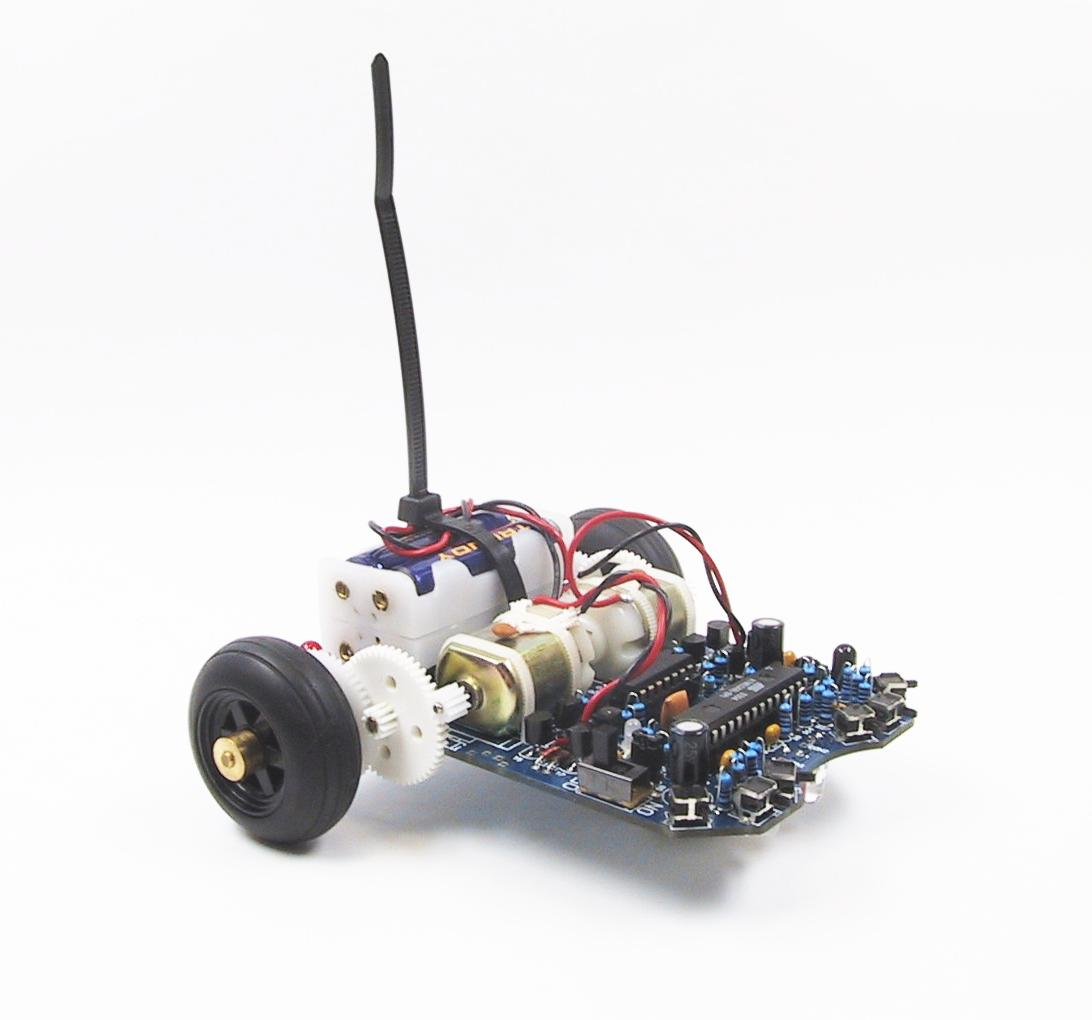
\includegraphics[width=0.5\textwidth]{images/asuro.jpg}
  \caption{Picture of the Asuro (CC-BY-SA Robin Gruber)}
\end{figure}

The Asuro robot is developed by the German Aerospace Center (Deutsches Zentrum für Luft- und Raumfahrt e.V.) in cooperation with Arexx Engineering focused on educational use. Classroom courses, educational material and workshops were given using Asuro. Asuros development started in 2004 and is now discontinued. The robot is shipped as a do-it-yourself kit and requires about eight hours build time for a novice. 

Asuro features an eight bit Atmel ATmega8L microcontroller with eight kilobytes of flash memory, 512 bytes of electrical erasable programmable read only memory (short EEPROM) and one kilobytes of static random-access memory (short SRAM). One kilobyte of flash is used for the bootloader which results in seven kilobytes of flash usable for user programs. User programs are uploaded using a infrared serial connection.

Interaction with the environment is realized using two DC motors which can be controlled individually in terms of direction and speed. The robot is stabilized using a half table-tennis ball mounted at the bottom of the robot. Four LEDs are used for displaying the status of the Asuro. The whole system is powered by four AAA batteries or rechargeable batteries mounted in a 2x2 battery case. 

Asuro can sense its environment using different sensors such as two photodiodes which can be used for line-following tasks, six push buttons to detect objects in front of Asuro and two photoelectric sensors to determine the rotation speed of each of Asuros wheels.


\begin{longtabu} to \textwidth { X[1,l] X[1,l] X[4,l]}
\toprule
Assessment Criteria    & Rating & Description \\
\midrule
Affordable      & \stars{5}    & Having a price tag of 50 Euro renders the Asuro very affordable in comparison to the 100 Euro limit set. The cost effectiveness is outstanding and features sensors and actuators for basic tasks.     \\
Educational     & \stars{3}     & Asuro features detailed build-instructions in English and German. The guide also includes a tutorial on how to program Asuro in C. Even though there are a lot of opportunities to teach electrical engineering, the available documents do not explain the electrical usage and functional principle of each part. \\
Sustainable       & \stars{4}     & Asuro uses standard components only and features ROHS compliant parts which are free from heavy metals such as lead (PB). A broken Asuro can be easily repaired using the tools which are required to solder it. \\
Extendable & \stars{2}      & Having no free microcontroller pins and no broken out pins, Asuro cannot be considered extendable. There exist some hardware modification in the Asuro community which extend the functionality but require to unsolder/remove some parts.  \\
Trouble-free & \stars{3} & Building Asuro is well documented but some steps may lead to frustration. Mounting the axis using solder is very difficult and may burn the PCB due to the heat emitted in this process. Another frustrating task is to program the robot using the infrared serial connection, since this method is prone to interference. \\
Open-Source & \stars{4} & Asuro was licensed under the DLR-license which is transitioned into a Creative-Commons license model. Everything except the PCB layout files are available for download on the Asuro website.\\
\bottomrule
\caption{Asuro evaluation}
\label{tbl:asuro_eval}
\end{longtabu}

All in all the Asuro is a cost effective robot platform suitable for beginners. The lack of extendability and some difficult steps during the build lower the overall good rating to an average of 3.5 stars. 

\section{Arduino Robot}
\begin{figure}[H]
  \centering
  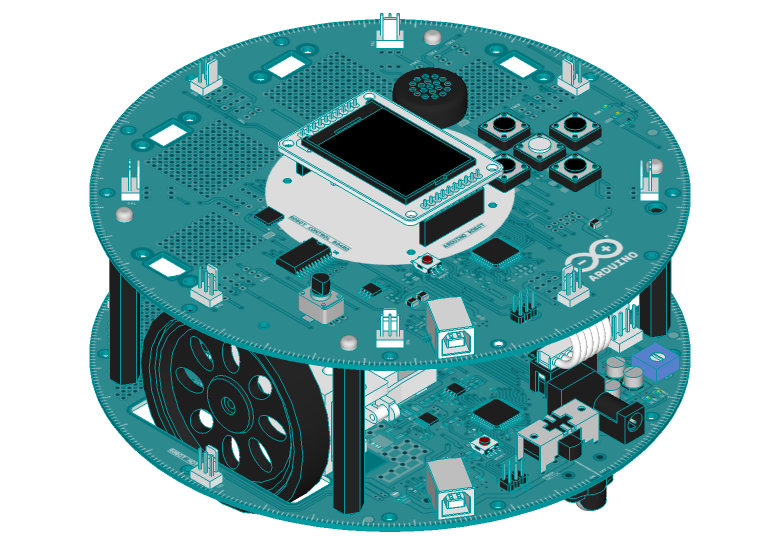
\includegraphics[width=0.5\textwidth]{images/arduinorobot.jpg}
  \caption{Rendering of the Arduino Robot (CC-BY-SA arduino.cc)}
\end{figure}

The Arduino Robot is the first robot created by the Arduino foundation targeted to educational purposes. It comes preassembled and consists of two different boards: the motor board and the control board. Due to this design, the Arduino robot contains two Atmel ATmega 32U4 microcontroller featuring a clock speed of 16MHz, 32KB of flash memory (of which 28KB can be used for user programs), 2.5KB of RAM and 1KB of EEPROM each.\footnote{{http://arduino.cc/en/Main/Robot}}

Each board can be individually programmed using the freely available Arduino IDE\footnote{\url{http://arduino.cc/en/Main/Software}} having the Robot connected to the computer using an USB cable. The IDE provides a lot of examples for the robot platform and introduces a library for abstract access to the robots functionaly. Power is applied to the system using four rechargeable NIMH-batteries which can be directly recharged on the board by connecting an appropriate power source to the board.

The robot can interact with its environment using movement generated by two controllable DC motors attached to wheels and stabilized using two ball caster. In addition to movement the robot can play sounds using a small speaker on the control board and display text and images on the display mounted on the control board as well. In contrast to the actuators the user can interact with the robot using buttons and several sensors such as infrared sensors for line following tasks or distance measurement.

\begin{longtabu} to \textwidth { X[1,l] X[1,l] X[4,l]}
\toprule
Assessment Criteria    & Rating & Description \\
\midrule
Affordable      & \stars{2}    & With a price tag of 189 Euro without VAT\footnote{As of 05.03.2014 from the official Arduino store: \url{http://store.arduino.cc/index.php?main_page=product_info&cPath=11_12&products_id=290}} the Arduino Robot is far above the price limit of 100 Euro. The price for the basic robot is very high compared to its features.\\
Educational     & \stars{3}     & The Arduino robot comes pre-built and therefore lacks the build experience. Learning material for teachers is not provided but a lot of examples and a library to ease programming is provided. Instructions for other Arduino products can be easily adapted to the robot. \\
Sustainable       & \stars{4}     &  The robot integrates charging circuit for the NIMH batteries eliminates the need of a dedicated battery charger and therefore reduces the amount of electrical waste. A small restraint is the choice of components because they cannot be interchanged/repaired by beginners. This is due to the manufacturing process which requires SMD components to be cost effective. Through hole parts would be easier to interchange but require manual assembly which is very expensive.\\
Extendable & \stars{5}      &  Having prototyping areas directly on the control board, the robot can be considered extendable. Moreover connectors for additional sensors are populated all over the robot board making it possible and easy to add sensors without soldering.\\
Trouble-free & \stars{4} & Since the Arduino robot comes pre-assembled and tested in factory, the robot can be called trouble-free. Transportation defects like loose screws can be repaired using household items. The usage is very simple and straight-forward.\\
Open-Source & \stars{3} & Even though it is claimed that the Arduino robot is open-source, not all files required for building the robot are published. The website is missing the PCB design files and includes the schematics only. A software library is available under a open-source license. \\
\bottomrule
\caption{Arduino Robot evaluation}
\label{tbl:arduinorobot_eval}
\end{longtabu}

To sum it up the Arduino robot is an extendable robot platform which requires no assembly at all. The integrated battery charging makes it a sustainable robot but the high price reduces the overall rating to an average of 3.5 stars.

\section{LEGO Mindstorms NXT 2.0}
\begin{figure}[H]
  \centering
  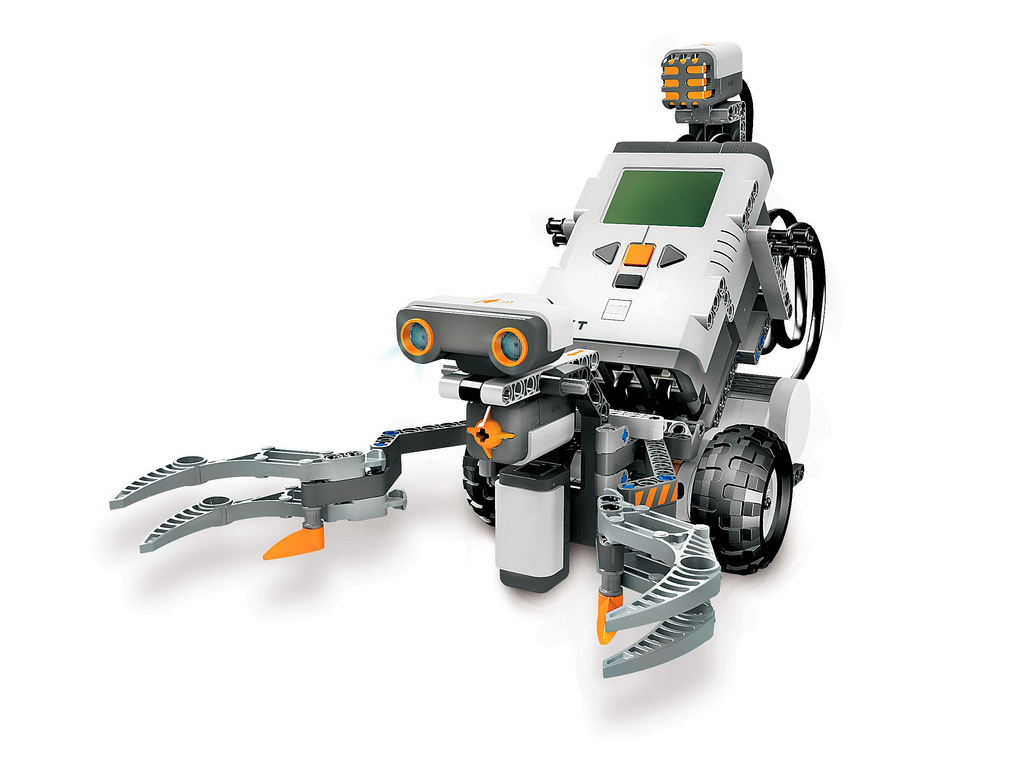
\includegraphics[width=0.5\textwidth]{images/mindstorms.jpg}
  \caption{Picture of the LEGO Mindstorms NXT (CC-BY-NC Elvis Ripley)}
\end{figure}

The LEGO Mindstorms NXT 2.0 platform was released by LEGO in 2009 and replaced the first LEGO Mindstorms NXT generation. It is compatible with Lego technic and therefore very flexible/extendable and aims at educational (Education Kit) and personal use (Inventor Kit). It is one of the most successful robotics system in education and is in wide use.

LEGO Mindstorms NXT is available in two different kits: the educational kit and a consumer kit. The NXT intelligent brick is the core of the robot platform and contains an 32-bit Atmel ARM7 core with 256KB of Flash memory, 64KB of RAM and supports bluetooth and usb communication to communicate with a host computer. Moreover the brick features a greyscale display, a speaker and four buttons for direct interaction with the brick.

The brick can be powered by using six AA batteries or a rechargeable Lithium-Ion battery with integrated charger which can be separately brought. Sensors and actuators are powered by the brick. A total of four sensors and three actuators can be attached to the brick using flexible cables with a position encoded modular connector.

In the standard kit three continuous rotation servo motors with one degree of accuracy are supplied as well as two touch sensors, one color sensor and an ultrasonic sensor. 

The consumer kit has a price tag of 279 Euro and the education basis set a price tag of 368.99 Euro + 89.24 Euro for the education software.

\begin{longtabu} to \textwidth { X[1,l] X[1,l] X[4,l]}
\toprule
Assessment Criteria    & Rating & Description \\
\midrule
Affordable  & \stars{2}    & With a price tag of 279 Euro (retail consumer edition) and 368.99 Euro (education version) the robot is far beyond the price tag of 100 Euro. The amount of sensors and actuators is low compared to the price.\\
Educational & \stars{5}     & LEGO provides a lot of resources for teaching and personal education using the Mindstorms NXT 2.0. Even though the electrical components are not subject, the set can teach a lot of knowledge and even interdisciplinary content. The flexibility of the robot allows the transformation of the robert for a lot of education concern. \\
Sustainable  & \stars{3}     & The Mindstorms NXT 2.0 set cannot be repaired using household items. Nevertheless the components are considered sustainable to a certain extend, since they are designed to be robust and to last a long time.\\
Extendable & \stars{3} & The robot can be extended up to a certain extend. Even though the specification for each interface is public available custom sensors are rare and/or expensive. \\
Trouble-free & \stars{5} & Using the platform is trouble free and easy. The LEGO Mindstorms IDE is intuitional. Support for different programming languages such as Java exist. A huge community and a lot of resources are available.\\
Open-Source & \stars{4} & LEGO open sourced the LEGO Mindstorms NXT brick and moreover the specification for each connector and sensor. The PCB design files and the casing are not open-sourced to prevent unauthorized replicas.\\
\bottomrule
\caption{Lego Mindstorms evaluation}
\label{tbl:mindstorms_eval}
\end{longtabu}

All in all the LEGO Mindstorms NXT 2.0 is a great robot platform with a lot of possible applications due to its compability with other LEGO products. The only drawback is the price which is not affordable for everyone.

\section{Thymio II}
\begin{figure}[H]
  \centering
  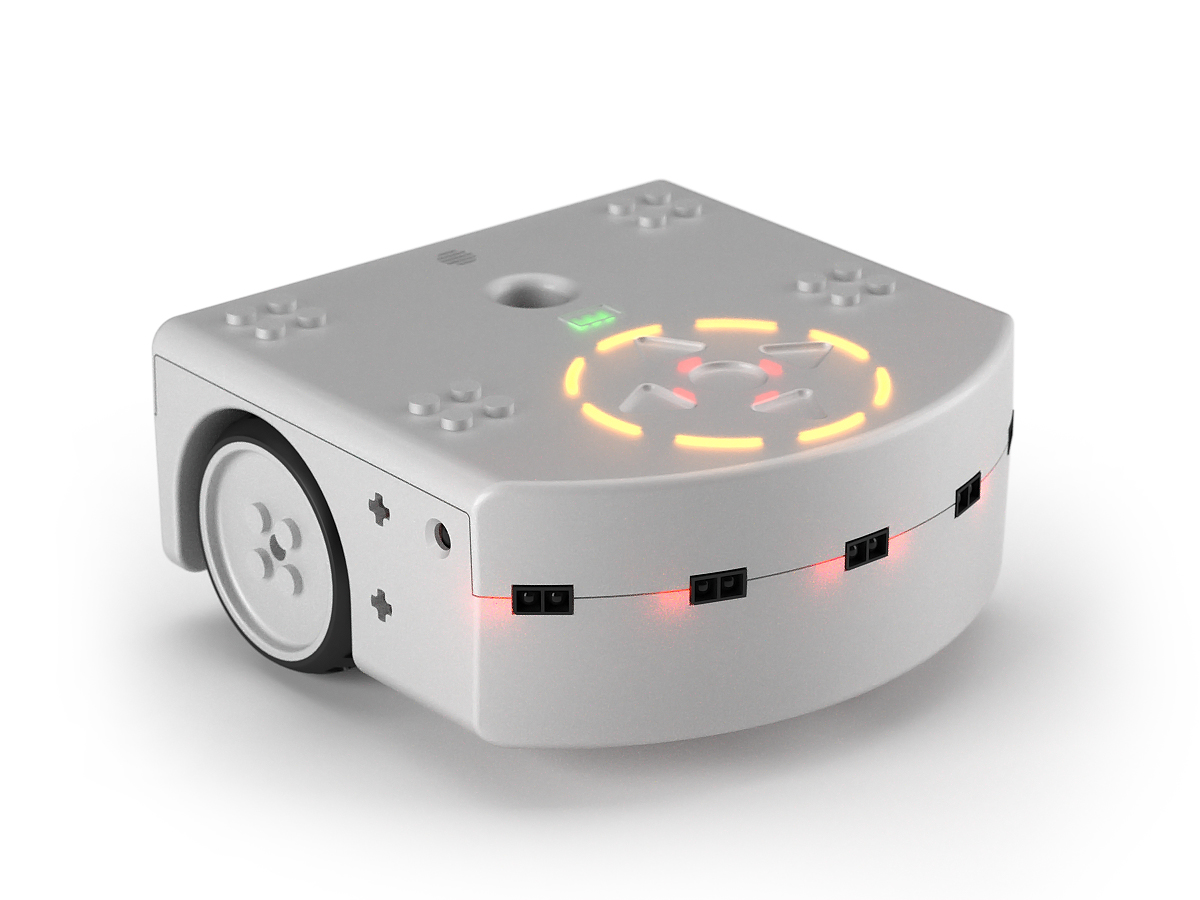
\includegraphics[width=0.5\textwidth]{images/thymioii.jpg}
  \caption{Picture of the Thymio II (CC-BY-SA Thymio II project team)}
\end{figure}

Thymio II is a robot developed by the Ecole Polytechnique Fédérale de Lausanne and the Ecole Cantonale d'Art de Lausanne for educational purposes. The robot comes preassembled and has a price tag of 99 CHF (plus taxes). It features a 16-bit PIC Microcontroller from Microchip with 128KB Flash, 16KB RAM and a clock Frequency of 8MHz. Programming is archieved using the integrated USB connection

The robot can show its state using several LEDs which illuminate parts of the robots body. It interacts with its environment using two motors and of course the LEDs included. Sensing the environment is archieved using several infrared distance sensors, a microphone, capacitive touch sensors, an accelerometer and a temperature sensor. Data can be stored on a external memory card.

Additional components can be mounted using LEGO compatible mechanical fixation points and an additional Thymio can be attached using the trailer hook. Various support for programming languages exist which adress beginners as well as advanced users.


\begin{longtabu} to \textwidth { X[1,l] X[1,l] X[4,l]}
\toprule
Assessment Criteria    & Rating & Description \\
\midrule
Affordable  & \stars{4}    & 99 CHF (without taxes directly from the Ecole Polytechnique Fédérale de Lausanne) is a reasonable price for a robot with this huge amount of features. On retail stores the price is higher due to profit margin.\\
Educational & \stars{3}     & Thymio II does not yet have a repository of educational material only, but it is planned to release such material. The compability with LEGO is a huge bonus, and creates a lot of pplications on which educational problems can be explained and demonstrated.\\
Sustainable  & \stars{3}     & The robot consists of small SMD parts and therefore parts cannot be replaced by the target user group. Materials used are suitable for children and designed to last. The integrated Li-Po battery can be recharged and therefore produces less environmental waste.\\
Extendable & \stars{3} & Except the LEGO compatible fixation points, Thymio II is not extendable without unsoldering components. On the software side, the choice of microcontroller supports a lot of additional program features.\\
Trouble-free & \stars{4} & Thymio II is trouble free since it comes preassembled and the usage is straight forward.\\
Open-Source & \stars{5} & Everything needed to build the robot is licensed under a permissive creative commons license. Program files and libraries are licensed under a LGPL license. Even the CAD files for the plastic mold injection parts are available without a charge.\\
\bottomrule
\caption{Thymio II evaluation}
\label{tbl:thymio_eval}
\end{longtabu}

To sum it up the Thymio II platform comes at a great price equipped with a lot of sensors. Its LEGO compatible fixation points are a huge bonus, the license of each aspect of the robot is very permissive. The overall rating of 3.66 stars reflects the huge potential of the platform. Once the educational material is available the platform is considerable as a educational platform.

\chapter{Case studies}
A robot is built using parts and modules which can be grouped into functional groups like movement, sensors or communication. The goal of each functional group can be achieved in various ways which have to be evaluated using the requirements used in the evaluation of other robot platforms. Some evaluation critera such as the fulfillment of the educational aspect or the open-source aspect may not be suitable for evaluation of single components and therefore left out. The Extendability describes the amount of microcontroller pins where the lesser amount of pins is considered better since this leaves space for extensions. Other difficulties in the evaluation process are dependencies between different modules, e.g. when a sensor has special power requirements. Based on the evaluation the robot will be constructed.
\section{Movement}
Movement is the most important feature since it allows the robot to interact with its environment. In contrast to a stationary robot, a moving robot can interact with a wider area but requires battery power or similar mobile energy sources. Different approaches for robot movement exist which will be part of critical evaluation.

There exist wheeled, legged, flying, swimming, diving and much more robot movement types. Wheeled robots are common since their mechanic principle is rather simple, cheap and easy to implement and control. Therefore other mentioned movement techniques except wheeled robots are not part of the evaluation.

\begin{figure}[H]
  \centering
  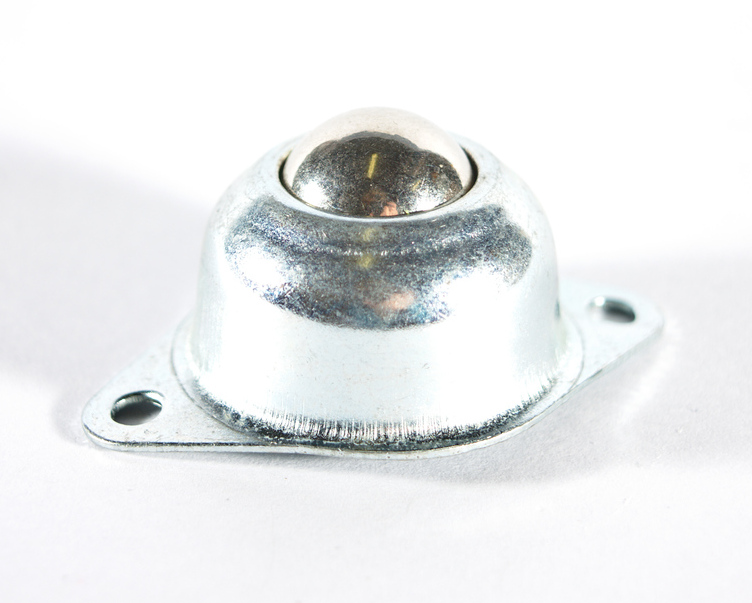
\includegraphics[width=0.5\textwidth]{images/30_ballcaster.jpg}
  \caption{Metal ball caster (CC-BY-SA Ben Oswald)}
\end{figure}


Typically robots have two wheels and a ball caster which prevents the robot from falling over. A ball caster acts as a third unidirected wheel with reduced friction. Alternatively four wheels and a steering mechanism or three wheels using omniwheels can be used. All types of wheeled robots can move in flat terrain and tolerate slight uneven surfaces. The outdoor usage is limited.
\subsection{Wheeled with two DC motors}
DC motors (direct current motors) are a cheap solutions for driving wheels. Usually a gear box is required to reduce the motor speed in favor of torque. Controlling the direction (forward and backward) requires the ability to switch the direction of the current flow. This is usally archieved using a H-bridge which can be found in as an integrated circuit or build using four electrical switches. 

There exist integrated circuits which provides two H-bridges combined in one component which allow the control of steering beneath the control of direction. Speed control is controlled by an external PWM (pulse-width-modulation) source.

\begin{figure}[H]
  \centering
  \begin{subfigure}{0.48\textwidth}
  \centering
  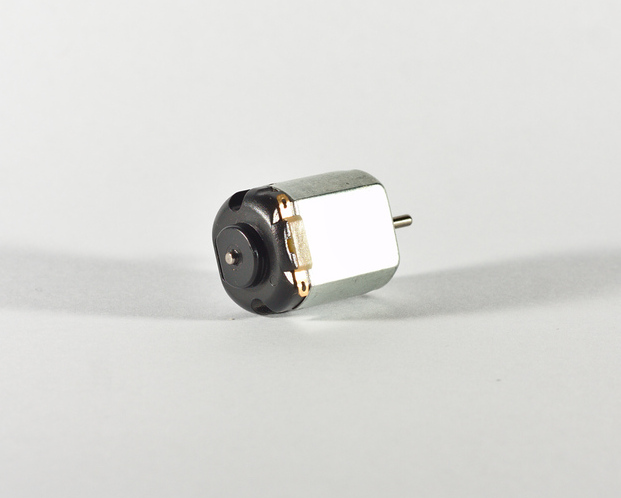
\includegraphics[width=0.9\linewidth]{images/30_dcmotor.jpg}
  \caption{Standard DC motor}
  \end{subfigure}
  \begin{subfigure}{0.48\textwidth}
  \centering
  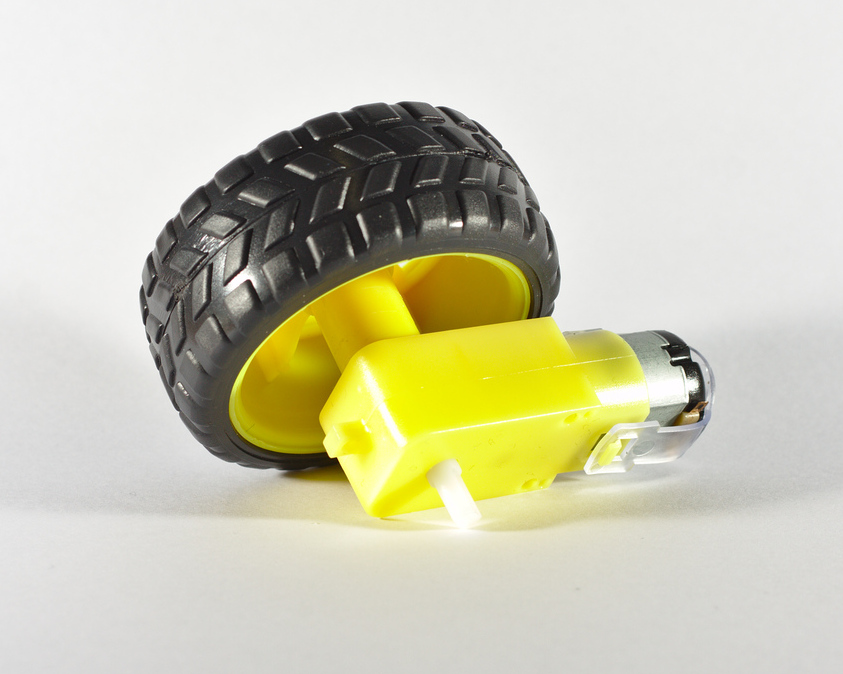
\includegraphics[width=0.9\linewidth]{images/30_gearboxmotor.jpg}
  \caption{Gearbox motor with wheel}
  \end{subfigure}
  \caption{Different DC motor types (CC-BY-SA Ben Oswald)}
\end{figure}

In terms of cost effectiveness a solution with two wheels powered by a DC motor each performs well. A DC motor with integrated gearbox is available for 5.5 USD, the plastic wheel costs 3.5 USD, a motor driver such as the L293 costs about 3.5 USD rendering a total cost of 21.5 USD per robot. In addition speed sensors for each of the wheels are needed since the motors do not have exactly the same speed since they are subject to variation during the production process. Without speed control sensors the robot may not drive straight forward. A simple sensor based on a rotating encoder disk and a light beam which is interrupted by the disk is available from 0.3 USD and requires one microcontroller pin per wheel (a microcontoller pin with interrupt support is the most reliable solution).

\begin{figure}[H]
  \centering
  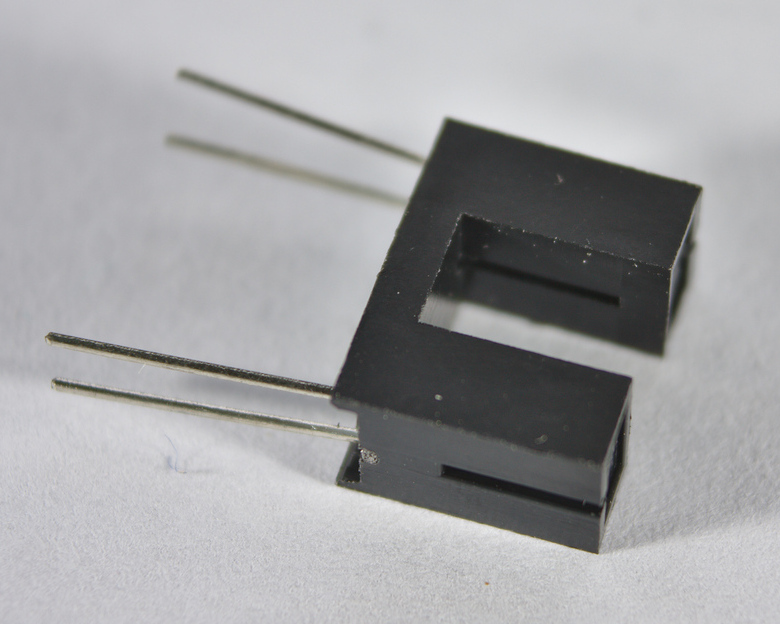
\includegraphics[width=0.5\textwidth]{images/30_speedsensor.jpg}
  \caption{Speedsensor (CC-BY-SA Ben Oswald)}
\end{figure}

The mentioned gearbox cannot be repaired once broken and should be replaced rather than repaired. Moreover it is unclear which materials are used in the plastic parts and whether they can be recycled. Mounting and controlling the motors is trouble free and requires at least six microcontroller pins as one can see in the following table.

\begin{table}[H]
\centering
\begin{tabular}{p{0.15\textwidth}p{0.15\textwidth}p{0.5\textwidth}}
\toprule
Pin count & Pin type & Description \\
\midrule
2 & PWM  & Motor speed control using pulse-width-modulation.\\
4 & GPIO & Direction control and steering control using a 4-bit (16 combinations) pattern.\\
\bottomrule
\end{tabular}
\caption{DC motor microcontroller pin usage}
\label{tbl:dc_pin}
\end{table}

When using a shift register for setting the four GPIO inputs of the motor driver, the pin count on the microcontroller can be reduced to three pins (Clock, Serial Data, Enable).  A single shift register can provide eight GPIO port and can be chained. 


\subsection{Wheeled with two Stepper motors}
Stepper motors are basically DC motors with more coils. In stepper motors the full rotation is divided into a number of equal steps which can be separately controlled. The motor can step forward, backward or hold the current position with huge torque. Stepper motors are usually shipped within a gear box which reduces steps much further to gain higher precision and torque. 
In typical applications stepper motors are driven by a dual H-bridge or darlington arrays attached to shift registers. The latter method is very cost effective but limited in current supply, the first method utilized a motor driver such as the L293 per stepper.

Stepper motors are availble for about 5 USD (in the USA\footnote{http://www.adafruit.com/products/858}). Two stepper motors are needed to drive the robot, an additional ball caster is needed to stabilize the movement. As mentioned in the forehand the cost of driving a stepper motor can be reduced using a shift register such as the 74HC595 in combination with a darlington array such as the ULN2803. Costs for this solution are about 12 USD where the stepper motors cost 10 USD, and the integrated circuits about 2 USD.

The pin usage on the microcontroller using the shift register is as follows:

\begin{table}[H]
\centering
\begin{tabular}{p{0.15\textwidth}p{0.15\textwidth}p{0.5\textwidth}}
\toprule
Pin count & Pin type & Description \\
\midrule
1 & GPIO & Clock which clocks the serial data. Not time critical due to the design of a shift register.\\
1 & GPIO & Serial data in which sets the bit pattern.\\
1 & GPIO & Chip enable which enables the shift register output.\\
\bottomrule
\end{tabular}
\caption{Shift register microcontroller pin usage}
\label{tbl:74hc595_pin}
\end{table}

Since shift registered are chainable, several stepper motors can be controlled using three pins only. A typical 74HC595 shift register has a settle time of 13 nanoseconds which allows 76900 switch cycles per second. For an eight bit shift register about 9600 full state changes can be performed, each additional shift register reduces the amount by half.

If a stepper motor gets broken, it can be easily replaced using the same model of stepper motor. Since the wheel is not part of the stepper motor, the old wheel can be replaced easily.
\subsection{Omniwheels}
Omniwheels/Mecanum wheels are the most flexible way of moving using wheels. Omniwheels are a special form of wheels which allow the movement in any direction having three independently moveable wheels. It requires three motors (typically DC motors) with direction control and optional speed control.

\begin{figure}[H]
  \centering
  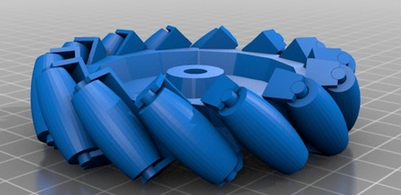
\includegraphics[width=0.5\textwidth]{images/mecanum.png}
  \caption{Screenshot of a mecanum wheel 3D model (from \url{http://www.thingiverse.com/thing:2318})}
\end{figure}

Integrating omni wheels into the robot plattform reduces the need of ball caster for stabilization but increases costs due to the need of an additional motor and motor controller. Moreover omni wheels itself have a price tag of 4 USD each which sums up to 12 USD for the wheels, three motors for 5.5 USD and two motor drivers for 3.5 USD each. This renders a cost of 35.5 USD plus the speed sensors which adds to even more. 

The pin usage is similar to the pin usage of wheeled robots with two DC motors. The control is more difficult since the control scheme is complex due to the movement vectors as shown in the figure \ref{fig:omnicontrol}.

\begin{figure}[H]
  \centering
  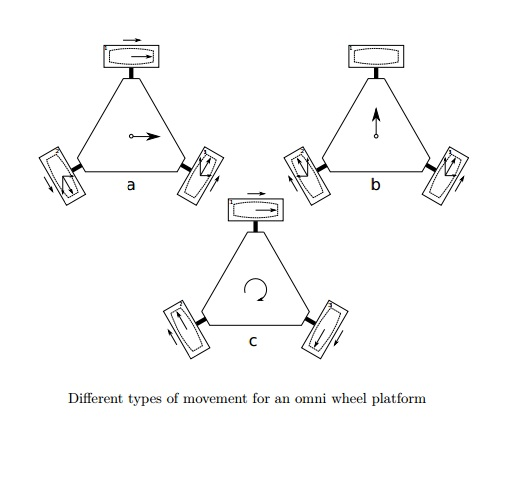
\includegraphics[width=0.5\textwidth]{images/omniwheel.jpg}
  \caption{Control scheme of a omni wheel (from \url{http://commons.wikimedia.org/wiki/File:Omni\_wheel\_control.jpg})}
  \label{fig:omnicontrol}
\end{figure}


\subsection{Conclusion}
All in all a solution using stepper motors with darlington array connected to shift registers is the most cost-effective solution. It provides the necessary functions and complies to the evaluation aspects such as the educational potential. Its usage is rather trouble free when apropriate libraries for motor control are provided.

\section{Sensors}
Sensors are important to make the robot sense its environment. Sensing the environment enables interaction such as obstacle avoidance, finding objects or following lines. Connecting sensors to a microcontroller can be done in various ways using various protocols. Different protocols require a different amount of microcontroller pins. Dependening on the sensor technology more or less computing time is needed to evaluate the sensors value.  

\subsection{IR Reciever}
Infrared Reciever are special photodiodes which react on infrared light with a base frequency of 38kHz. To ease the use of IR recievers with microcontrollers, the photodiode in the IR reciever has an integrated Schmitt trigger and therefore provides a near binary square voltage waveform instead of rising voltages. The cost of such a reciever is about 0.3USD.

\begin{figure}[H]
  \centering
  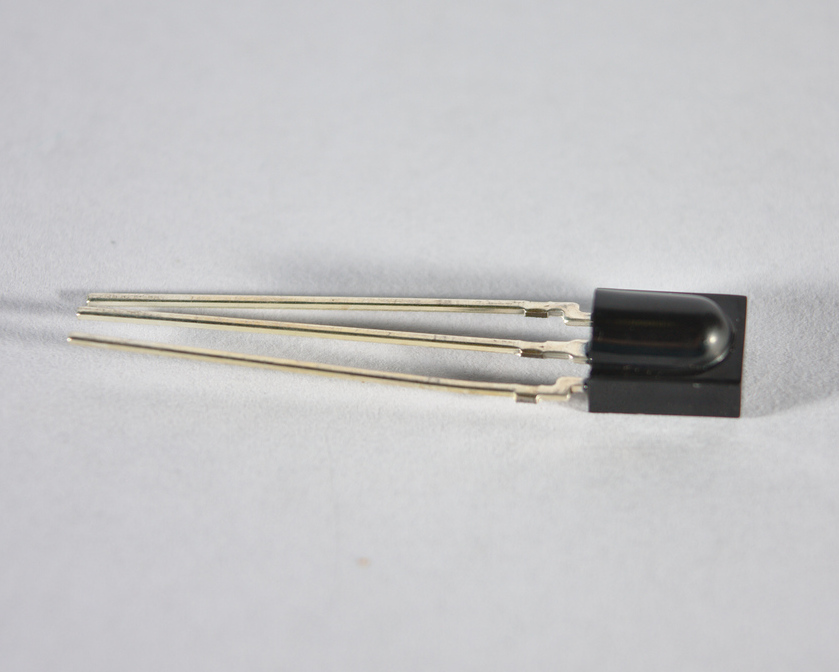
\includegraphics[width=0.5\textwidth]{images/30_ir.jpg}
  \caption{IR Reciever with integrated Schmitt trigger (CC-BY-SA Ben Oswald)}
\end{figure}

IR recievers are widely used in remote control applications such as televisions and remote controlled toys. Sending a signal requires a LED which emits light in the infrared spectrum. Cheap multipurpose remotes (about 1 USD) can be used to control own applications. Infrared beacons which steadily send a signal can be used to give a robot information on its current location.

Attaching a reciever to a microcontroller requires a single input pin which can be either a digital pin or a pin internally attached to an ADC. In terms of cost effectiveness and education potential IR recievers are a must have sensor. Under the premise that library for infrared readings exist, the sensor is easy to use and trouble free.

\subsection{IR Proximity Sensor}
Infrared proximity sensors can be used in various ways. When measuring distances using proximity sensors one has to choose the right sensor type since the range varies from a few centimeters to a few meters. Another use of IR proximity sensors is to measure brightness. This usually works with sensors designed for very small distances. When the IR light is emitted it reflects better on bright surfaces than on dark surfaces which do not reflect light. A photodiode for infrared wavelength changes its electrical behaviour on the influence of the light reflected which can be measured using the microcontrollers analog-to-digital converter.

\begin{figure}[H]
  \centering
  \begin{subfigure}{0.48\textwidth}
  \centering
  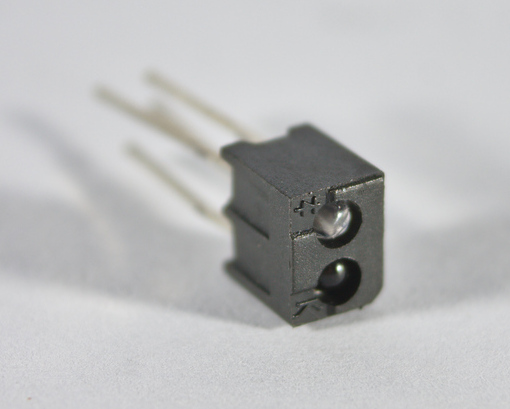
\includegraphics[width=0.9\linewidth]{images/30_proximity_front.jpg}
  \caption{front-view}
  \end{subfigure}
  \begin{subfigure}{0.48\textwidth}
  \centering
  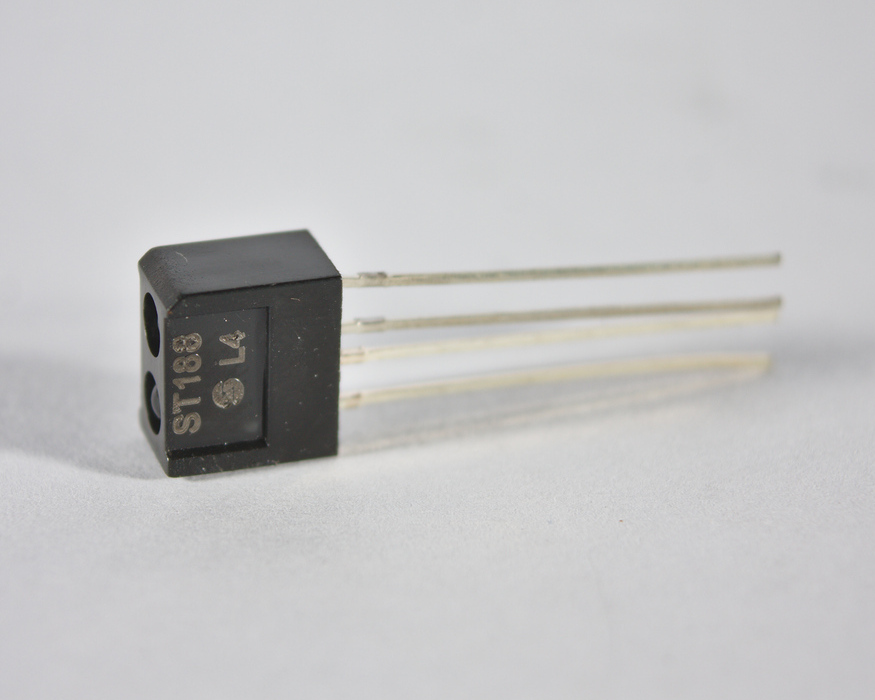
\includegraphics[width=0.9\linewidth]{images/30_proximity_back.jpg}
  \caption{side-view}
  \end{subfigure}
  \caption{IR proximity sensor (CC-BY-SA Ben Oswald)}
\end{figure}

Applications for proximity sensors are line following, edge detection (for instance of a table) or generic brightness measurement. When facing the front of the robot proximity sensors can be used to prevent collisions by measuring the proximity of the surrounding objects.

The price of a single proximity sensor is about 0.5 USD for average quality low distance sensors suitable for the application mentioned before. Microcontroller pin requirements are one pin to enable the infrared led within the proximity sensor (optional) and another analog-to-digital converter enabled pin to perform the readings of the photodiode. When multiple proximity sensors are used within a robot, analog multiplexer 

\subsection{Ultrasonic Distance Sensor}
Ultrasonic distance sensors sense distance between the sensor and an object in the visible area of the sensor. In case of ultrasonic sensors the visible area is the area where the echo spreads. By counting the time between the signal and the reflection the distance can be calculated using the speed of sound (340.29m/s at sea level). 

\begin{figure}[H]
  \centering
  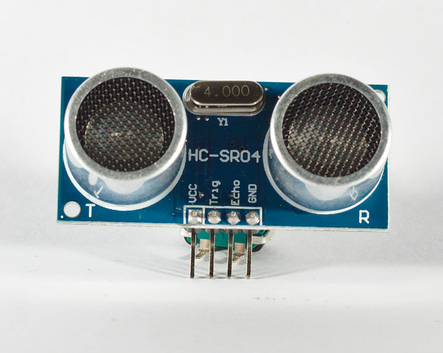
\includegraphics[width=0.5\textwidth]{images/30_ultrasonic.jpg}
  \caption{HC-SR04 ultrasonic distance sensor (CC-BY-SA Ben Oswald)}
\end{figure}

The price for an ultrasonic distance sensor is very low, cheap versions with a range between 1 and 255 centimeters start at about 1.5 USD. Interfacing the sensor requires two microcontroller pins - one for triggering the echo and another one for reading back the distance value. The trigger pin can be a generic purpose input/output pin, the sense pin must be attached to a pin which provides an analog to digital converter.

A typical application for ultrasonic distance sensor is obstacle avoidance. By mounting the sensor on a servo motor the visible area can be increased which allows better navigation due to enhanced obstacle avoidance possibilities. 

\subsection{Accelerometer}
Accelerometers can sense acceleration on one or more axis. This can be used to determine the speed of the robot or the direction in which the robot accelerates (which can be used to determine whether the robot falls/is lifted up). 

Interfacing accelerometer is often done using serial protocols like SPI (Serial Periphal Interface), UART (Universal asynchronous receiver/transmitter) or I2C (Inter-Integrated Circuit). A affordable accelerometer with included gyroscope (evaluated in the section below) is the MPU-6050. It has a price tag of 3 USD and is usually sold on a breakout-board due to its small QFN (quad-flat no-leads) package which is hard to solder manually. 

\begin{figure}[H]
  \centering
  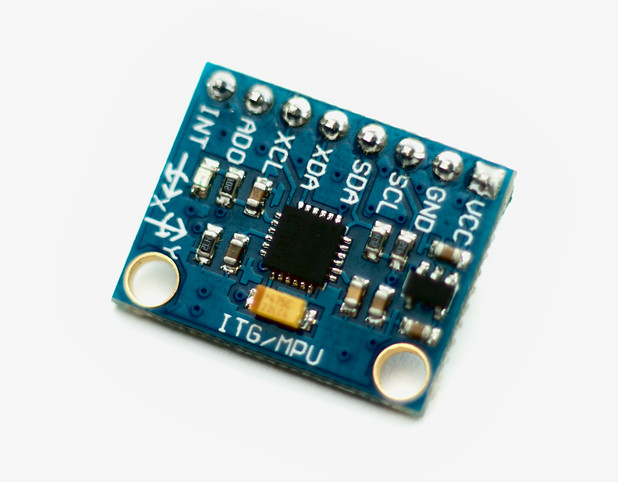
\includegraphics[width=0.5\textwidth]{images/30_gyroaccel.jpg}
  \caption{MPU-6050 breakout board (CC-BY-SA Ben Oswald)}
\end{figure}

The MPU-6050 can be interfaced using various protocols, but I2C is the most common way to do so and requires two input/output pins only using software-based I2C or two I2C hardware pins. Libraries with permissive license exist which ease the use of the accelerometer. For advanced usage scenarios a integrated DMP (Digitial Motion Processor) can process raw values and interface additional sensors like a compass.
\subsection{Gyroscope}
Gyroscopes are used to determine the orientation. Applications for gyroscopes are balancing and position calculation (usually in combination with an accelerometer). Integrated circuits such as the MPU-6050 mentioned before usually combine a gyroscope and an accelerometer into one single device.

The educational potential of a gyroscope/accelerometer is excellent, since interaction with a robot can be directly visualized. It can introduce the user to concepts of orientation and force by interacting with the robot. Advanced users can use the sensor to determine the position in of the robot based on a known starting point or lifting/falling detection.

As mentioned in the previous section the MPU-6050 is easily interfaced using various protocols of which I2C is the common way.
\subsection{Compass}
A compass allows the robot to sense its orientation relative to the magnetic field of the earth. Technically speaking a integrated circuit providing measurement of the magnetic field of the earth are a special form of magnetometers.

\begin{figure}[H]
  \centering
  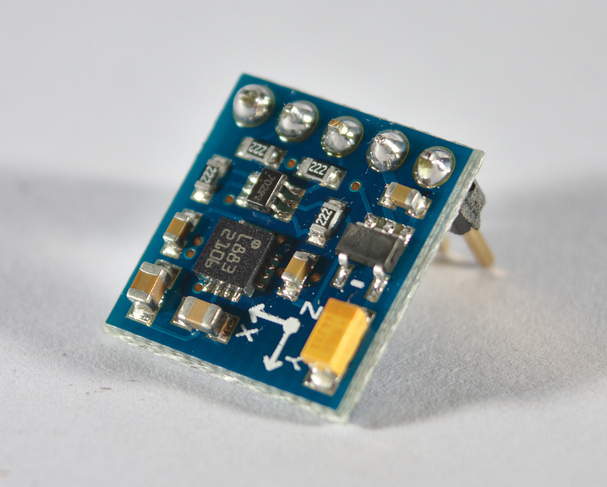
\includegraphics[width=0.5\textwidth]{images/30_compass.jpg}
  \caption{Triple axis compass on breakout-board (CC-BY-SA Ben Oswald)}
\end{figure}

An integrated circuit providing a magnetometer is the HMC-5883L which is interfaced with I2C. It costs about 3 USD and is mounted on a breadboard friendly breakout board. It senses the magnetic field in three axis.


The educational potential of a compass is given since the interaction can be directly measured (typically accuracy is 1 degree). It can be used to introduce the magnetic field of earth and its function. Advanced users can use the compass to navigate the robot with higher precision (in combination with the accelerometer and gyroscope).
\subsection{Conclusion}
Each sensor enables new robot applications such as sensing the environment, movement or navigation. Due to the fact that most sensors are already mounted on a breakout-board, the sensors are accessible to people without sophisticated soldering experience. In addition a robot can be designed to provide connectors for the breakout boards which gives more flexibility.

The flexibility influences the power consumption since only sensors needed for a specific application have to be mounted/enabled. Considering the target audience of the robot, sensors can be bought separately on demand which reduces the costs for the base robot.
\section{Communication}
Communication between robots or between the robot is essential to widen the application possibilities. When the robot is connected to a computer it gets much more processing power to solve complicated problems; when robots can communicate with each other tasks can be solved collaboratively.

\subsection{Infrared}
Infrared based data transfer is widely used in remote control application where a small amount of data, usually a single word, is transferred. Infrared communication is easily interfered by other infrared signals. This limits the data rate since error correction mechanisms must be implemented.

\begin{figure}[H]
  \centering
  \begin{subfigure}{0.48\textwidth}
  \centering
  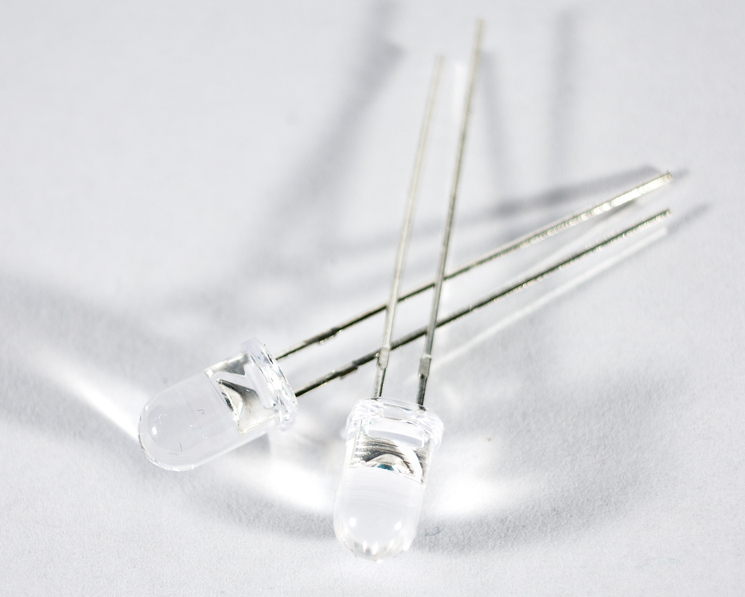
\includegraphics[width=0.9\linewidth]{images/30_irdiodes.jpg}
  \caption{Infrared diode (sender)}
  \end{subfigure}
  \begin{subfigure}{0.48\textwidth}
  \centering
  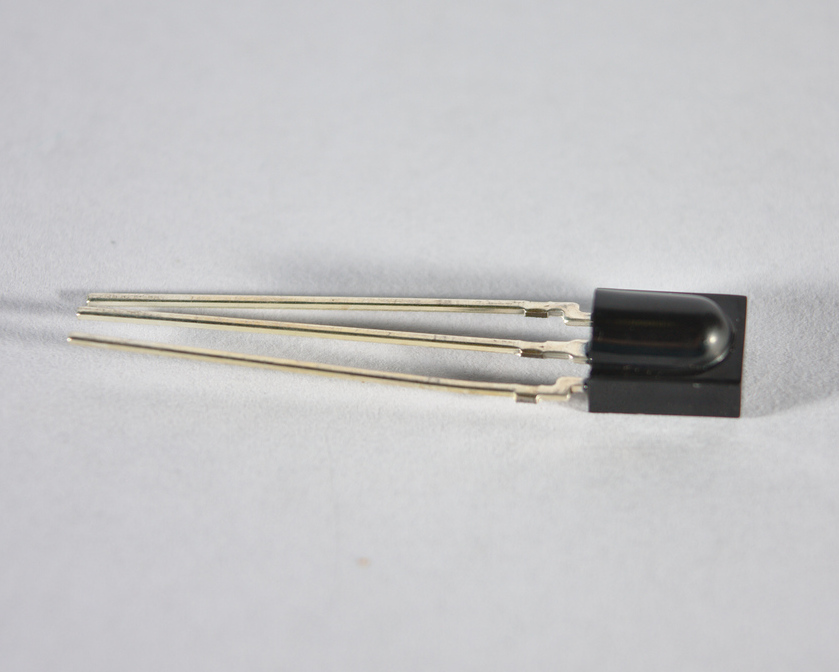
\includegraphics[width=0.9\linewidth]{images/30_ir.jpg}
  \caption{Infrared receiver (reciever)}
  \end{subfigure}
  \caption{Components for infrared communication (CC-BY-SA Ben Oswald)}
\end{figure}

When using infrared signals only one robot can send at a time which requires collision detection. The hardware requirements for infrared transmissions are ver low, only a infrared reciever and a infrared LED is required which sums up to a total of 0.5 USD. The infrared reciever and the infrared LED require one free GPIO pin on the microcontroller each. To ease programming the reciever should be attached to a microcontroller pin which is suitable for external interrupts.

Since a lot of effort is needed to make the connection stable, this solution is not trouble free, although techniques to stabilize communication have educational potential. A standardizes data exchange format for infrared communication does not exist.

\subsection{RFM12B}
The RFM12B is a wireless transceiver operating in the 434MHz or 915MHz band. It is produced by HOPE RF and provides an SPI interface to communicate with a microcontroller. 

It operates at voltage levels from 2.2V to 3.8V and provides data rates up to 115.2kbps. It comes without a breakout board but is shaped with stamp holes which are easy to solder. The price tag is about 7 USD for each module.

The maximum distance depends on the antenna used. A arduino compatible library exists which is licensed under MIT license. Connecting the RFM12B requires four SPI pins (MISO, MOSI, SCK and CS) and an additional IRQ interrupt on an external interrupt pin.
\subsection{NRF24L01}
The nRF24L01 (or its sucessor the nRF24L01+) are single chip trancievers by Nordic Semiconductors which operate in the license free 2.4GHz frequency band. The allow sending and recieving of data and can standby in ultra low power mode consuming 900nA at 3.3V only.

\begin{figure}[H]
  \centering
  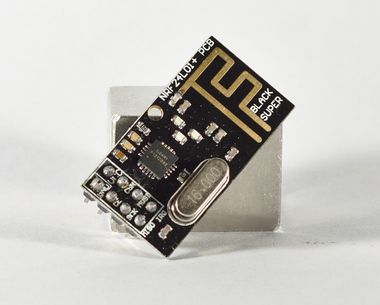
\includegraphics[width=0.5\textwidth]{images/30_nrf24l01.jpg}
  \caption{nRF24L01 breakout board (CC-BY-SA Ben Oswald)}
\end{figure}

Attaching the nRF24L01 to the microcontroller requires four SPI pins (MISO, MOSI, SCK and CS), an additional CE (chip enable) pin and an external interrupt pin to indicate state. Even though the microcontroller runs at 3.3V the inputs are 5V tolerant. The maximum data rate of the module is 2 Mbit/s, lower data rates (1 Mbit/s or 250Kbit/s) increase the maximum distance between two modules.

Two open source libraries Mirf and RF24 exist. RF24 is licensed under a GPL 2.0 license and Mirf is provided under a permissive "as is" license. The price for a nRF24L01 on a breadout-board is around 3 USD on ebay, other modules with external antenna have a higher price tag.
\subsection{Conclusion}
In terms of cost-effectiveness the nRF24L01 is the best solution for wireless communication between robots. The transmission is robust, easy to implement due to library support. Since the chip comes mounted on a breadboard with 2x4 header, a user can populate a socket and add the module on demand.
\section{Microcontroller}
Depending on the microcontroller, the final robot has different processing capabilities. Its capabilities are mainly influenced by the processor frequency which influences the number of instructions per second, the interfaces such as I2C or SPI and the amount of flash storage and RAM.

Since the target audience are beginners, the evaluation focusses on microcontrollers used by the Arduino project which provides libraries and tutorials for a lot of applications. A Arduino community exists where questions are discussed and answered. Those answers can be easily ported to the robot when the underlying microcontroller is compatible with the Arduino bootloader.
\subsection{ATmega328p}
The ATmega328p is a low power microcontroller produced by Atmel which runs on voltages between 1.8 and 5.5 Volt. It is usally operated at 5 Volt with a frequency of 16 MHz. The microcontroller has 32KB of integrated flash memory, 2KB RAM and 1KB EEPROM. Hardware interfaces include a UART, SPI and I2C (called TWI - two wire interface). Six microcontroller pins provide an analog to digital converter with 12 bit resolution (0 to 1024), additional 14 pins are generic input/output pins of which six pins provide PWM (pulse-width-modulation) capabilities.

The ATmega328p costs about 3.5 USD in a single unit, when buying in bulk the price drops to about 2 USD per unit. The microcontroller can be programmed using an ISP (In-system programmer). When the Arduino bootloader is present, the microcontroller can be programmed using its UART. The bootloader consumes about 0.5KB of flash memory. Using the UART for programming requires a USB to serial cable with TTL logic level and reset pin. Integrated circuits such as the FTDI  FT232RL provide this functionality for about 4 USD plus additional components.
\subsection{ATmega32U4}
The ATmega32U4 is a microcontroller produces by Atmel with integrated USB connectivity. It usually operates at 5 Volt with a frequency of 16Mhz. It provides 32KB of flash memory, 2.5KB RAM and 1KB EEPROM. 

Interfacing other hardware components is possible using 20 digital input/output pins of which seven provide PWM output and twelve pins act as an ten bit analog to digital converter. Hardware interfaces for I2C, SPI and UART exist, the USB interface can be used for emulating a serial interface or usb mouse and keyboard.

When the Arduino bootloader is present on the microcontoller it can be programmed using the usb serial device. This reduces the available flash memory by 4KB to 28KB available. It also reduces the need of additional components such as an FT232RL for programming via USB.
The cost per microcontroller is 6 USD for a single unit and drops to 3.5 USD in large quantities.
\subsection{Conclusion}
Both, the ATmega328p and ATmega32U4 are suitable for robotic projects. The pricing is similar considering the microcontroller to be programmable via USB (ATmega328p: 7.5 USD - ATmega32U4: 6 USD). Both microcontrollers well supported in the arduino community and provide sufficient connectivity for sensors and actuators.  

Some features make the ATmega32U4 more favorable than the ATmega328p such as the increased number of PWM capable pins and the increased number of pins with an integrated analog to digital converter. In addition the usb keyboard and mouse emulation offers additional usage scenarios even though usb programming is not available in this mode. The newest Arduino generation (Arduino Leonardo) is based on the ATmega32U4.
\section{Power Supply}
Supplying power to the robot can be archieved using different technologies. Difficulties exist in handling the needed voltages and current for all attached devices including the microcontoller, actuators and sensors. Criteria on which power supply technologies are evaluated are the discharge rate, the cost and of the security.
\subsection{Nickel-metal hydride batteries}
Nickel-metal hydride batteries better known as NiMH batteries are rechargeable with a nominal voltage of 1.2Volt and a energy density of 140 to 300 watt hours per liter. The durability of the cell is often specified in the range of 500 to 1000 charge cycles. Maximum discharge rates are about 1C which means full discharge in one hour.

Special charging circuits exist which ease the charging process. Different charging techniques such as trickle charging (constant low current), $\Delta$ V charching (voltage monitoring) and $\Delta$ T charging (temperature monitoring) exist. Each of method has its own advantages and disadvantages and may be combined.

When NiMH batteries are overcharged the battery cell can destroy the cell by rupture. A vent prevents the cells from busting, hydrogen is emitted when the battery is overcharged. Similar to overcharging the cell can be destroyed by over-discharging. In that process the cell reverses its polarity and therefore good cells start to drive the discharged cell in verse.

Concerning environmental impact NiMH batteries are ready for recycling when disposed into special collecting points. Modern low self-discharge NiMH batteries which provide 2000mAh (AA sized) have a price tag of 2.5 to 3 USD and 2 USD for a 750mAh (AAA sized) battery. 
\subsection{Lithium-polymer batteries}
Lithium-polymer batteries are rechargeable batteries with a nominal cell voltage of 3.7V  and a density of 300 watt hours per liter. The charge cycle durability is over 1000 cycles and the self discharge rate is very low (about 5 percent per month). During charge the voltage increases to 4.2V and drops to 3V during discharge. Therefore voltage stabilizing components such as step-up converter are needed to provide a constant voltage.

\begin{figure}[H]
  \centering
  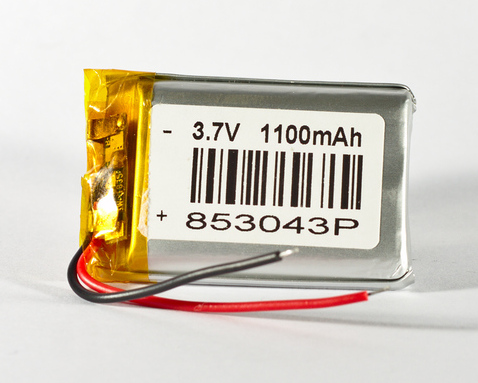
\includegraphics[width=0.5\textwidth]{images/30_lithium-polymer.jpg}
  \caption{Lithium-polymer battery (CC-BY-SA Ben Oswald)}
\end{figure}

There exist special charging circuits which support the charching curve required . The discharge rate can be multiple times the capacity.
To prevent damage due to overcharging, over-discharging and over-discharge-current a protection circuit is integrated into most lithium-polymer batteries.

When overcharging a lithium-polymer battery without protection circuit the battery can cause explosion or fire. When the battery is short-circuited it expands (in volume) and may cause fire. Same holds for opening/damaging the battery. 

Advantages over other battery types exist in energy density and the high cell voltage of 3.7 Volt which reduces the amount of cells needed. The high current during discharge is well suited for driving variable current sources such as DC motors. Its small size and low cost of about 10 USD for a 3.7 Volt 1000mAh cell with a weight of less than 10 gramm is easy to handle.
\subsection{Conclusion}
Even though lithium-polymer batteries expose a greater risk when handled wrong (overcharging, over-discharging and over-discharge-current), they provide higher rated discharge current and a high cell voltage. The size of lithium-polymer batteries is compact and security measures  exist which prevent harm up to a certain extend.
\chapter{Robot Construction}
The design and construction process of the robot is based on the evaluation and evaluation critera. Having the results of the previous evaluation, the design process can focus on the best suited parts.

Components which usage is desired in the robot are: stepper motors with wheels attached for movement, infrared sensor, ultrasonic distance sensor, accelerometer, gyroscope and compass for sensing the environment and lithium-polymer batteries as power supply. Controlling the components and the execution of custom programs should be realized by an ATmega32U4 microcontroller.

\section{Electrical requirement}
Each component has its own electrical requirement such as voltage, current and pin count. The requirements for all components can be added up to create a power supply and a wiring concept. 

\begin{description}
\item[Stepper motors and driver] \hfill \\ The 28BYJ stepper motors are specified for usage with 5 volt. It is possible to drive the motors with lower voltage but rotation speed and torque suffer under lower voltages. Typically for motors, the current varies depending on the coil position and the magnetic field applied. Empirical experiments show, that the maximum current flow in the stepper motors and the driver is 140mA (at 5V) each when the motor is stuck and cannot rotate.\footnote{Measured using a multimeter with hold-on-peak mode between the supply GND and VCC. Rotation was blocked by holding the shaft with one hand.} During normal operation the current flow is between 40 and 100mA (at 5V). It is safe to assume, that the maximum current for the stepper motors and the driver chip is 300mA at 5V.
\item[Microcontroller] \hfill \\ The ATmega32U4 works at various supply voltages from 2.7 to 5.5V. According to the datasheet, the frequency is limited with lower voltages. To support 16MHz operation, the voltage must be between 4.5 and the maximum voltage of 5.5V. The current consumption with this speed is between 10 and 14mA.
\item[Ultrasonic proximity sensor] \hfill \\ The ultrasonic proximity sensor runs with a nominal voltage of 5 volt. The working current is 15mA, the idle current below 2mA according to the datasheet.
\item[Infrared sensor] \hfill \\ The infrared sensor is based on a photodiode and a infrared LED. When in use the LED consumes up to 20mA (at 5V) 
\item[Accelerometer and Gyroscope] \hfill \\ The MPU-6050 can operate with 3.3V or 5V due to an integrated voltage regulator on board. At 3.3V the IC consumes 0.5mA for the accelerometer and 3.6mA for the gyroscope (according to the datasheet). Considering the supporting elements like voltage regulator, a total current consumption of less than 10mA can be assumed.
\item[Compass] \hfill \\ The HMC-5883L operates at 3.3V and has a typical current draw of 0.1mA according to the datasheet. Since the breakout board has it's own voltage regulator, the current draw is a bit higher.
\item[NRF24L01] \hfill \\ According to the datasheet the NRF24L01 consumes up to 13.5mA during communication at 3.3V and when in idle only 900nA at the same voltage level.
\end{description}

All in all the brief power consumption sums up to approximately 380mA at 5V and 15mA at 3.3V when all components run at their peak current. According to the Arduino reference\footnote{\url{http://arduino.cc/en/Main/arduinoBoardUno}}, the 3.3V port provides 50mA for shields and therefore the 3.3V supply should provide at least 65mA. The maximum output current for the 5V pin is not specified but can be estimated by looking at the components on an average Arduino board:

The power supply for each Arduino based board is limited by a fuse which cuts the power supply when more than 500mA is drawn from the power source. Given that value, the maximum current available is 500mA at 5V. The available current is reduced by microcontrollers, LEDs, power regulator and other parts that dissipate power. In case of the Arduino Uno board\footnote{see schematic \url{http://arduino.cc/en/uploads/Main/arduino-uno-schematic.pdf}} the ATmega8U2 consumes up to 14mA at 5V \footnote{see \url{http://www.atmel.com/images/doc7799.pdf} fig. 27-1}, the ATmega8 is rated at 25mA\footnote{see \url{http://www.atmel.com/images/doc7799.pdf} fig. 119}, the power consumption fo the four status LEDs and the LP2985-33 voltage regulator are unknown. Therefore it is safe to assume, that 400mA can be provided by the 5V pin.

This leads to overall an power requirement of 780mA at 5V and 65mA at 3.3V.

\section{Power Management}
Having the power requirements specified as 780mA at 5V and 65mA at 3.3V, the power subsystem can be build.  Since the chosen power source are lithium-polymer batteries, their characteristics have to be taken into account as well.

Lithium-polymer batteries have a voltage range from 3 to 4.2 Volt. The voltage decreases during discharge following a $-x^3$ type function. For the 3.3V power supply a Low-Dropout Regulator can be used which reduces the voltage. When voltages under 3.3V occur, the regulator does not work anymore. At voltages below 3.3V the battery still as 10 to 20\% of its capacity. Therefore a LDO should be supplied by a stable voltage which is constantly higher than 3.3V.

To feed the 5V supply a circuit is needed which increases the voltage range to constant 5V. A boost converter (sometimes called step-up converter) can be used to achieve this. The basic principle of a boost converter is that a capacitor is charged with a higher voltage than the supply voltage by generating a current flow through a diode and an inductor. 

Since the rough power requirement is 1A at 5V, the MCP1650 is a well suited boost converter. If the system is connected to an USB port the boost converter is not needed and should by bypassed. Since automatic switching requires parts which are either available in very small form factors only or consist of complex circuitry, a simple switch is used instead.

\begin{figure}[H]
  \centering
  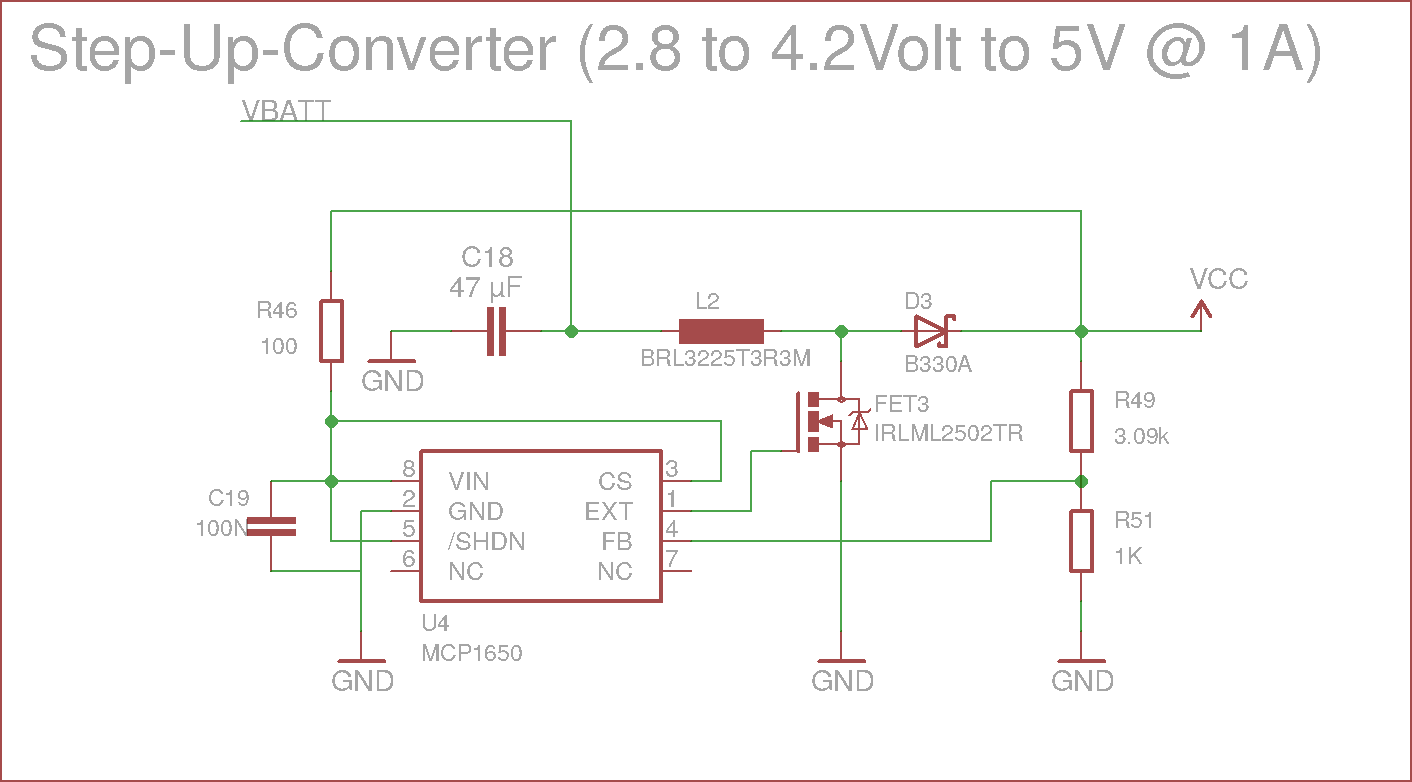
\includegraphics[width=\textwidth]{images/schematic/stepup.png}
  \caption{Stepup converter schematic using the MCP1650}
\end{figure}

For charging the Lithium-Polymer battery a special integrated circuit can be utilized. The MCP73831 is such an IC with programmable output current up to 500mA. A indicator LED attached to one pin of the charge IC gives feedback of the charge status.

\begin{figure}[H]
  \centering
  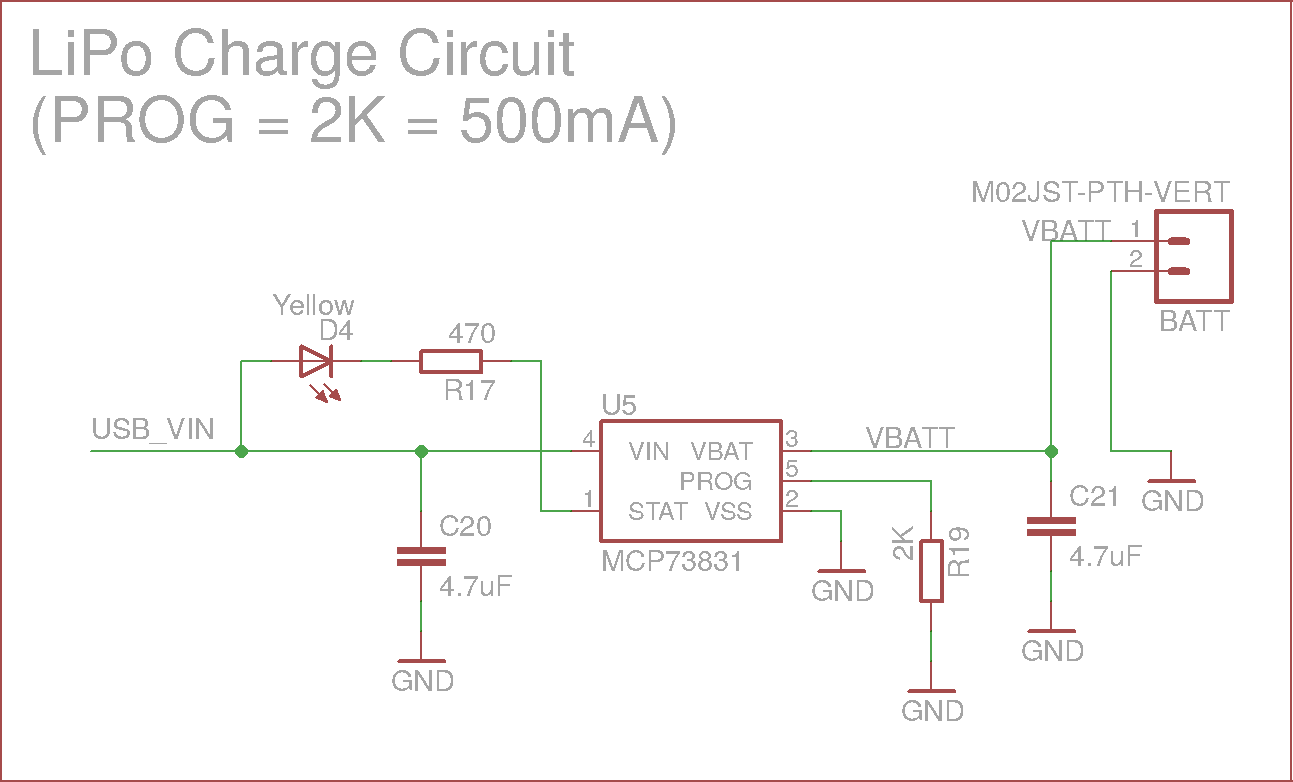
\includegraphics[width=\textwidth]{images/schematic/charge.png}
  \caption{Lithium-polymer battery charge circuit using the MCP73831}
\end{figure}

To switch between battery power and USB power, a simple toggle switch is used. When the switch has the USB position the USB power source powers both the robot main circuitry and the battery charger. When the toggle switch has the battery position, power is drained of the battery.

\section{Processing Unit}
As previously mentioned, the processing of user and sensor data is should be realised using an ATmega32U4 microcontroller. In previous case studies the interfacing requirements of each sensor were evaluated. Having this information, the connections between sensors and the microcontroller can be made.

Hence Arduino compatibility is desired to enable support by a huge community and the use of existing comprehensive hardware tutorials, the typical Arduino Pin Headers should be available to users. Having one ATmega32U4 only makes it impossible to have fully compatible Arduino headers on board, since most pins would be dual used  - by the Arduino sheet and the robots components. Therefore a solution is needed where the headers as well as the robots can be interfaced simultaneously.

Possible solutions are either port multiplexer or another microcontroller which communicate with each other. Port multiplexer (or demultiplexer since they mostly work as output and input) like the 74HC4051 enable the multiplexing of input and output ports. Having three control ports on a eight bit multiplexer enables the selection between the multiplexers ports ($2^3$ combinations = 8 bit). Depending on the selection the selected pin is mapped to one of the microcontrollers pin. If only output pins are needed, shift registers like the 74HC595 can be used. Shift registers work like one-way multiplexers.

Multiplexers have the advantage of being low priced but reduce the number of available pins on the Arduino pin header since there aren't no unused pins on the microcontroller. In addition setting the control lines requires additional CPU cycles\footnote{CITE ME HERE; possible links: http://web.archive.org/web/20130513161312/http://jeelabs.org/2010/01/06/pin-io-performance/ and http://billgrundmann.wordpress.com/2009/03/03/to-use-or-not-use-writedigital/} which may result in a bottleneck. 

Another option is to use a second microcontroller attached to the main microcontroller using some kind of communication protocol. The ATmega32U4 has built in UART, SPI and I2C (introduced as Two Wire Interface, short TWI which is compatible to I2C) which are candidates to be used for communication. In this scenario the main IC sends requests to the second IC which acts as a slave.

The standard UART usage assumes the presence of two communicating parties. The transfer speed is up to 115.200kBit/s with a duty cycle of 8.68us. Disadvantages of using the UART for communication is, that the number of communicating microcontrollers over the same lines is limited to two by default. If the UART is built as a ring, additional processing overhead is introduced. 

SPI can be faster than UART and supports an arbitrary number of participants but requires a chip-select pin for each participant. This is a disadvantage when dealing with pin count issues.

I2C is a bus which works with two lines (SDA and SCL) only. The protocol defines one participant to be the master device, the other devices must act as a slave device. The maximum data rate supported out of the box is the 400kbit/s fast mode. Since no additional pins are required and multiple participants are supported, I2C is the best suited communication system.

The main drawback of using an additional microcontroller is the high price compared to multiplexer based solution. An advantage are the additional capabilities of microcontrollers since additional pins may support hardware PWM, analog to digital converter and hardware interrupts.  

The robot constructed will feature two microcontroller where one acts as the master and the other as the slave device. The master is fully compatible to the Arduino Leonardo and provides Arduino headers for shields. In addition an extended header is included to match the standard 2.54 inch prototyping board. Communication between the microcontroller is realized using I2C. The second microcontroller controls sensors, movement and optional components such as networking. The schematics are in the appendix. A 

Having this setup the user is flexible and can utilize all Arduino possibilities. For advanced users the second microcontroller allows to dive into topics like inter-process-communication, remote procedure calls and distributed computing.  

\section{Optional components}
Due to unused pins on the second ATmega32U4, additional components can be added to the robot platform. Those additional components should add features, have educational potential and should be cost effective. In addition those optional components may be used to generate a profit margin if the robot is produced for educational purposes.

\subsection{Display}
Displaying information and visual feedback helps to debug and reconstruct processes. A cost effective display solution is a standard 1.8 inch TFT display with integrated SD card reader. It is compatible to the Arduino TFT display and integrates the ST7735S display controller. Connecting the display requires standard SPI header and some additional pins. Since SPI is already used to interface the NRF24L01 module, only a chip-select, reset and a data/command switch are needed. The integrated SD card reader needs an additional chip select pin.

\begin{figure}[H]
  \centering
  \begin{subfigure}{0.48\textwidth}
  \centering
  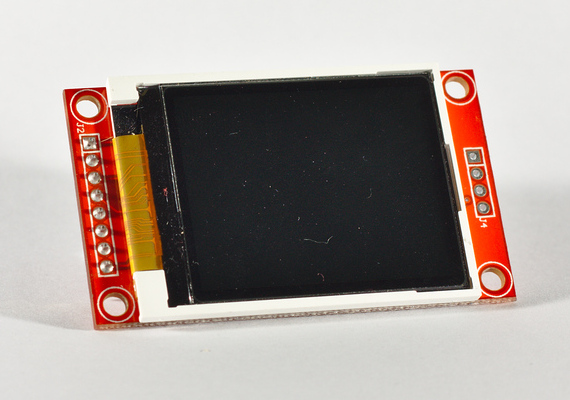
\includegraphics[width=0.9\linewidth]{images/30_tftfront.jpg}
  \caption{front-view}
  \end{subfigure}
  \begin{subfigure}{0.48\textwidth}
  \centering
  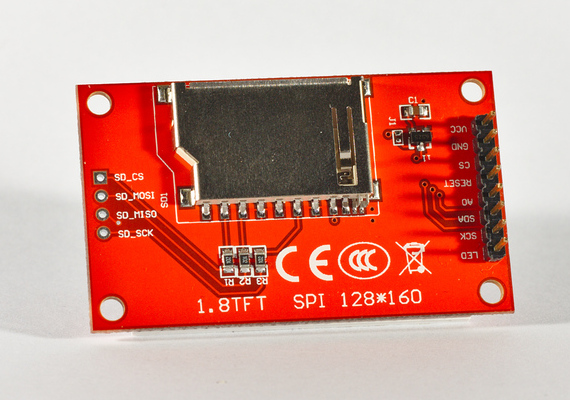
\includegraphics[width=0.9\linewidth]{images/30_tftback.jpg}
  \caption{back-view}
  \end{subfigure}
  \caption{1.8 Inch TFT display (CC-BY-SA Ben Oswald)}
\end{figure}


The display has a display resolution of 128x160 pixel with support for 262000 colors. With an average price of 4.50\euro\footnote{See BOM for optional parts in the appendix.} it provides a lot of features for a low price. Due to its compatibility to the Arduino TFT, the Arduino TFT library can be used.

Power requirement for the display are 30mA at 3.3V for the backlight and 1mA at 5V for the processing unit according to the datasheet\footnote{\url{http://www.adafruit.com/datasheets/JD-T1800.pdf}}. Having a power subsystem which has spare power of 400mA at 5V and 50mA at 3.3V the display can be safely used.

\subsection{Gripper}
Interaction with the real world except movement requires mechanical structures which allow to interact with objects. A gripper is such a mechanical construction which allows to grip and release objects.

A typical Gripper is moved using a servo motor and contrarotating gears attached to it. The contrarotating gear enables the gripper to perform a grip and release action. The typical range of 180 degree for a servo motor, represents the typical range needed for grippers to work. 

A well suited gripper is the Robotic Claw by Maker named Kepler\footnote{see \url{http://www.thingiverse.com/thing:18339/}}. The 3D printed components are simple, robust and relatively cheap to produce. In combination with the Servo motor the costs are 2.04 Euro for the servo and about 0.20 Euro for the 3D printer filament.

\begin{figure}[H]
  \centering
  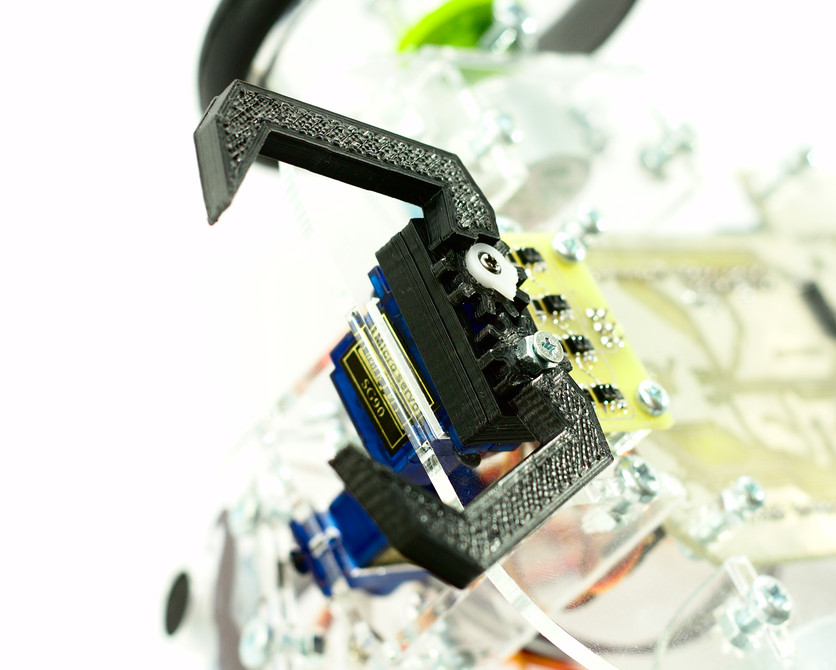
\includegraphics[width=0.8\textwidth]{images/30_gripper.jpg}
  \caption{3D printed gripper mounted on the Robot (CC-BY-SA Ben Oswald)}
\end{figure}


\section{PCB design} 
A PCB (short for printed circuit board) is a non-conductive base material with conductive traces connecting electrical components. Electrical components like resistors, microcontrollers or other integrated circuits are soldered to the traces. Components are available in different types, where THT (Through-Hole-Technology) components have the leads soldered to the opposite site through a hole and SMT (Surface-Mount-Technology) components have the leads soldered at the same side. The following illustration shows the difference between both technologies:

\begin{figure}[H]
  \centering
  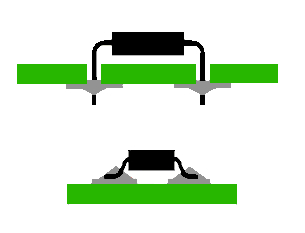
\includegraphics[width=0.7\textwidth]{images/part_types_thtsmt.jpg}
  \caption{Illustration of THT (top) and SMT (bottom) parts on a PCB (green) with Solder (grey) (own illustration)}
\end{figure}

PCBs can have multiple layers with copper traces which are connected using vias. A via is hole made conductive using the process of electroplating. If a PCB contains more than one layer, it is likely that vias are used. Leads of THT components can be used as vias as well, since the hole drilled for the lead is usually electroplated as well.

Before a PCB can be created, a schematic must be drawn. A schematic defines the connections between each pin and therefore gives an overview where electrical connections must be made. The schematic for the robot is found in the appendix. It was made using Cadsoft Eagle - a cross platform CAD program for schematic and PCB layout.

When creating the PCB from the schematic, the schematic must be checked for errors first. EAGLE has a Electrical Rule Check (ERC) built in, which performs several checks such as checks for whether each pin has a connection or checks for power pin connections to power lines. In the board view of Cadsoft EAGLE where one can design the PCB, all components are ordered by their appearance beneath the circuit board first.

The main task is to order the components on the PCB, route traces between pins and keep some basic design rules/guidelines:

\begin{itemize}
\item The width of a trace determines its resistance. The thinner the trace the higher is the resistance and therefore it can carry less current or will heat up. The minimum trace width for a manufacturer is usually 6mil (1 mil = 0.001 inch), homemade etched PCBs are limited to a minimum width of about 10-12mil.
\item The polarity of components is important. For ordinary parts include the symbol for pin one and for diodes and polarized capacitors the plus sign on the silkscreen or the copper layer. This eases manual assembly and prevents errors. \cite[p. 837]{horowitz1989art}
\item Traces and pads (place where a lead connects to) should not be placed to close to each other. Soldering is difficult on close traces and pads. 
\item Sharp edges (angle bigger than 45 degree) are considered bad style. If the angle looks like a "v", problems during the etching process may occur. \cite[p. 837]{horowitz1989art}
\item A ground plane (covering with whole pcb with a ground layer) is good to prevent signalling errors. \cite[p. 456]{horowitz1989art}
\item Components on screen may look bigger than they are in reality. Adding extra space between components makes them easier to solder. The solder tip should not touch other components.
\item Orientation of components should be equal among equal parts to prevent errors while soldering. This especially holds for polarized parts.
\item Due to the target audience all components should be super-sized. Resistors and capacitors should have the 1206 footprint (3.2 mm x 1.6 mm) which can be easily soldered by beginners. For diodes, crystals and integrated circuits the biggest SMD package available at distributors should be chosen. Biggest package not only refers to the package size but also on the spacing between the pins which should be as high as possible.
\end{itemize}

Based on these guidelines the PCB is created. At first the components of the Arduino Leonardo compatible unit (first CPU/user CPU) are layouted. Special care is taken with the spacing between the Arduino shield compatible pin headers. The USB connector for the IC is placed near the edge of the board to allow a good fit for the cable.

\begin{figure}[H]
  \centering
  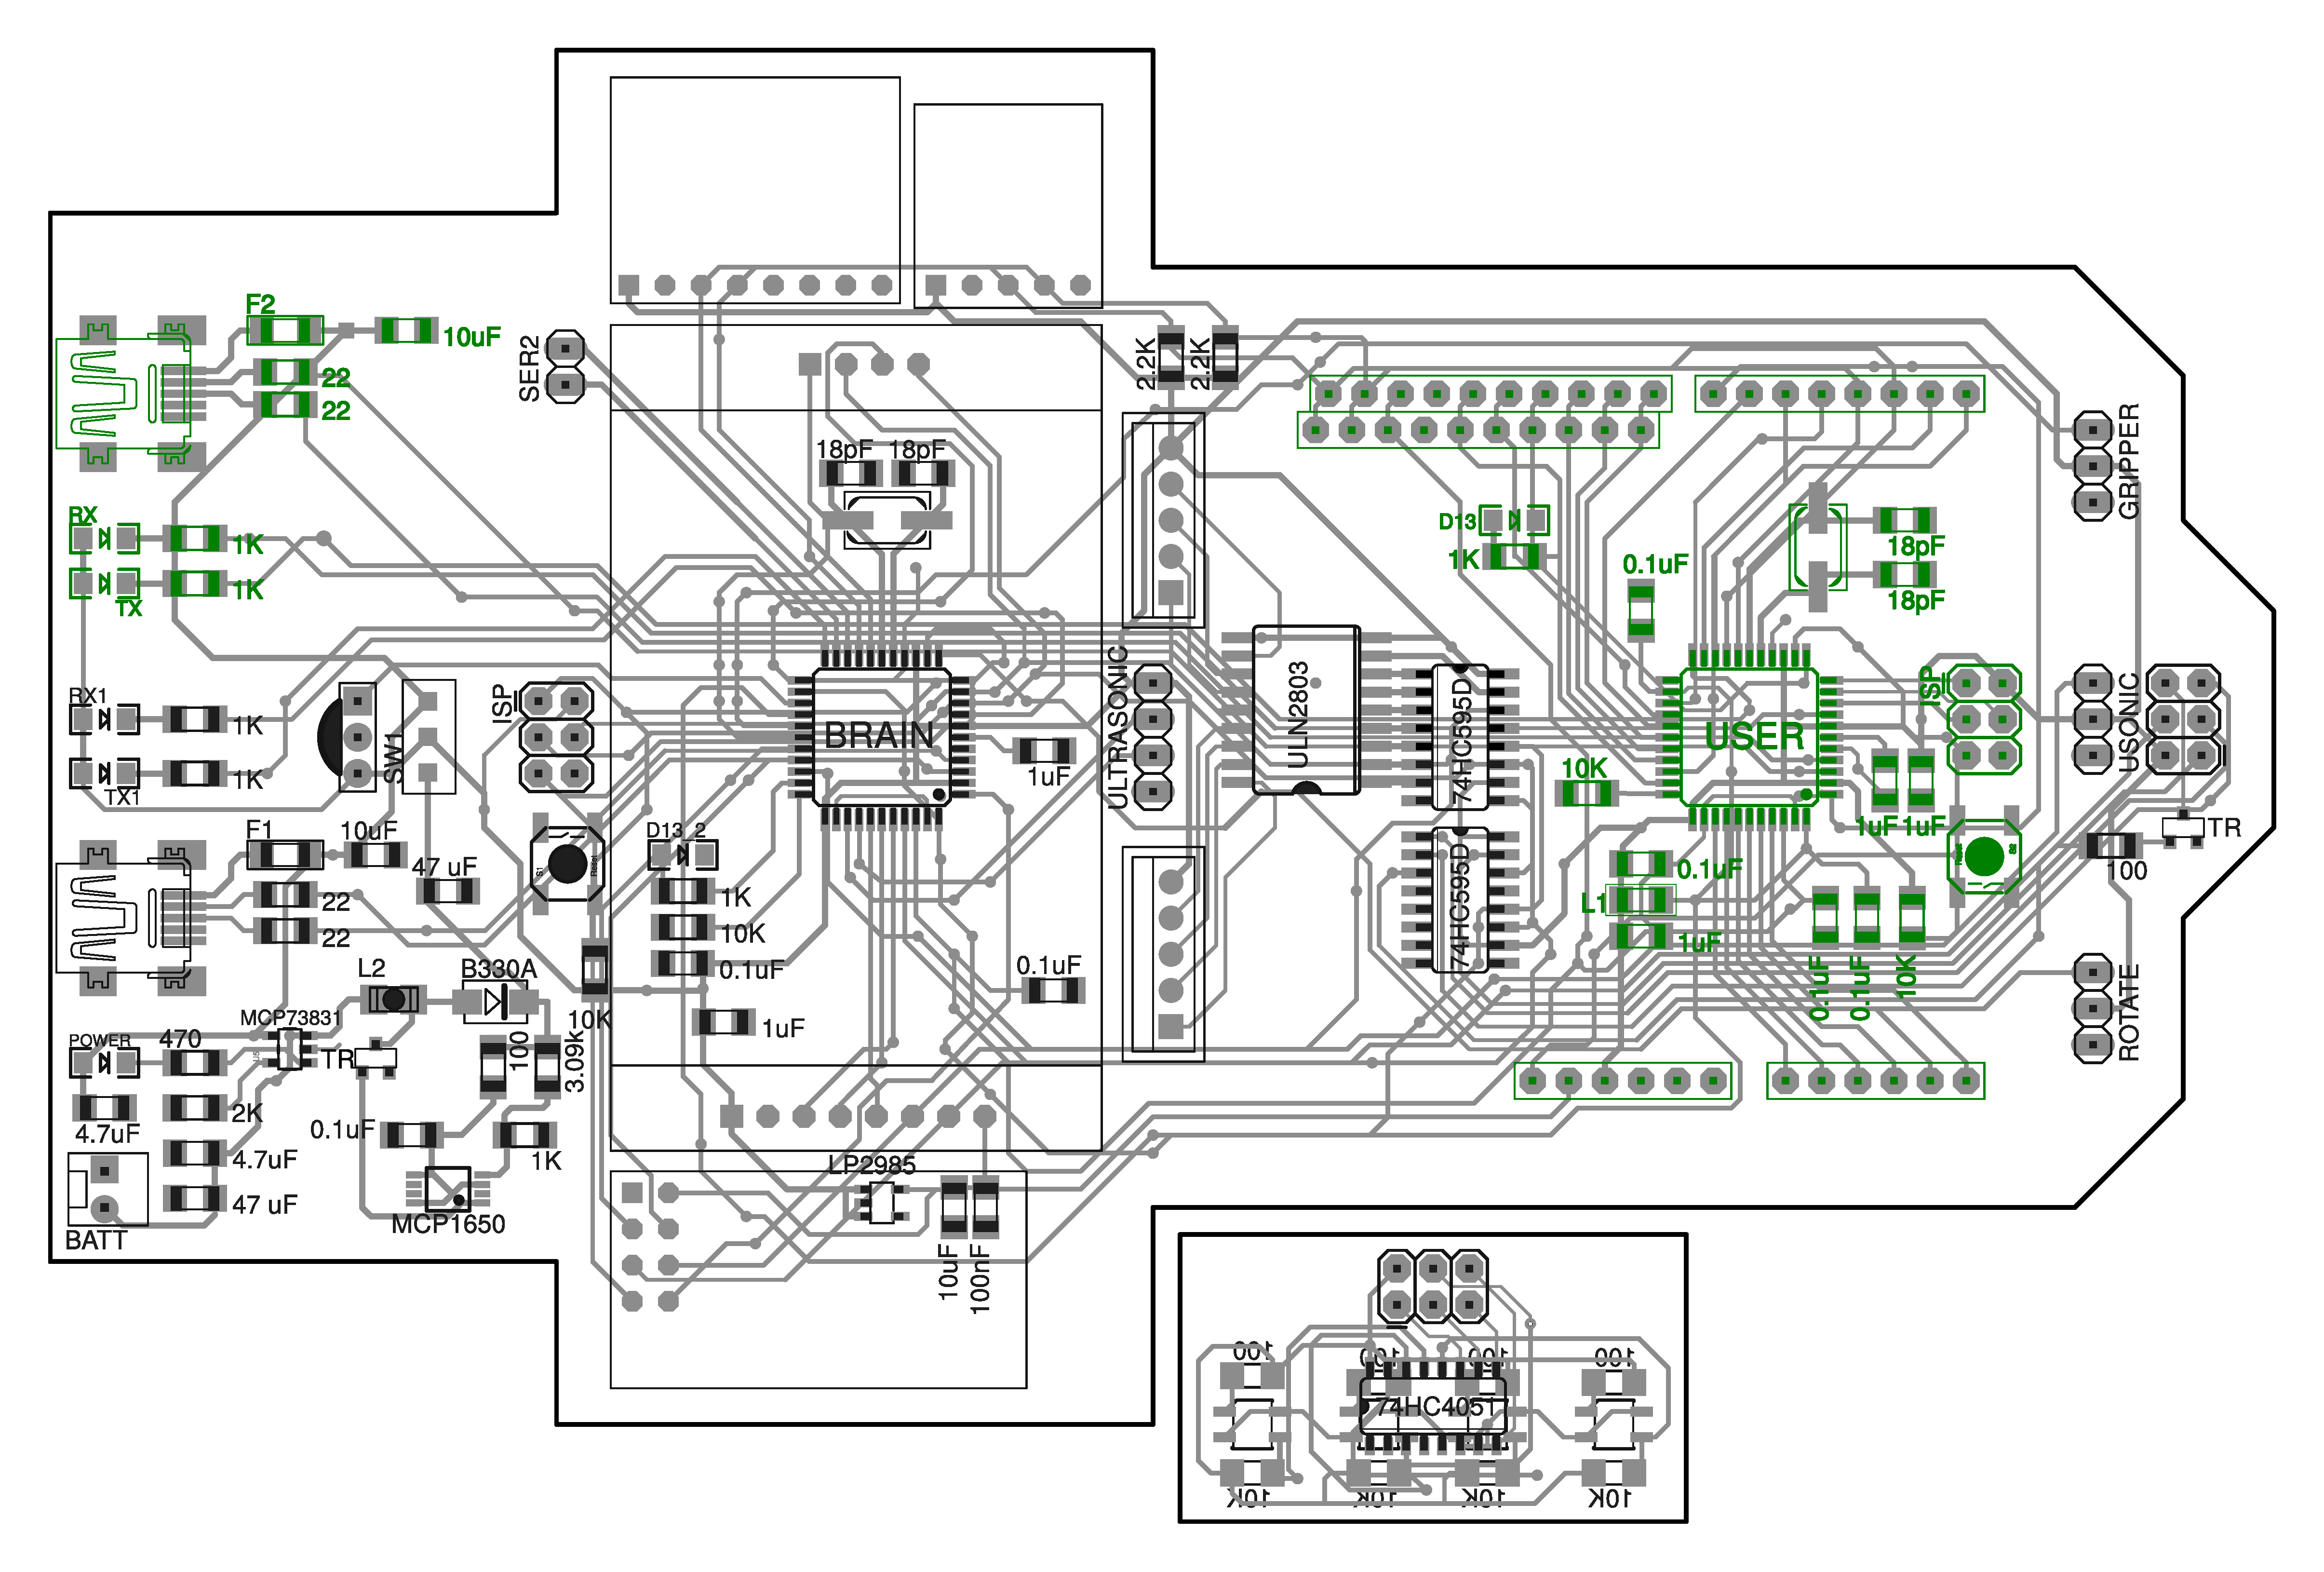
\includegraphics[width=\textwidth]{images/schematic/robot_schematic_user.pdf}
  \caption{Robot schematic creation. Arduino Leonardo compatible circuit part is higlighted in dark green.}
\end{figure}

The next step is to place logically connected components together. The battery charging circuit components are placed near the edge for a good placement of the batteries JST connector. Placing the connector in the middle of the board makes it difficult to carry the battery.

When routing power circuits it is important to set the right trace width. A trace with 10 mil width on 35 micrometer copper can carry up to 1A but heats up 30 degree kelvin. A 20 mil trace only heats up 10 degree kelvin when carrying the same load. \cite[p. 841]{horowitz1989art} 

In the robotic platform developed the trace width for power lines is 16 mil. The expected heat up is tolerable since in normal operation the average current should be much lower.

\begin{figure}[H]
  \centering
  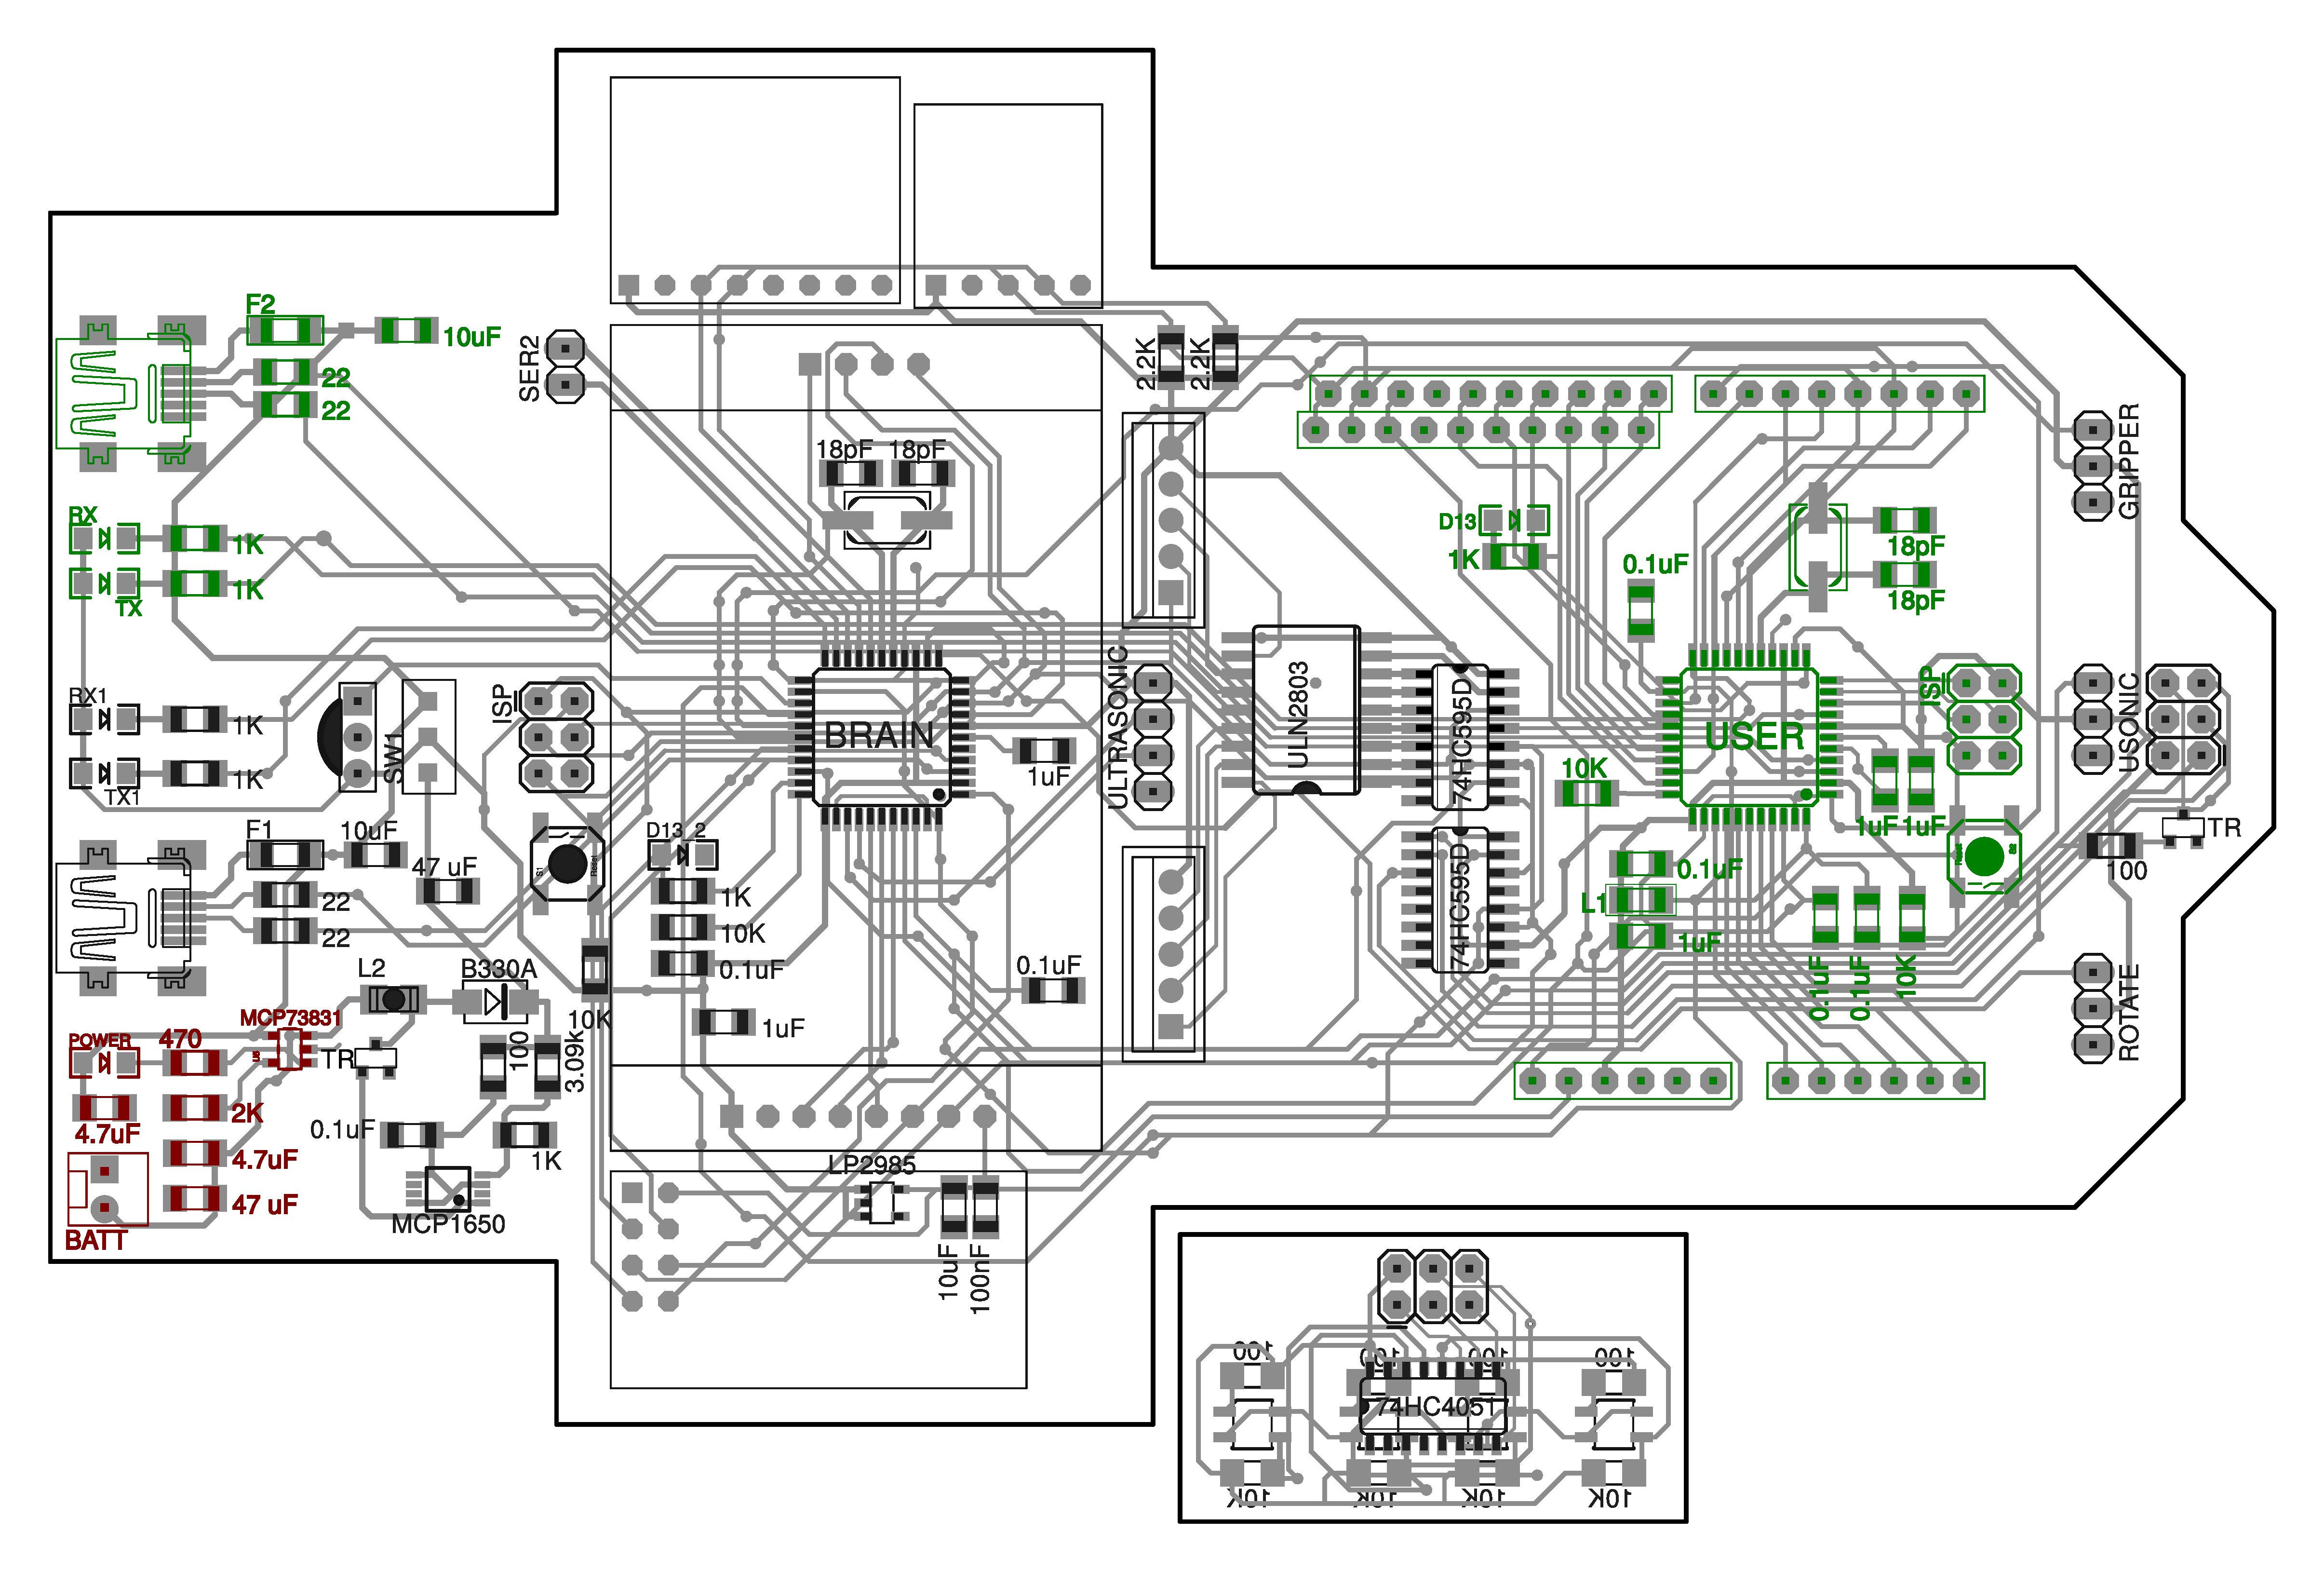
\includegraphics[width=\textwidth]{images/schematic/robot_schematic_battery.pdf}
  \caption{Robot schematic creation. Battery charging circuit components are higlighted in dark red.}
\end{figure}

Followed by the step-up circuit parts most of power related components are placed on the board. The components are placed near the battery charging circuit to reduce the length of the circuits. All components are placed with enough spacing to make soldering easier. This specially holds for the MCP1650 since the leads have a spacing of 0.65mm only. Making this chip easy accessible for desoldering wick helps to re-position it in case of misplacement. 

\begin{figure}[H]
  \centering
  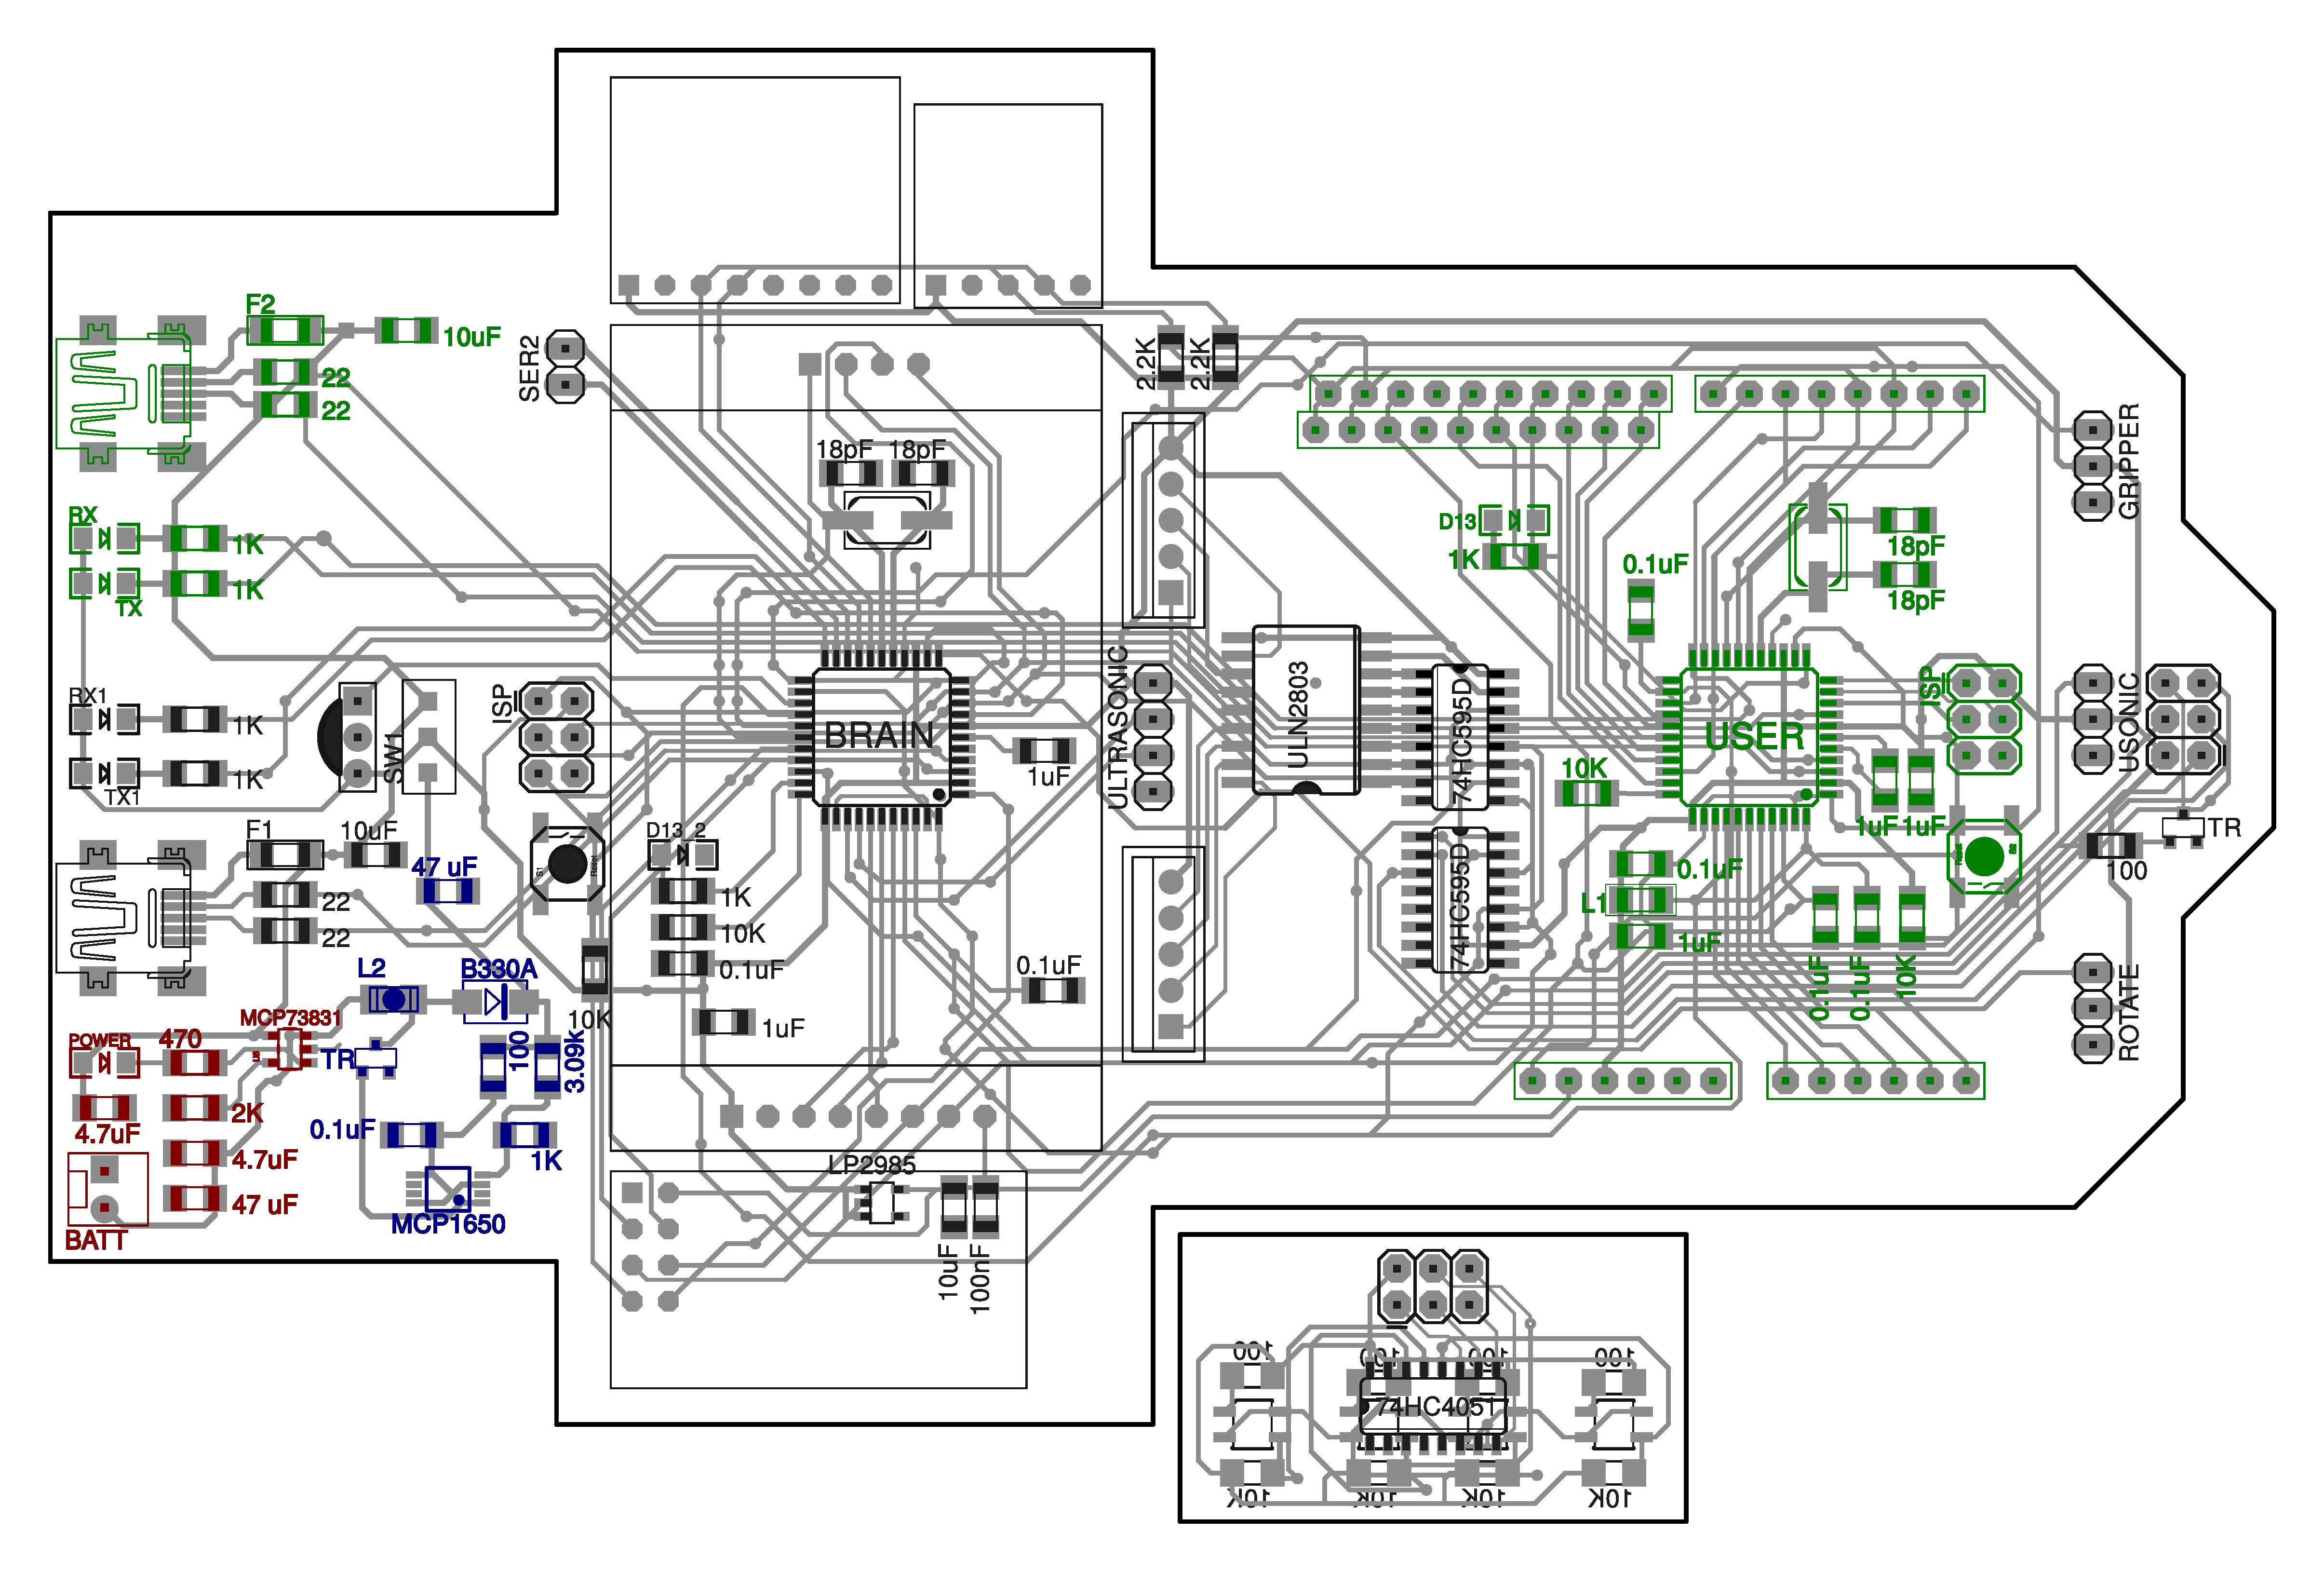
\includegraphics[width=\textwidth]{images/schematic/robot_schematic_stepup.pdf}
  \caption{Robot schematic creation. Step-Up circuit parts are higlighted in dark blue.}
\end{figure}

The 3.3V LDO is mainly for providing power to the optional TFT display, the NRF24L01 module and shields which harvest energy from the 3.3V pins at the shield connector. To reduce the loss of energy due to trace-length the components are placed near the mentioned parts. To stabilize the current flow additional capacitors are placed on the output pins. 

\begin{figure}[H]
  \centering
  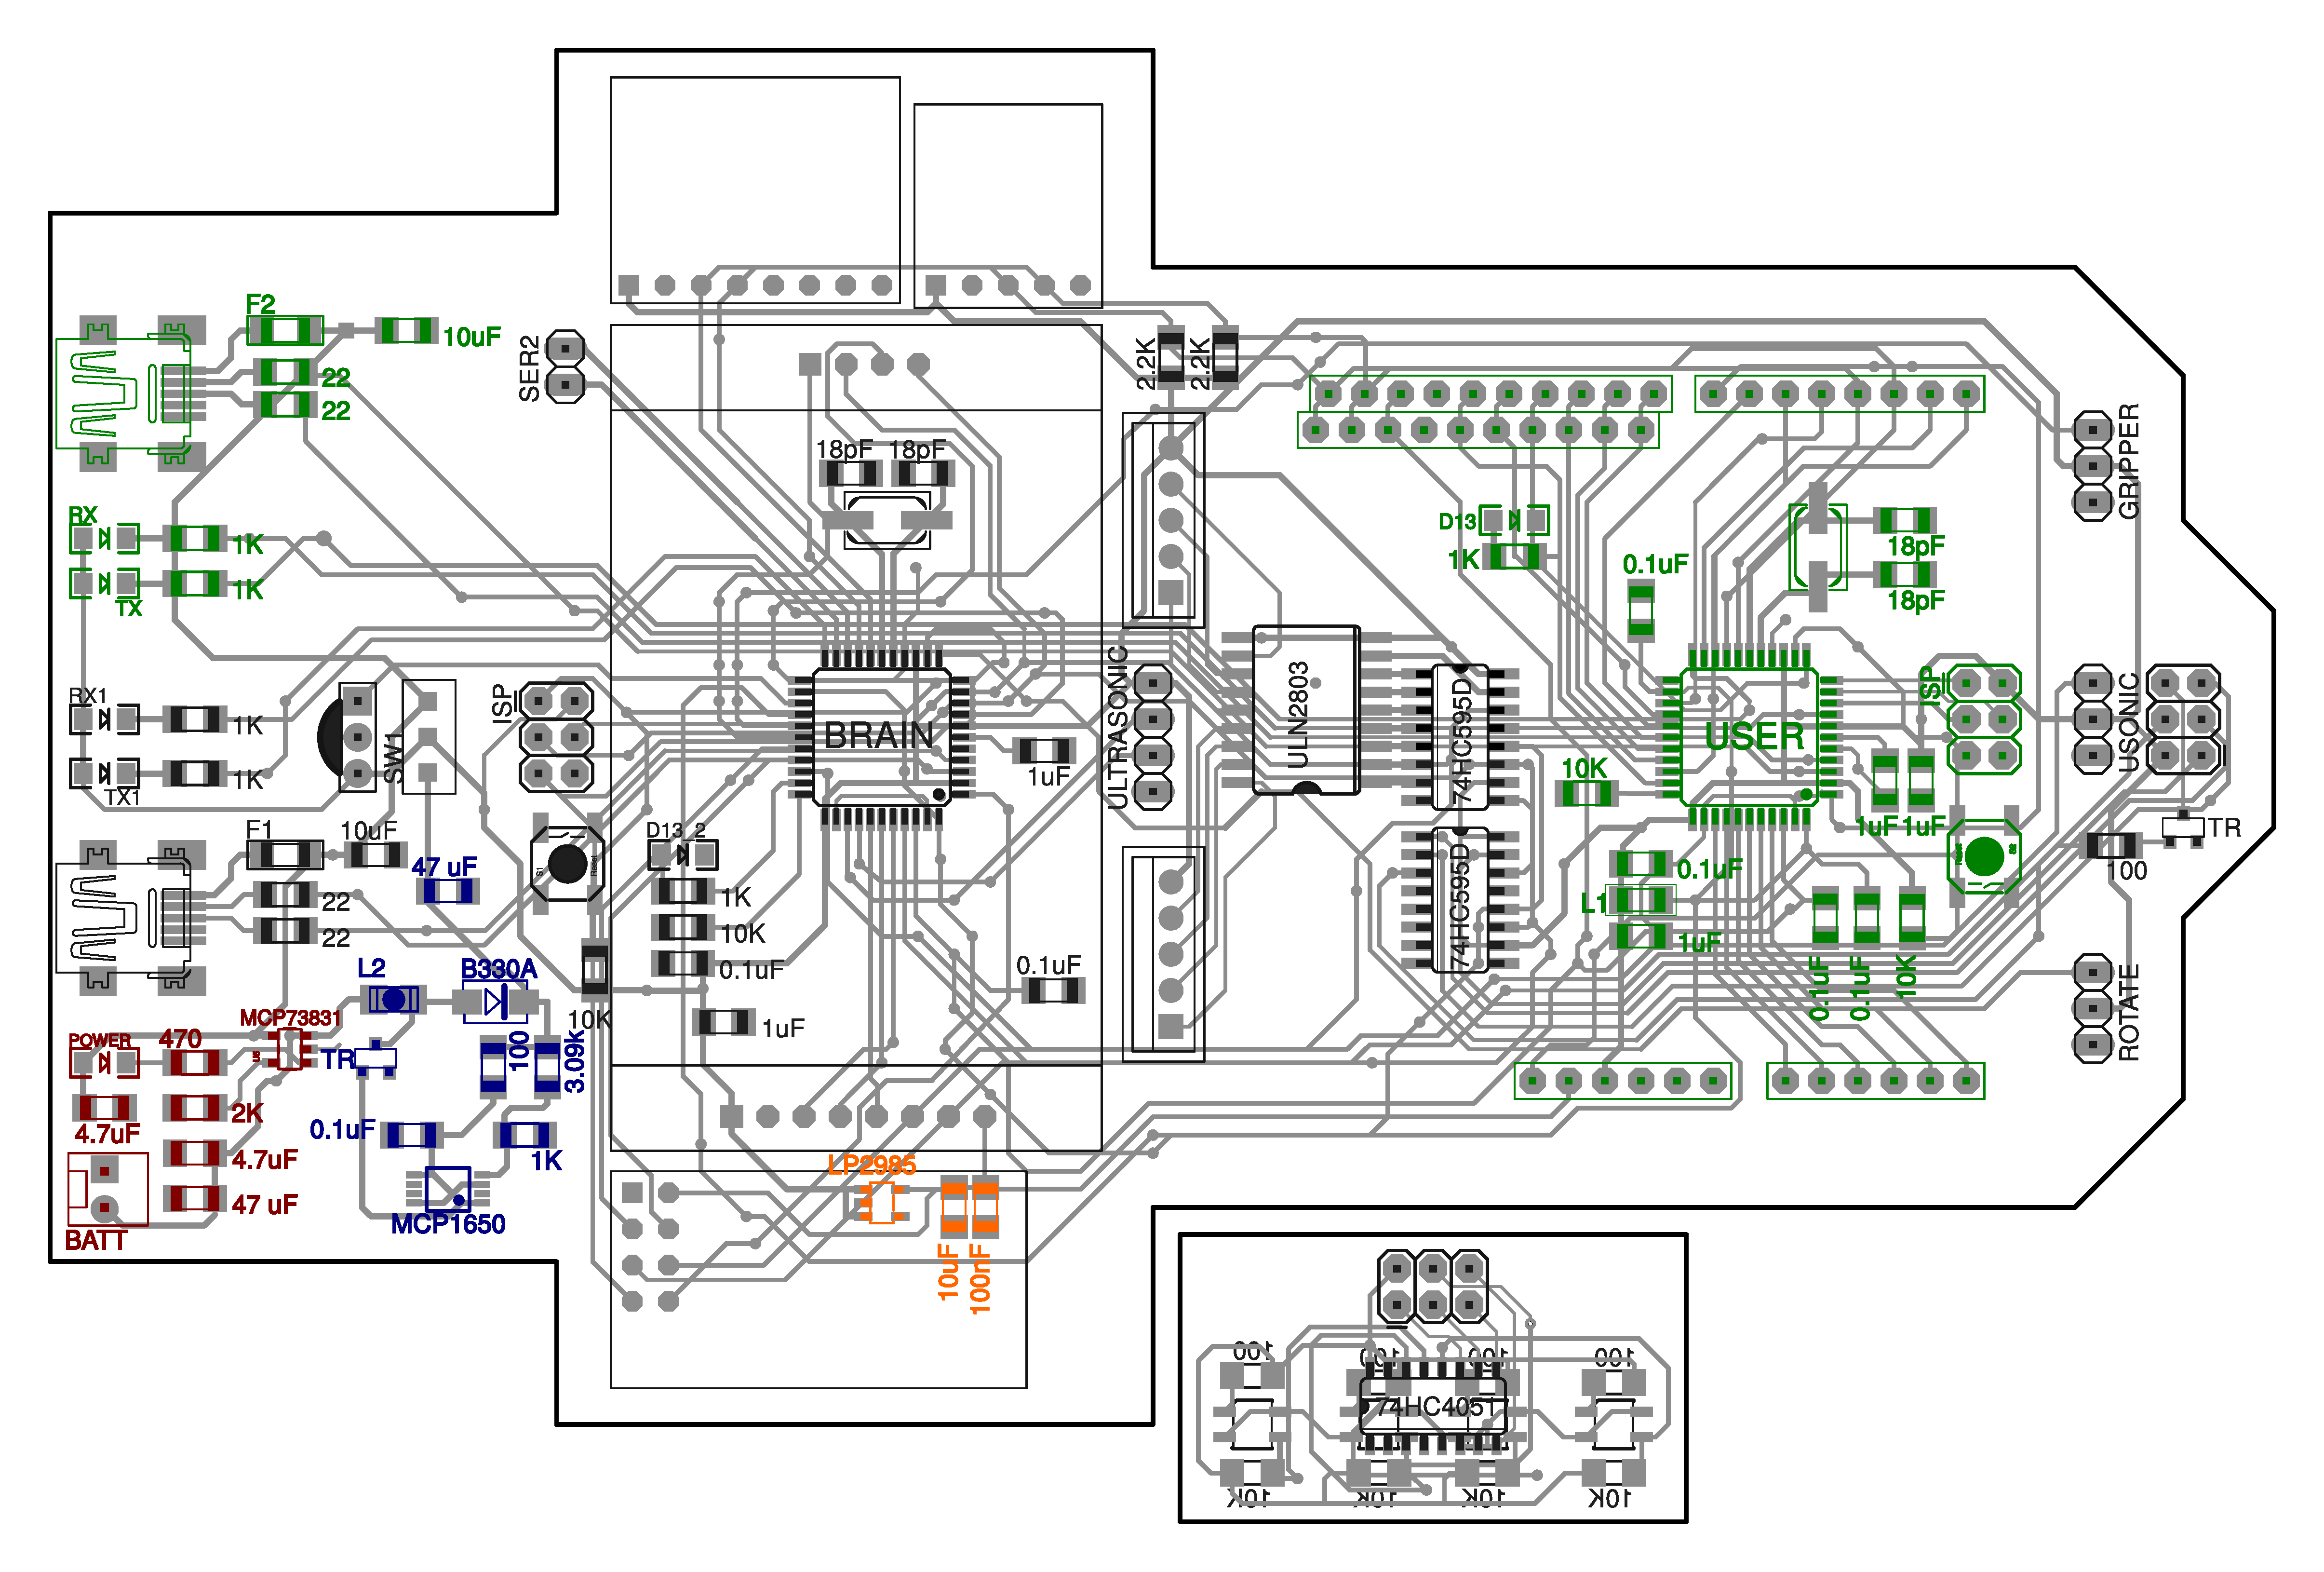
\includegraphics[width=\textwidth]{images/schematic/robot_schematic_3_3v.pdf}
  \caption{Robot schematic creation. 3.3V LDO components are higlighted in orange.}
\end{figure}

Having all power related components placed on the board, the second Arduino Leonardo compatible circuit for controlling sensors, actuators and optional modules is placed on the board. The arrangement of the traces is difficult in this step since the ground-plane on both sides might be interrupted or has orphaned areas. Connecting orphaned ground areas (ground areas which are not connected to ground) can be usually done by placing a via on the orphaned area since the board is designed to be two sided and therefore likely has a ground-plane at the back of the orphaned area.

The optional TFT display is placed directly over the ATmega32U4 to save space on the PCB. Since the display has enough spacing due to the height of the female header, the components are not touching each other. Heat dissipation won't be a problem either due to the small power consumption of the display and the microcontroller as well. As a result of this design, the RESET button, the ISP header and the UART are placed in an area which is not covered by the TFT.

\begin{figure}[H]
  \centering
  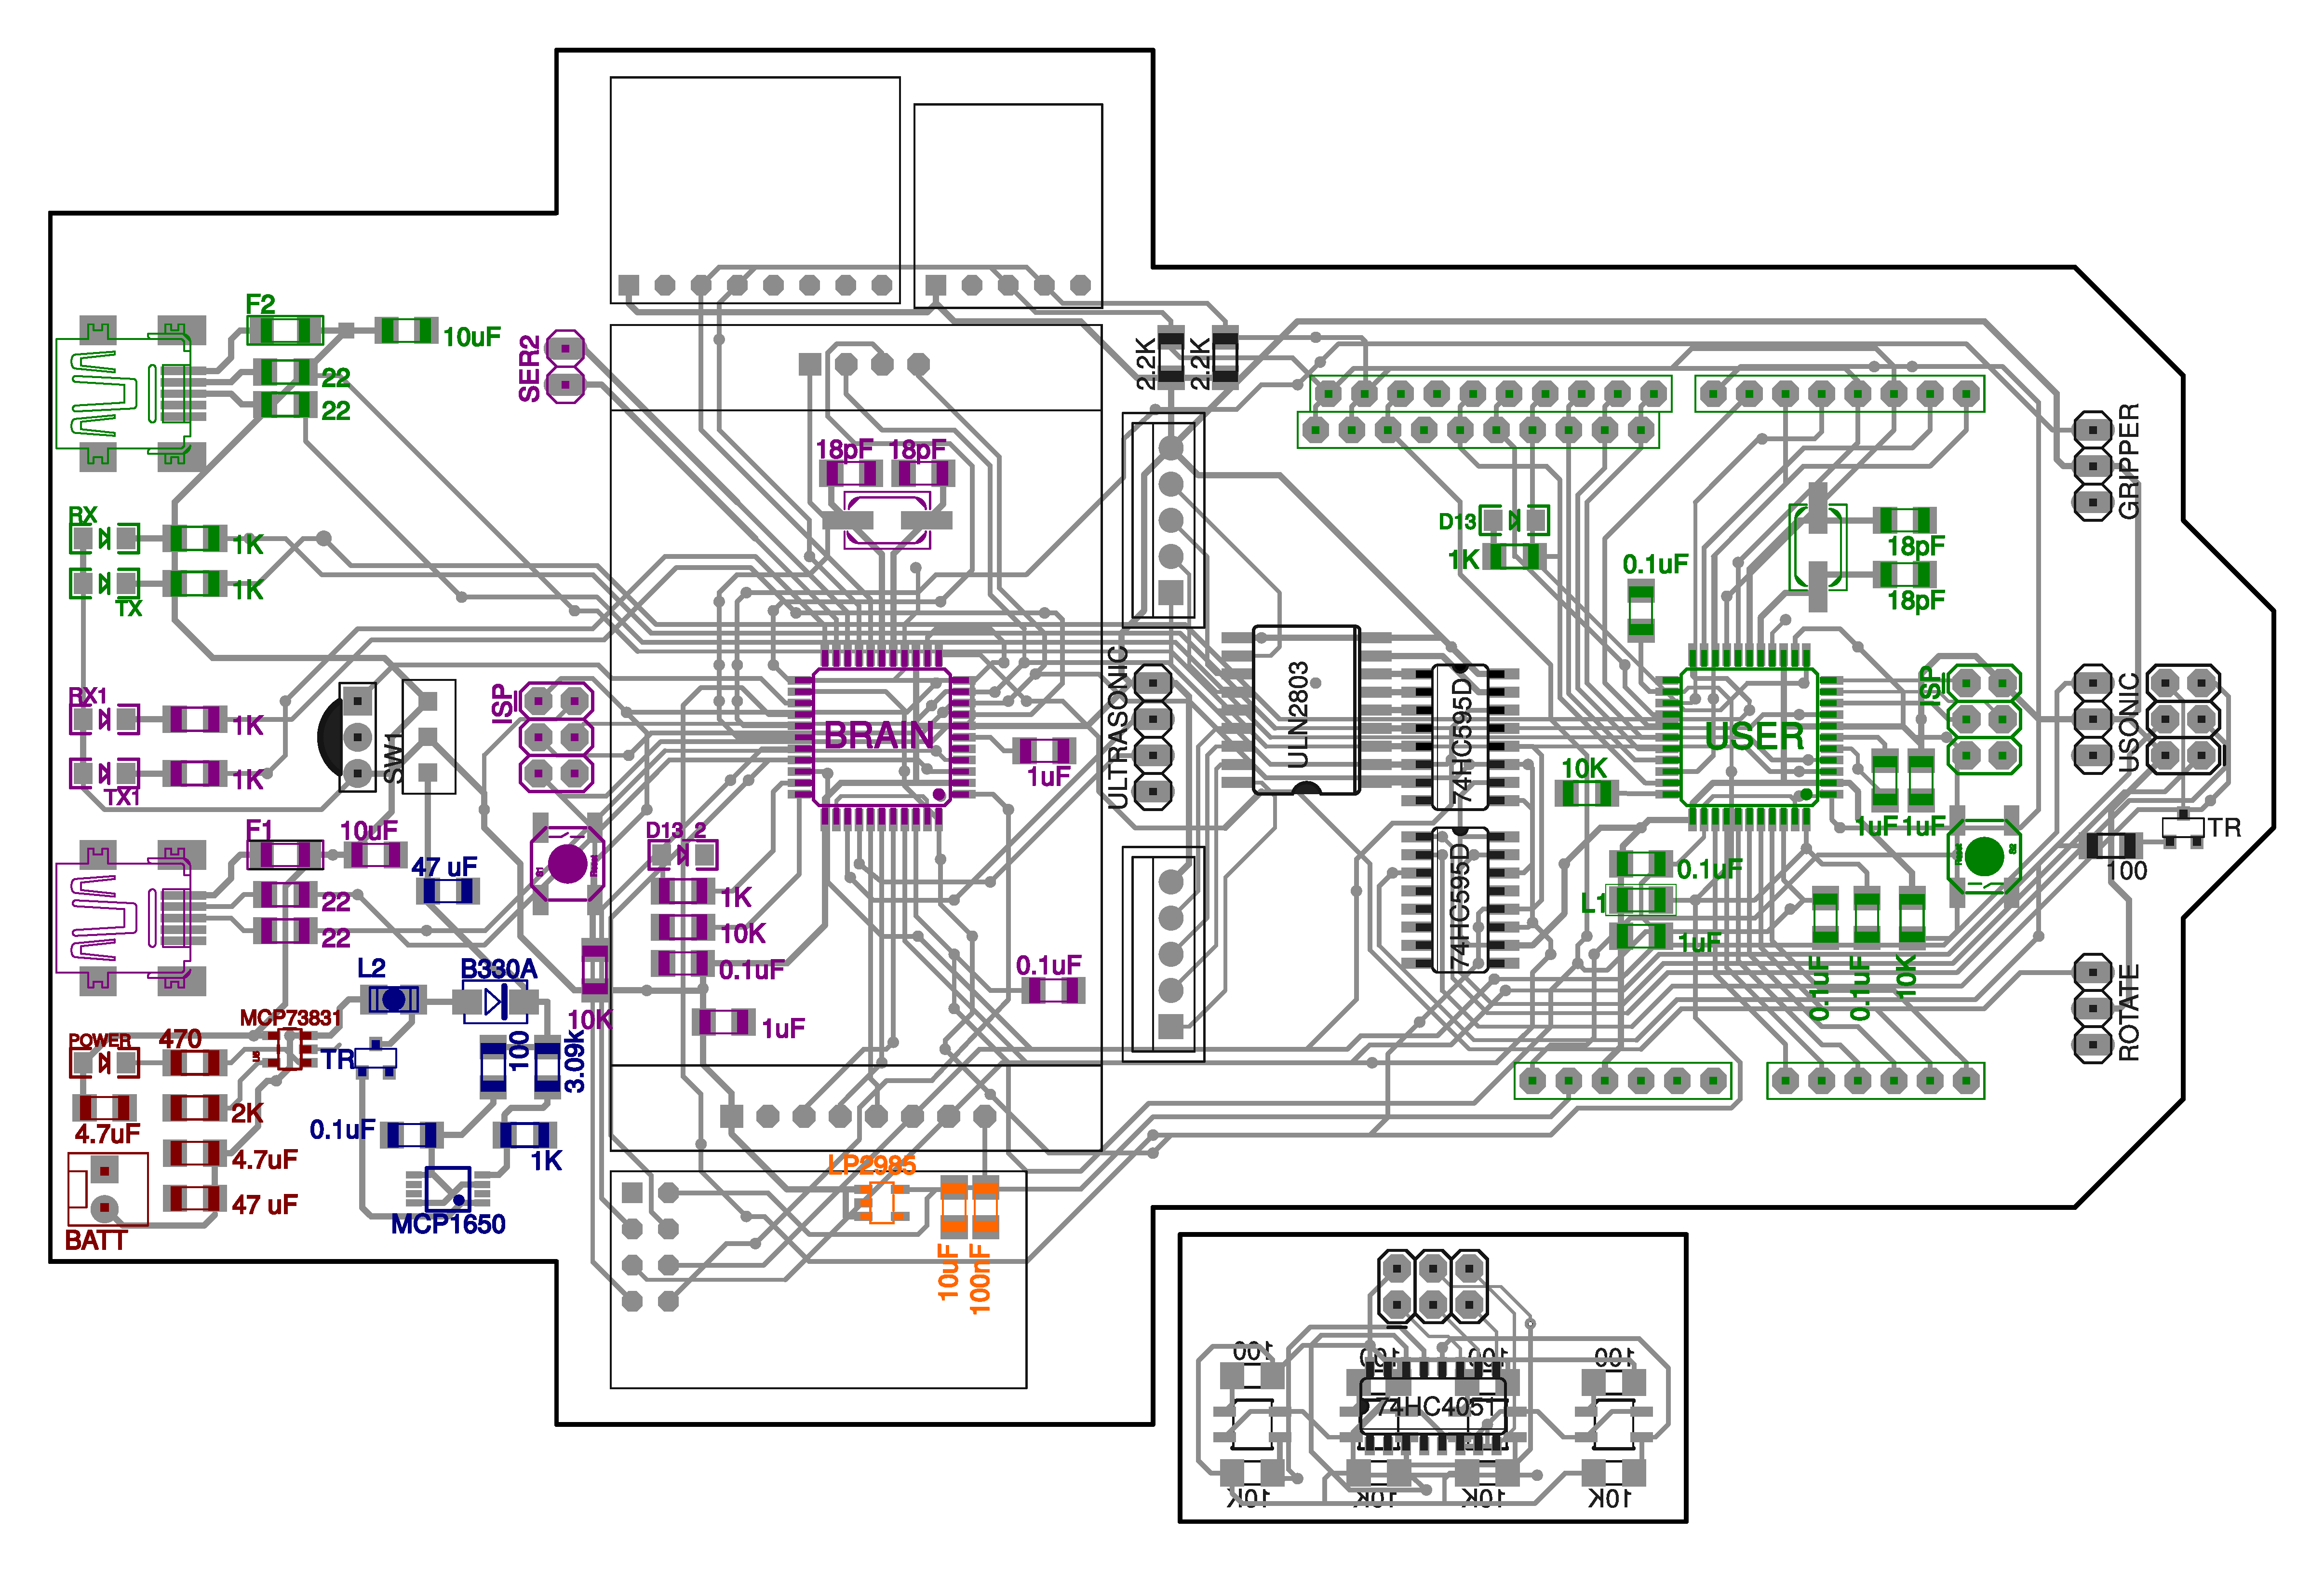
\includegraphics[width=\textwidth]{images/schematic/robot_schematic_brain.pdf}
  \caption{Robot schematic creation. Second Arduino Leonardo compatible circuit components are higlighted in purple.}
\end{figure}

In addition to the second Arduino Leonardo the motor control must be placed. In the design the ULN2803 violates the pcb layout recommendation since it is placed rotated by 180 degree. This was necessary to prevent unnecessary  trace routing efforts. The connectors for the motors are standard JST XH series connectors which match the connectors crimped to the stepper motors.

\begin{figure}[H]
  \centering
  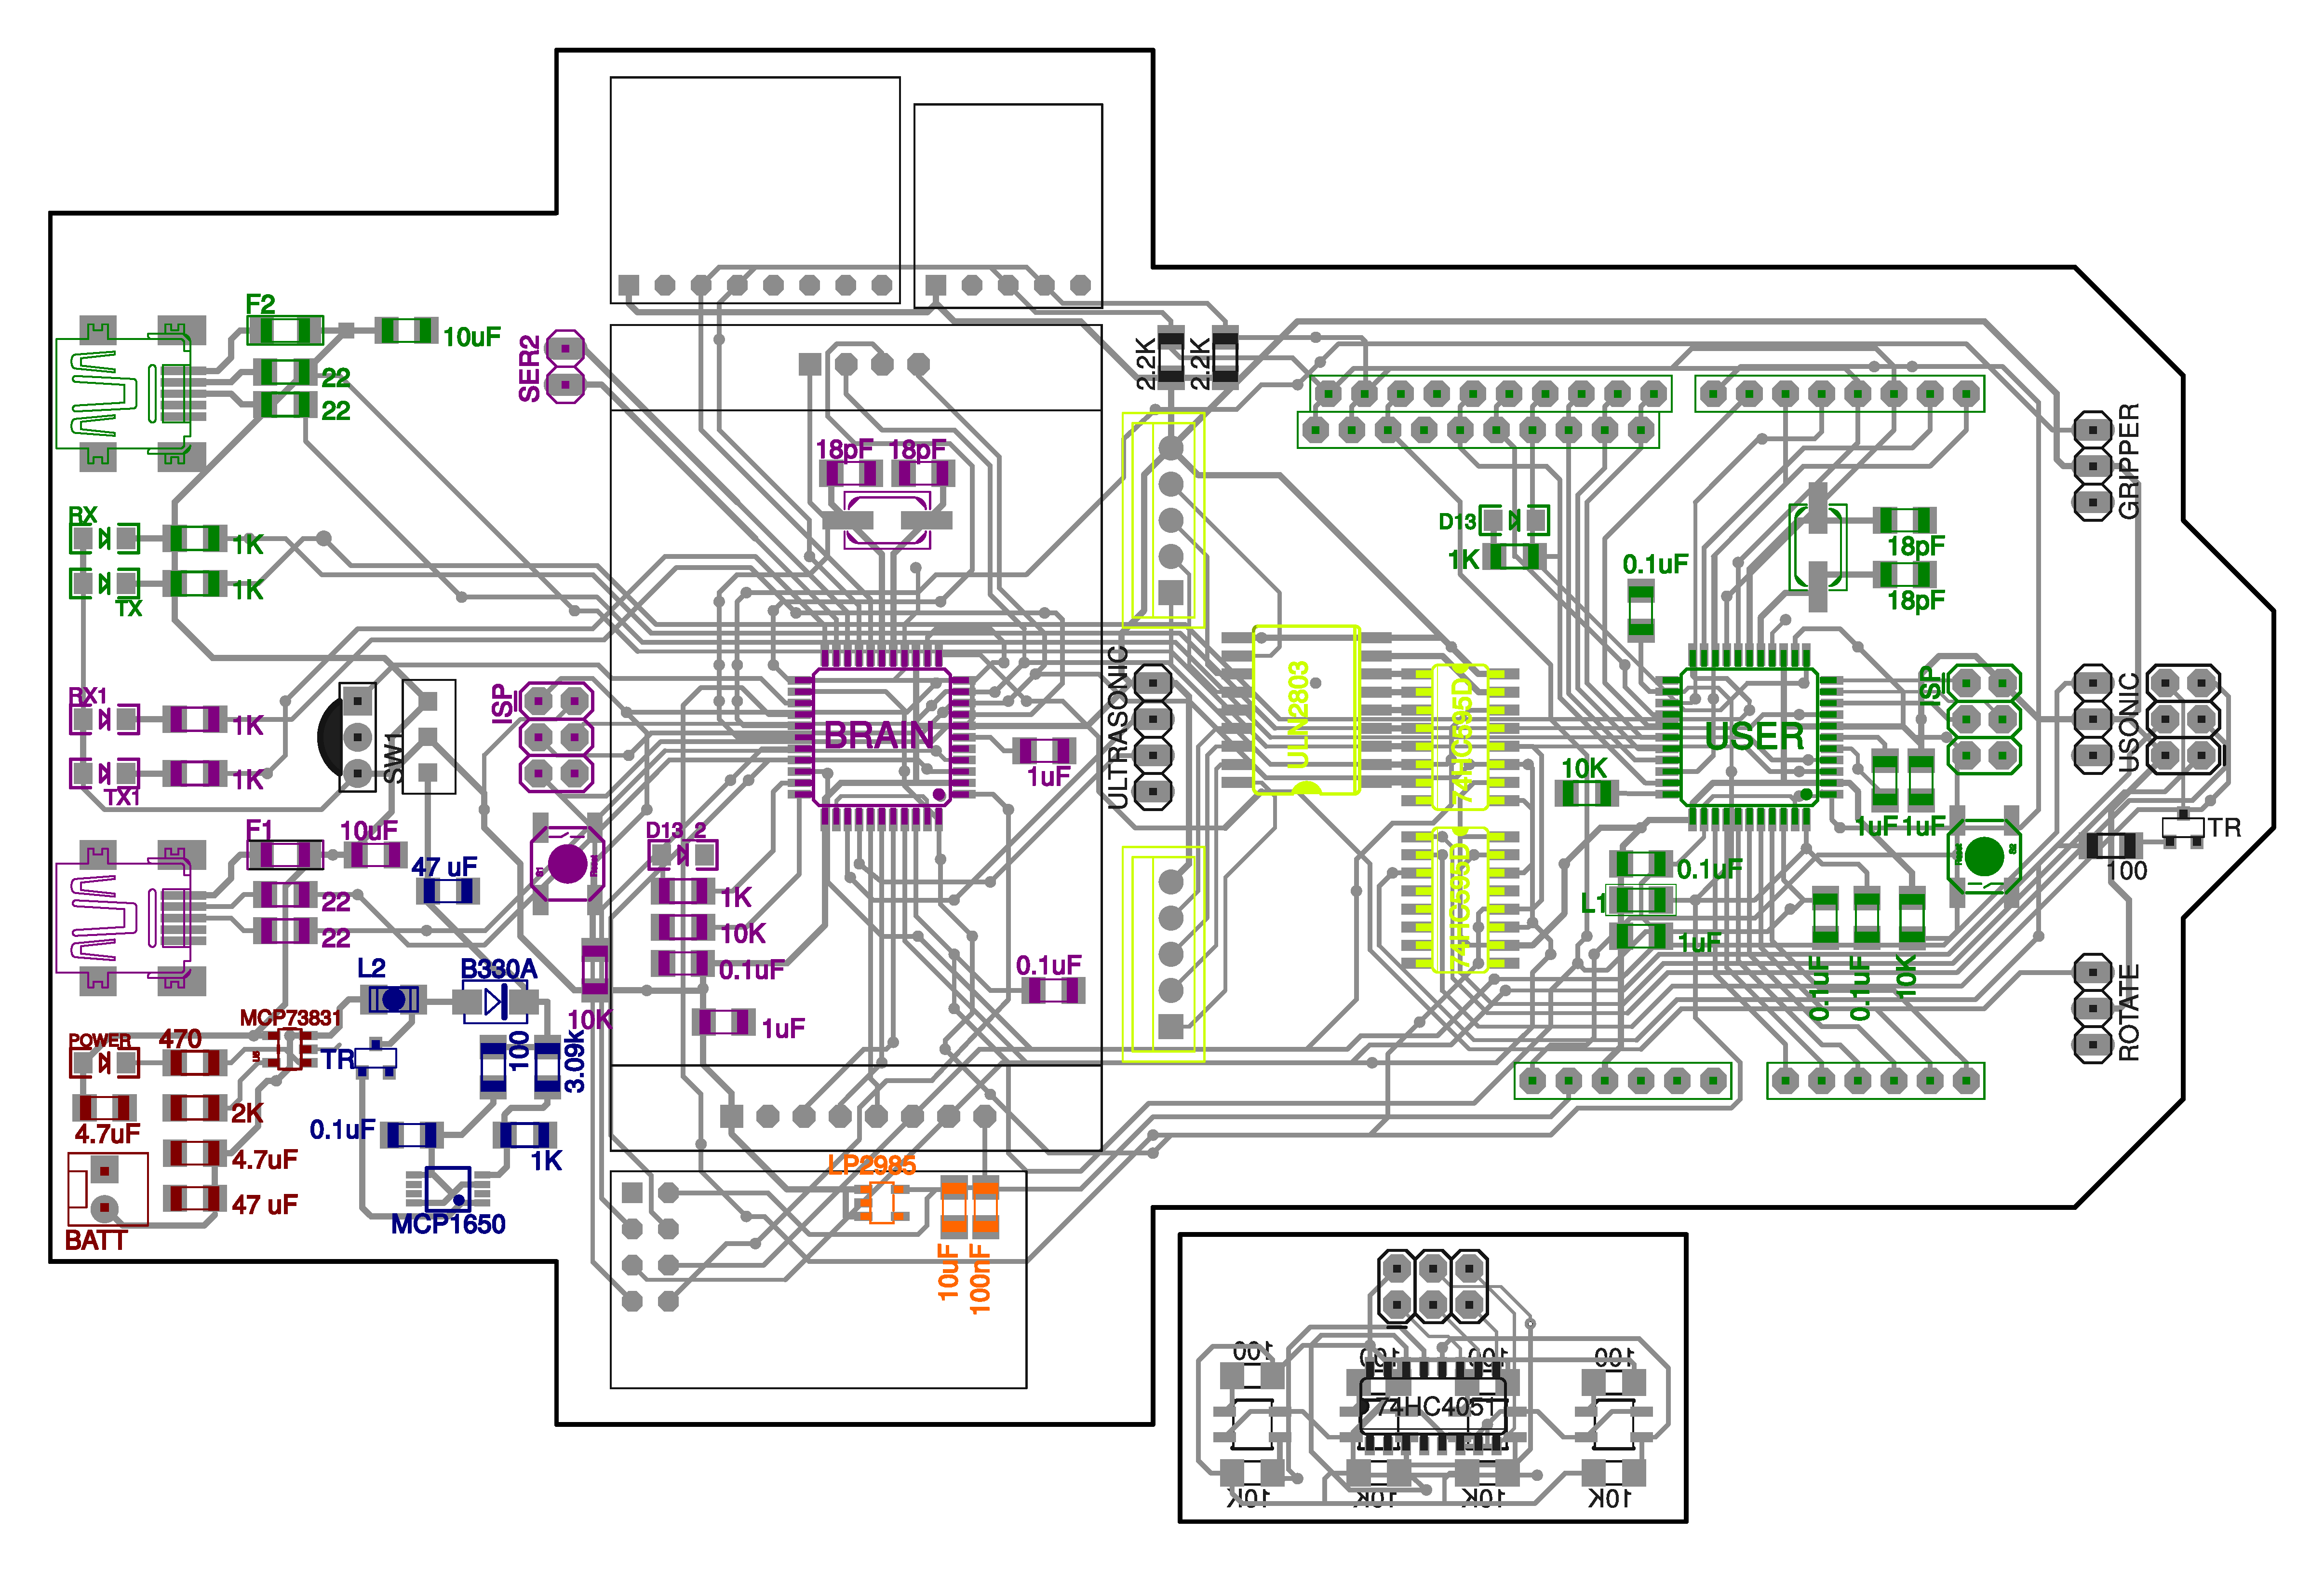
\includegraphics[width=\textwidth]{images/schematic/robot_schematic_motor.pdf}
  \caption{Robot schematic creation. Motor control circuit components are higlighted in lime.}
\end{figure}

To allow line sensing the robot features four infrared sensors with integrated LEDs and photodiodes. Placing them in a well defined spacing allows to scan an area for a line and therefore speeds up the process of finding the line to follow.

Since the sensors must be placed within a few millimetres above the ground, the components for the sensor are placed on a external board which has, similar to the main board, mounting holes for standard M3 screws. Externalizing the components also allows to externalize the rather large 74HC4051 multiplexer to save space on the main board. Connecting the sensor board to the main is achieved using a 6 pin flat ribbon cable connector.

% not needed.
%\begin{figure}[H]
%  \centering
%  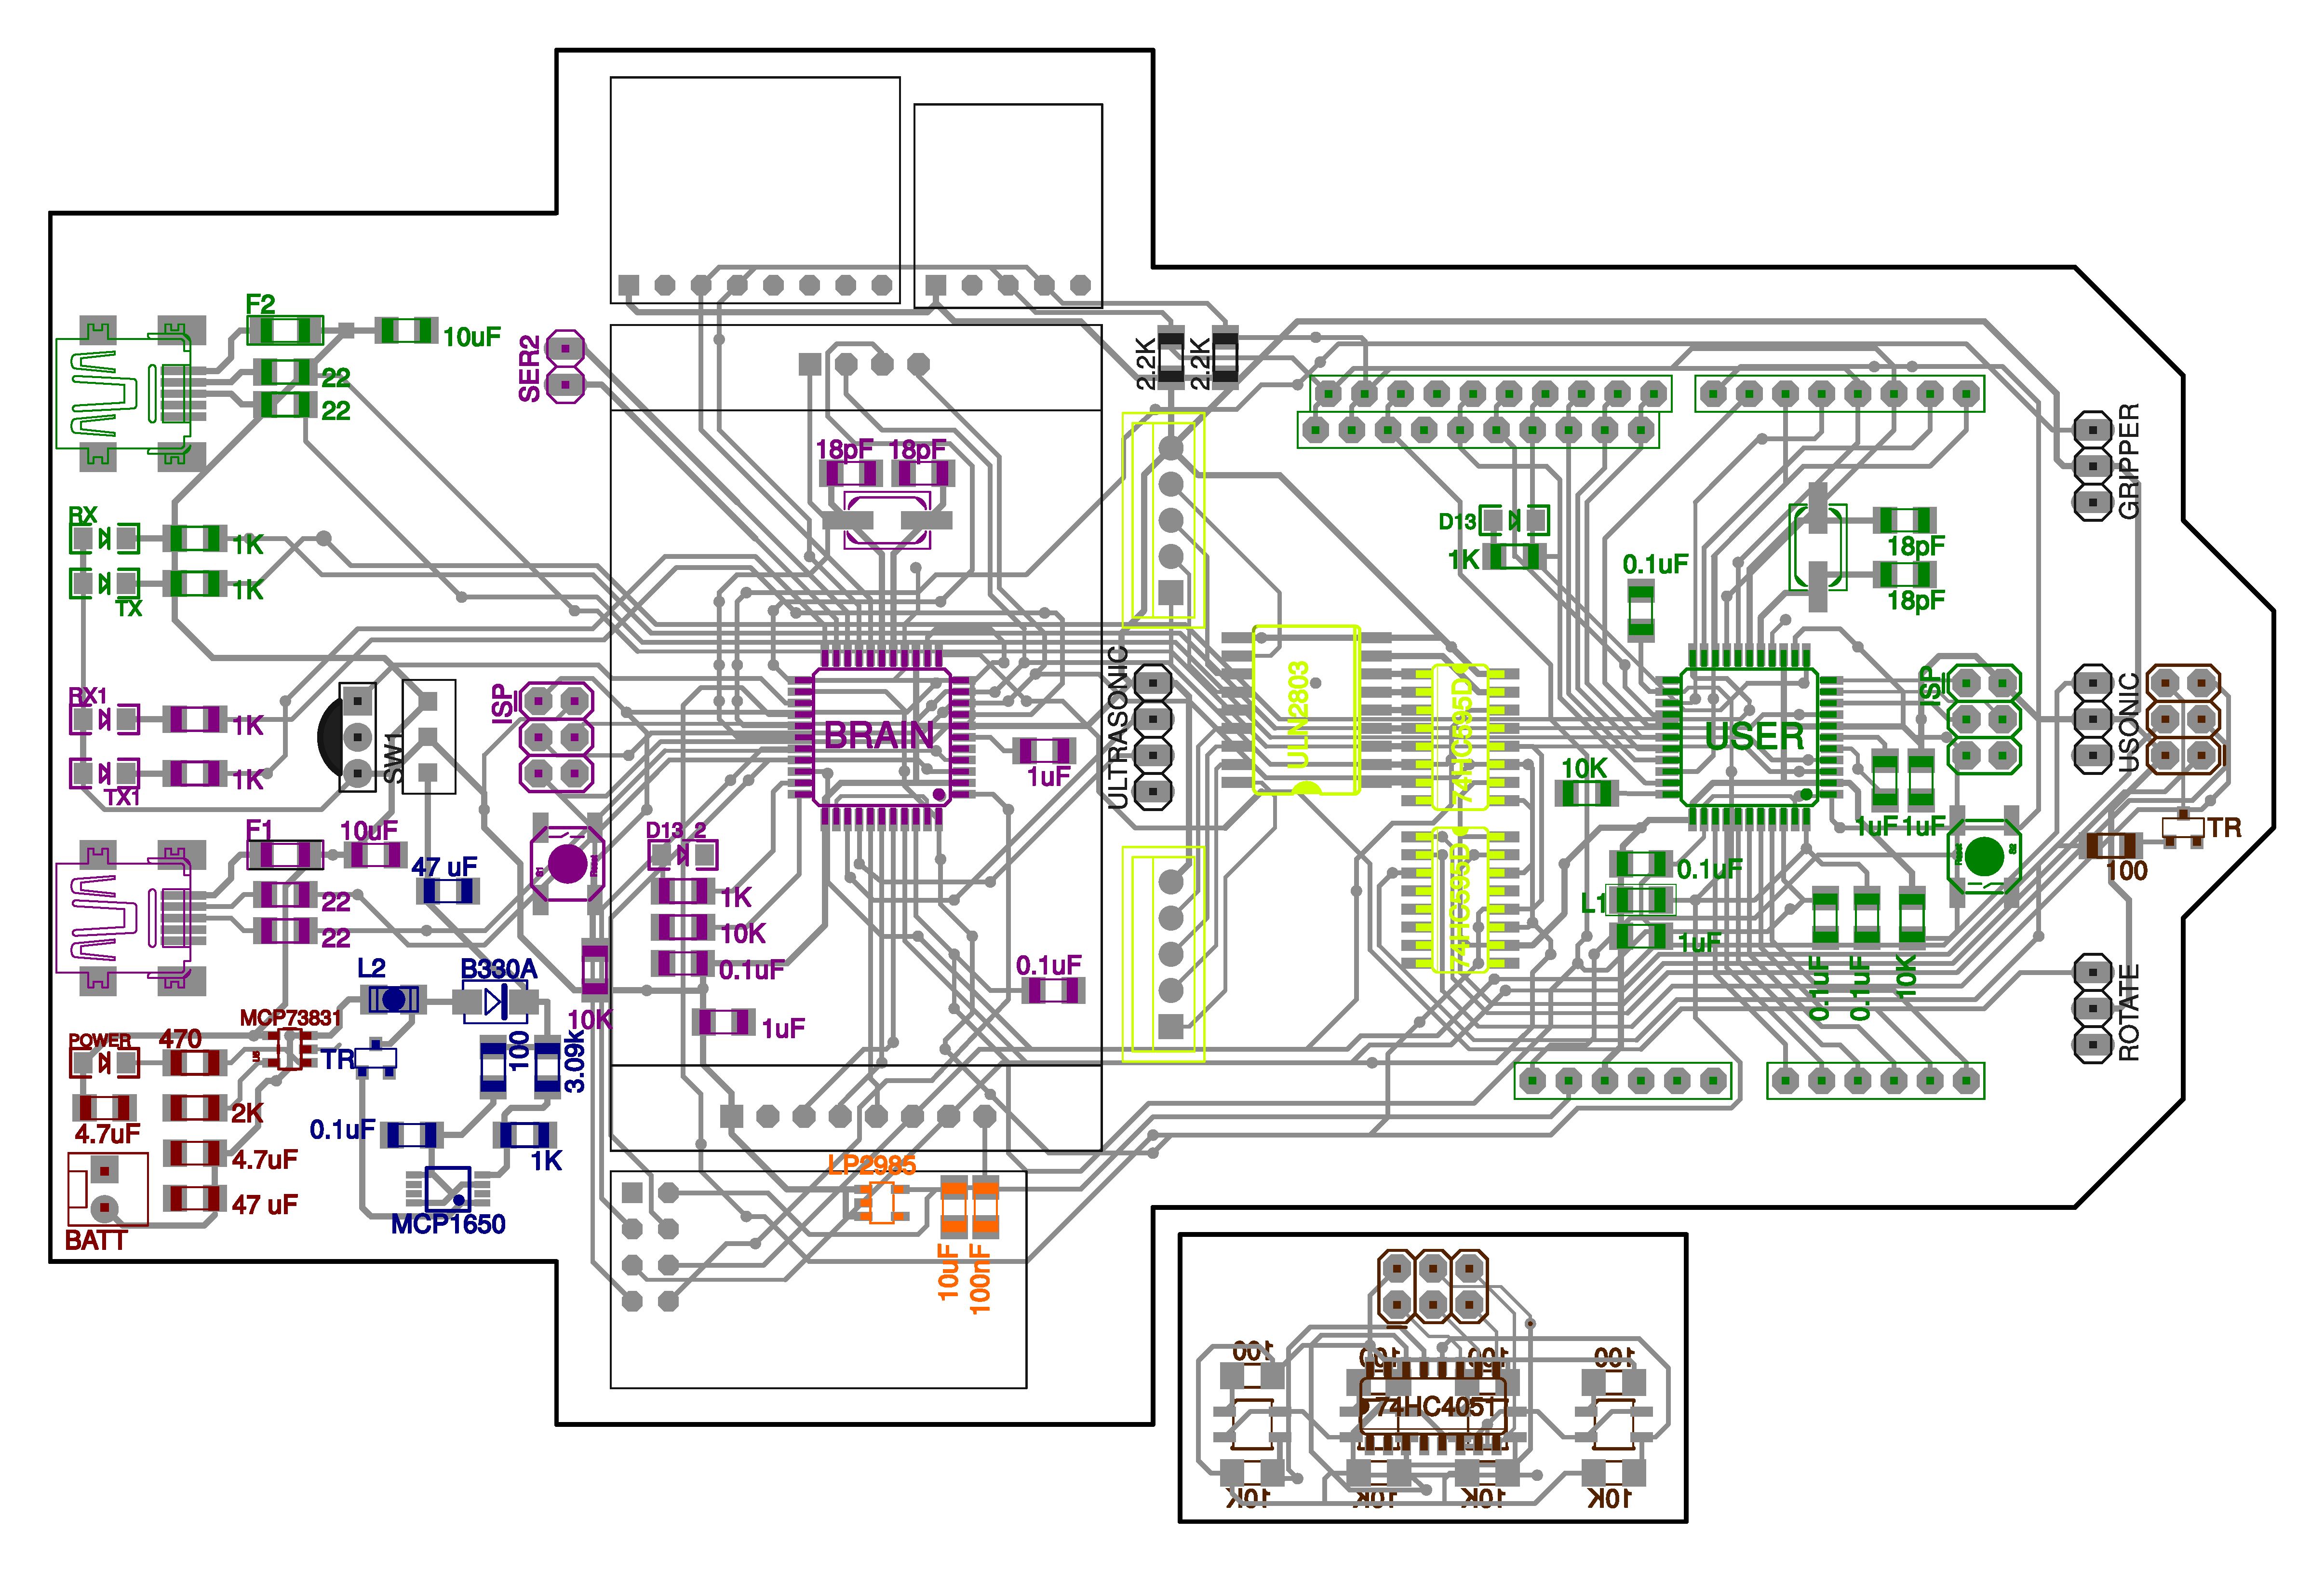
\includegraphics[width=\textwidth]{images/schematic/robot_schematic_sensor.pdf}
%  \caption{Robot schematic creation. Line sensing components are higlighted in brown.}
%\end{figure}
%
%
%\begin{figure}[H]
%  \centering
%  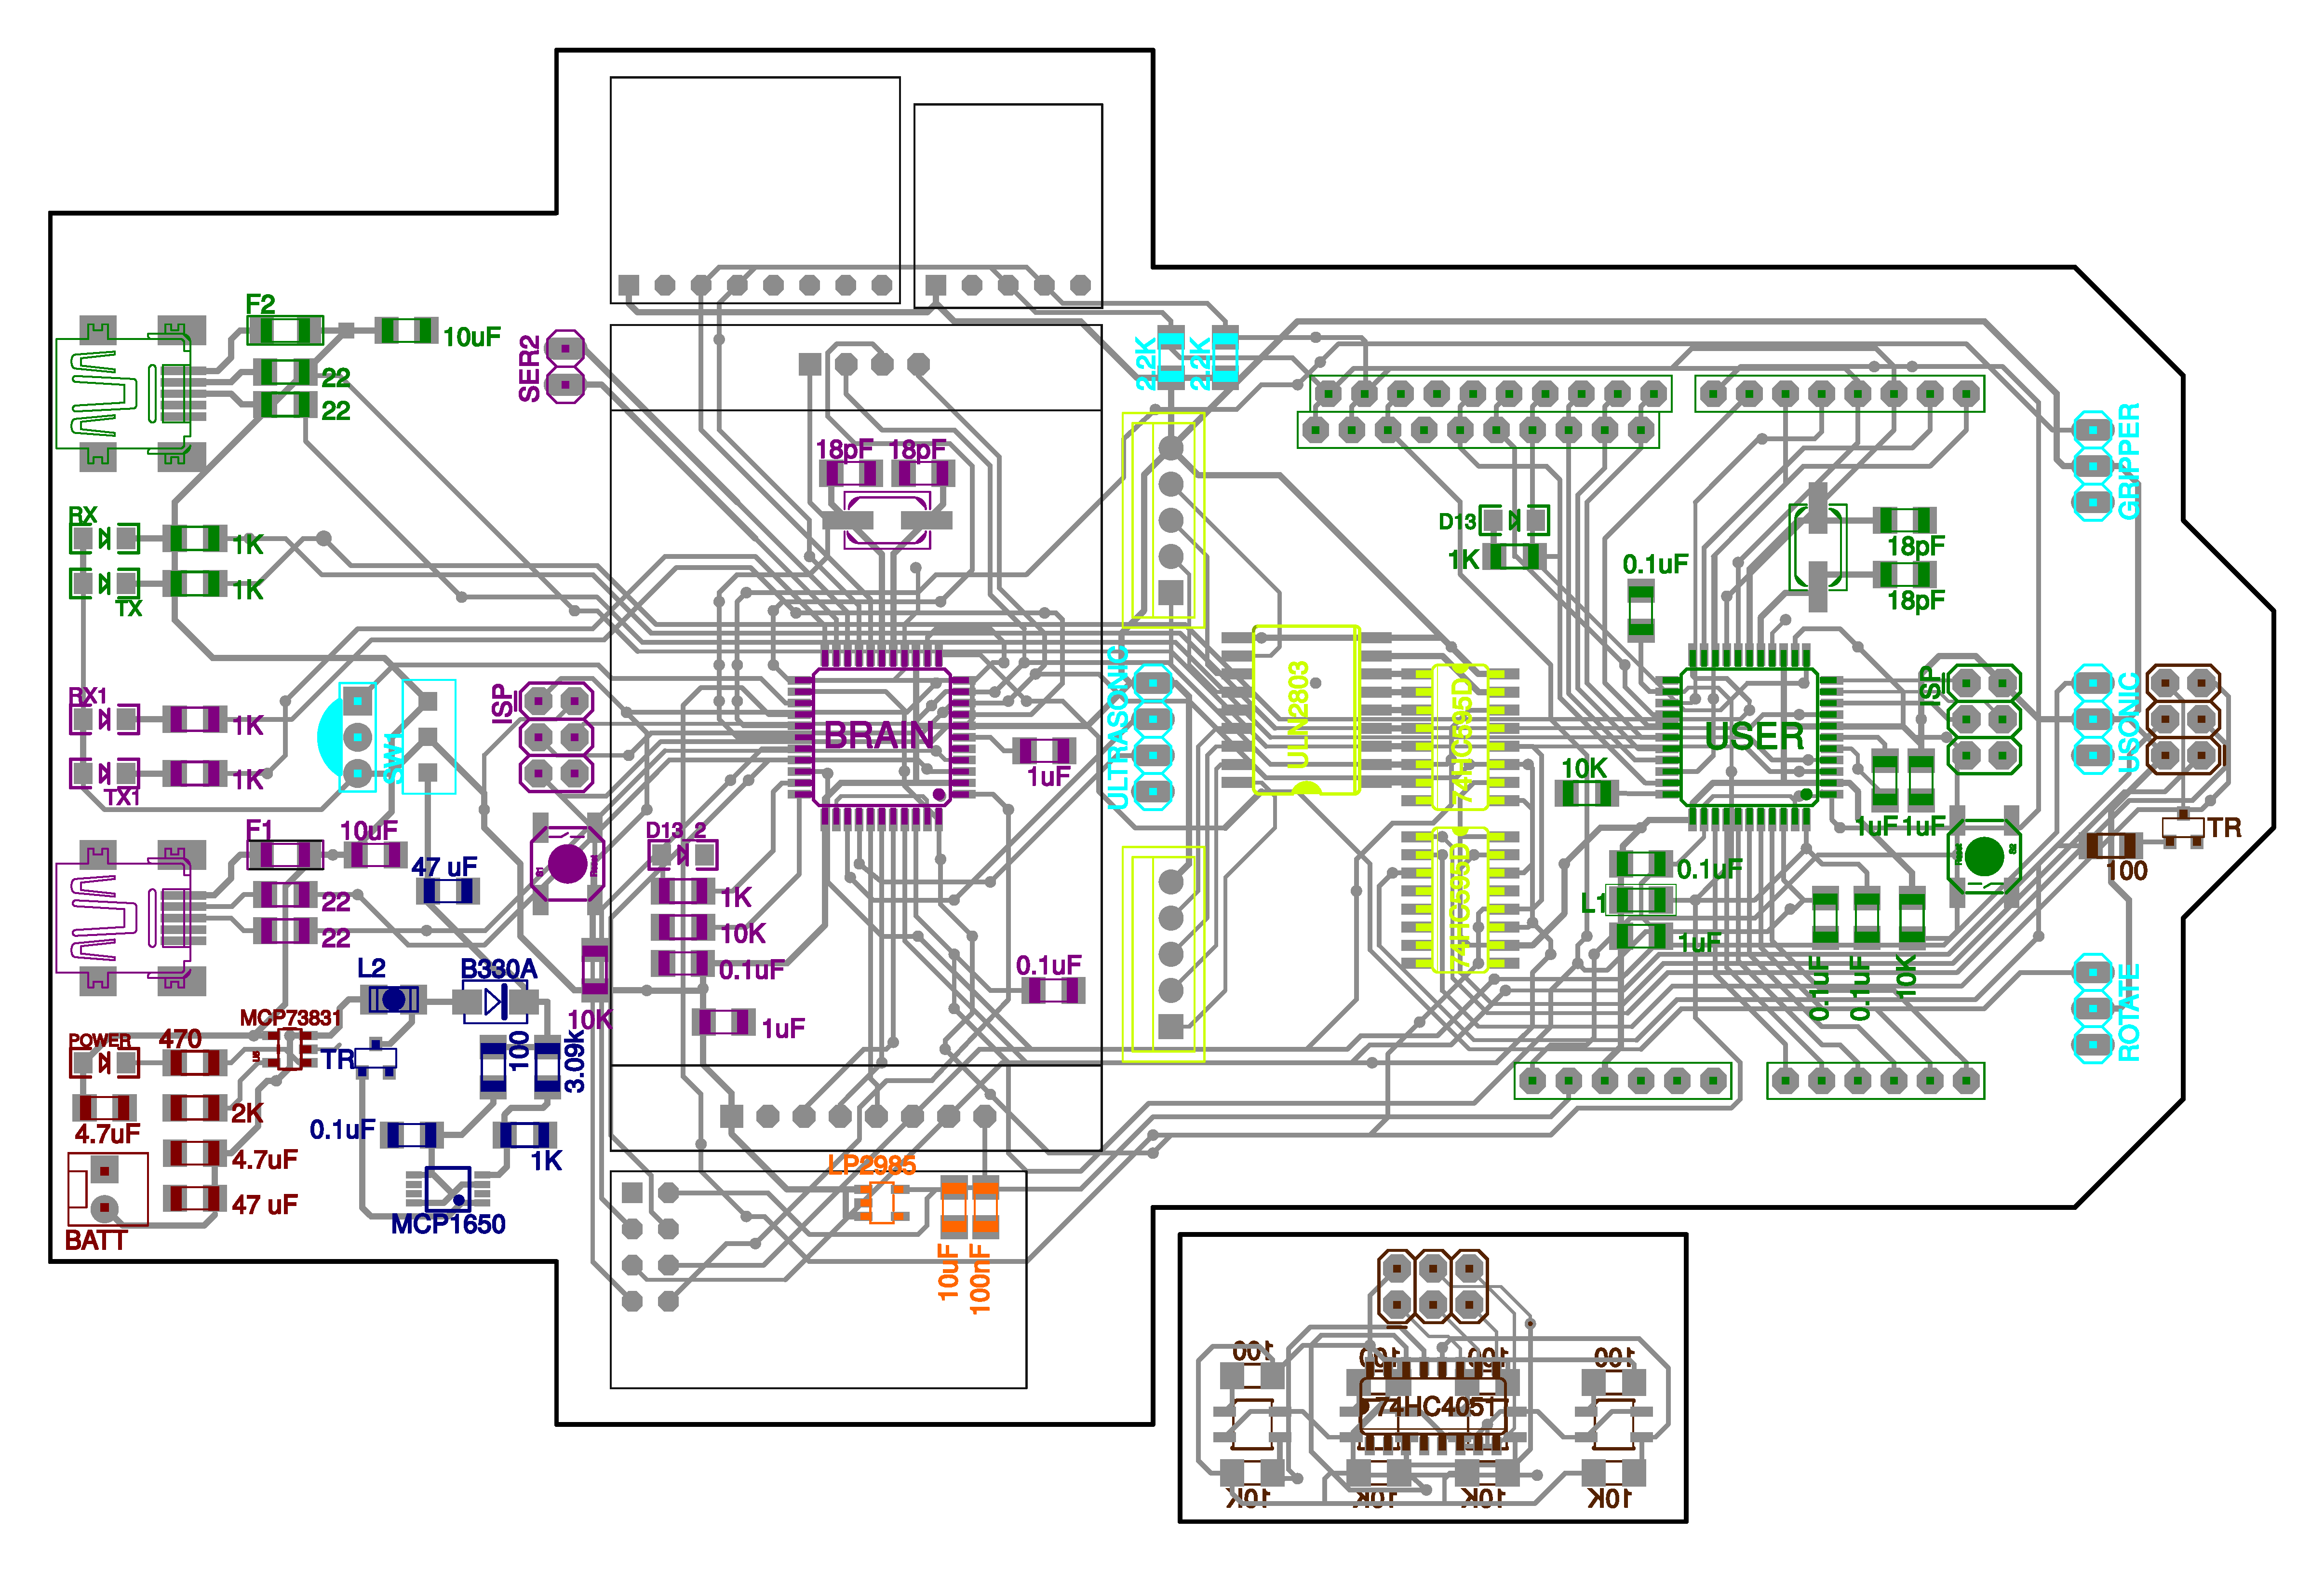
\includegraphics[width=\textwidth]{images/schematic/robot_schematic_addtional.pdf}
%  \caption{Robot schematic creation. Additional components are higlighted in aqua.}
%\end{figure}

Finally all other components are placed on the board as well. The power switch is positioned for easy reach and the IR reciever for maximum angle. Optional pull-up resistors for the I2C communication are placed near the I2C compass and I2C accelerometer + gyroscope module. 

Pins headers for the gripper servos and ultrasonic distance sensor rotation servos are placed in the front rear of the board since the servos will be located at the front of the robot. 

\begin{figure}[H]
  \centering
  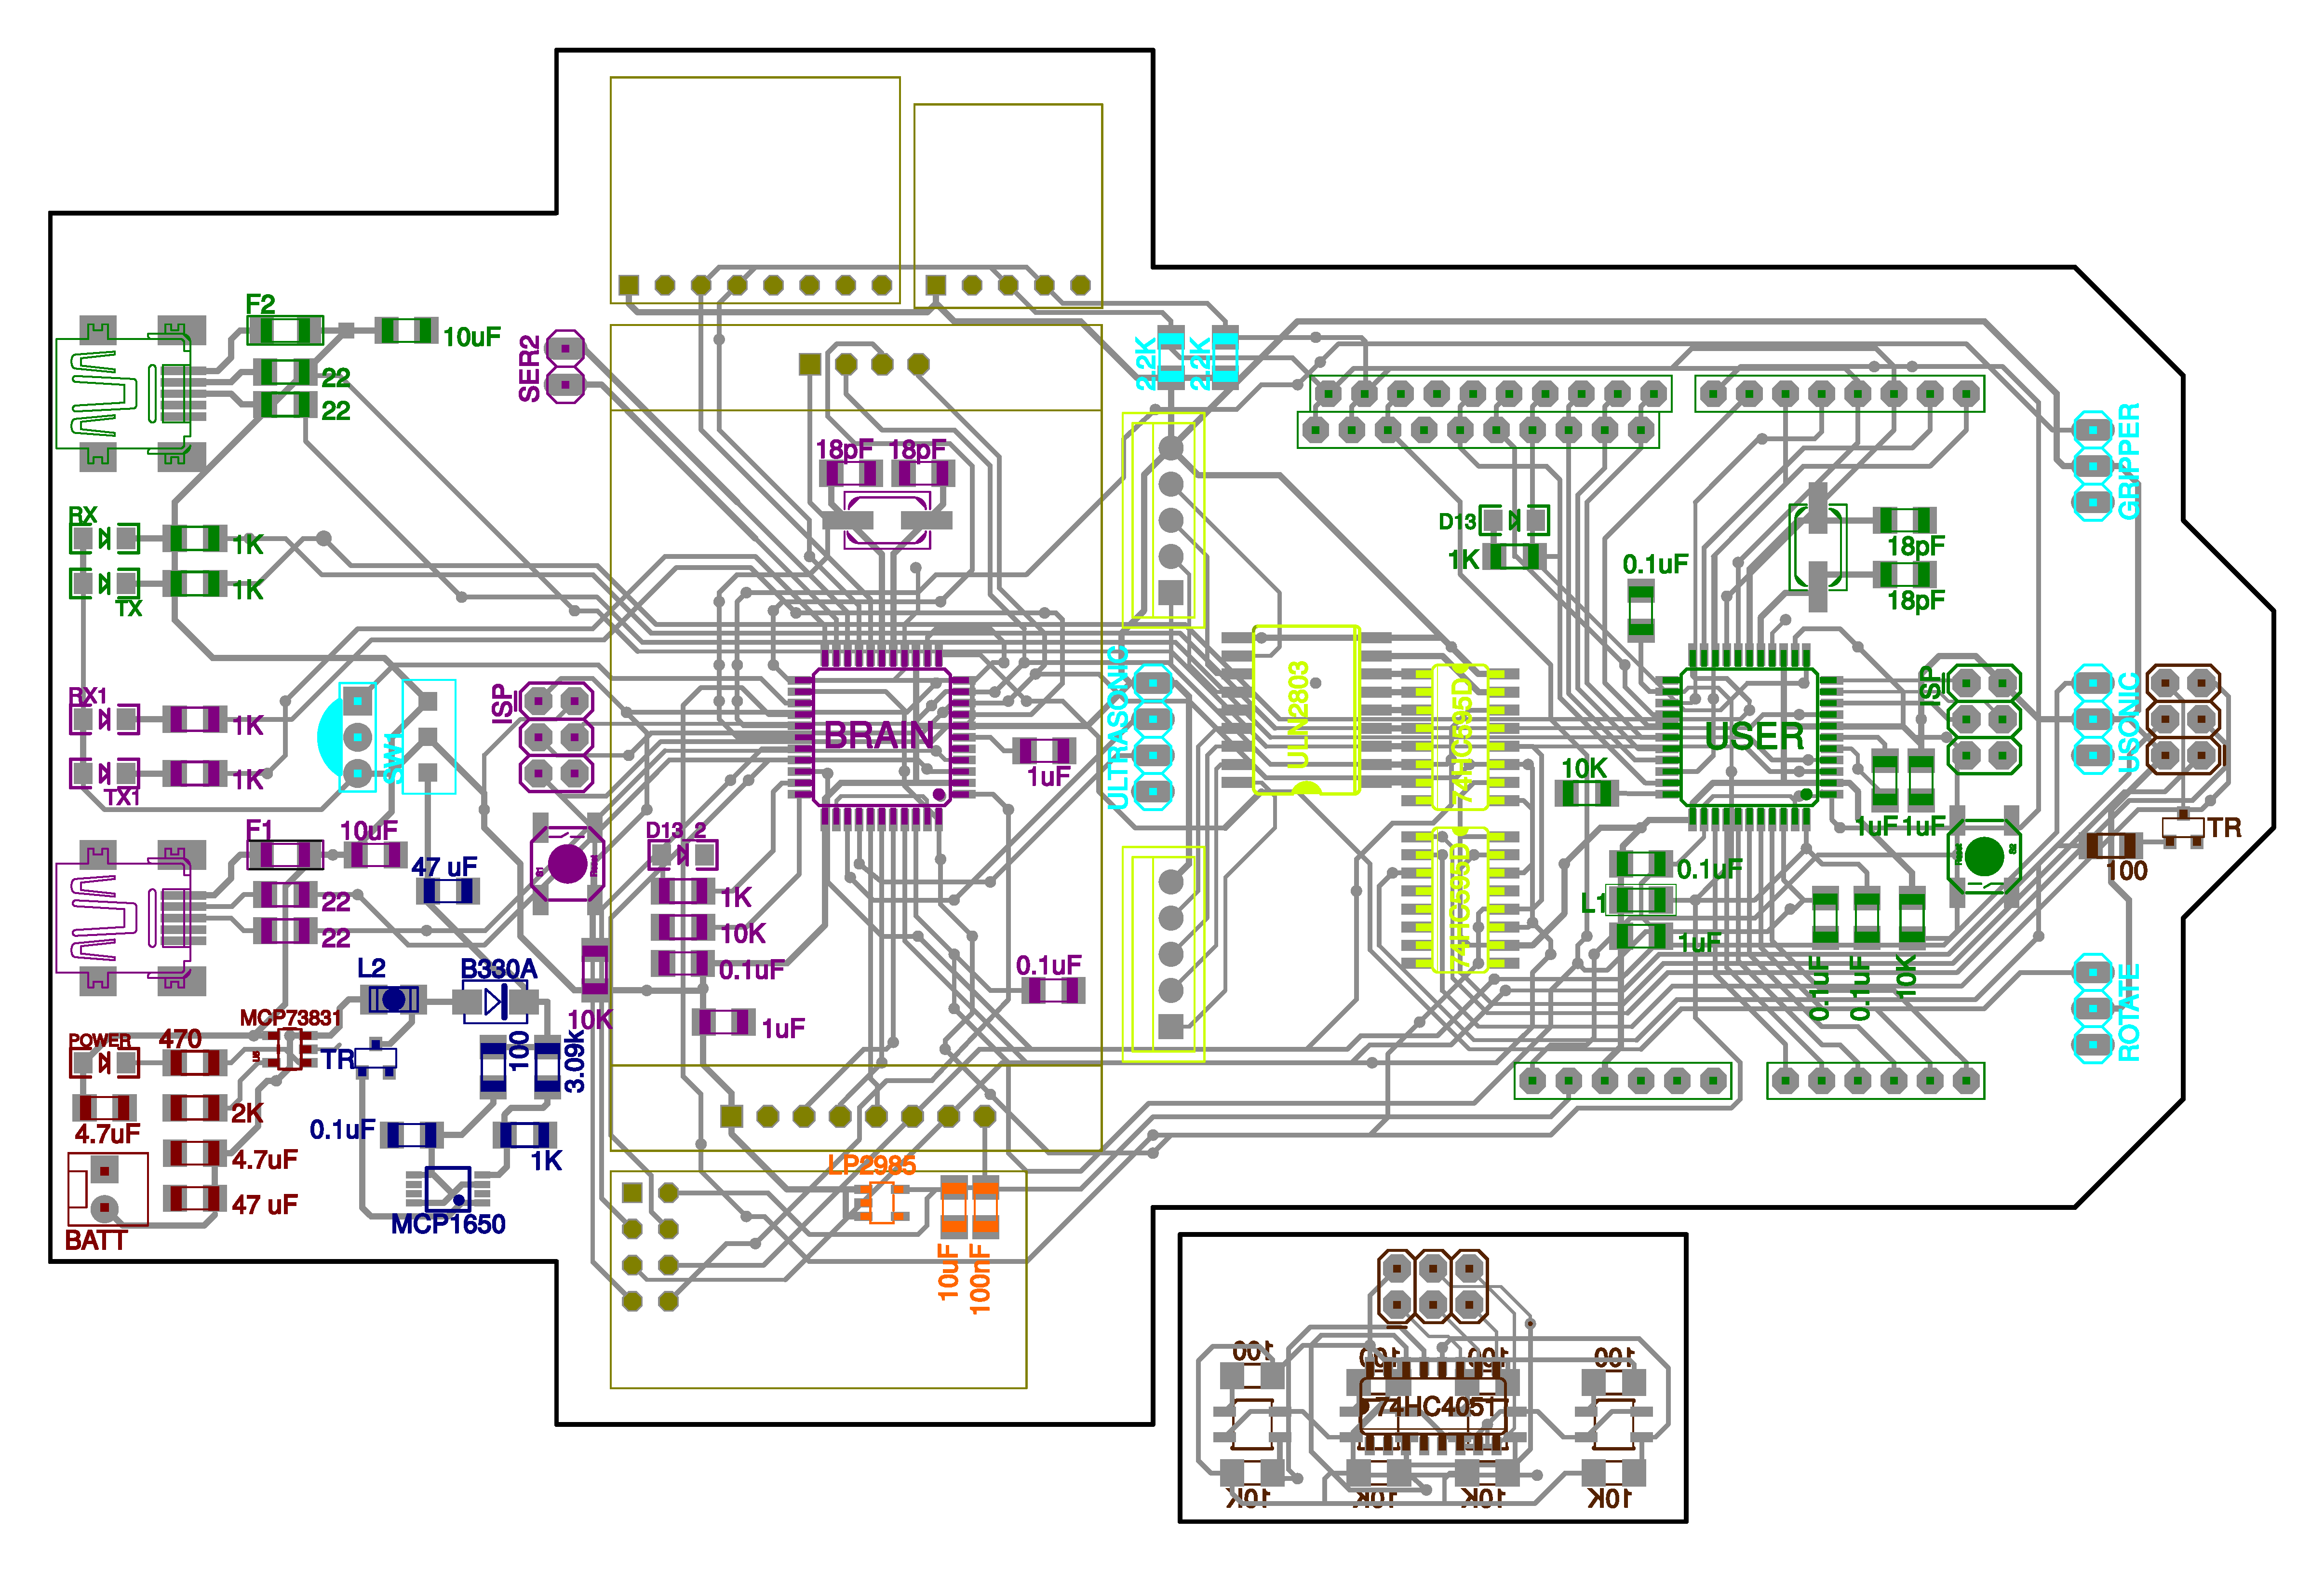
\includegraphics[width=\textwidth]{images/schematic/robot_schematic_optional.pdf}
  \caption{Robot schematic creation. Placeholder for optional components on breakout boards are higlighted in olive, additional components in aqua and line sensing components are highlighted in brown.}
\end{figure}



\section{Mechanical platform}
The robots PCB, motors, ball caster, gripper and sensors have to be assembled together. Therefore mechanical components are needed which hold the components to a common base. 

Possible materials for a base are plywood or acrylic glass. Both materials can be shaped using a laser cutting machine.  Plywood is relatively cheap (3mm thick plywood costs about 6\euro per square meter) but smells like burned wood after laser cutting. Acrylic glass is more expensive than plywood (about 30\euro per square meter for colorless variants, about 40\euro for coloured acrylic glass) but does not smell after laser cutting. In terms of stability acrylic glass is more stable than plywood since it does not bend as much as plywood does.

For making holders for the stepper motors and a stand for the ultrasonic sensor, 90 degree angled connections must be made. Instead of glueing the pieces together a new popular method with M4 screws and nuts is used. One part gets cutouts and a hole for the screw, the other parts gets a t-slot which fits the cutout and a screw with a nut. The robot features two types of t-slots: a small type and a wider type for mechanically stressful connections.

When the part fitting the cutout is fitted into it, a basic 90 degree connection is made. To stabilize it a nut is placed in the t-slot and the two parts are fastened together with a screw. An illustration by MAKE magazine shows the principle well:
 
\begin{figure}[H]
  \centering
  \begin{subfigure}{0.48\textwidth}
  \centering
  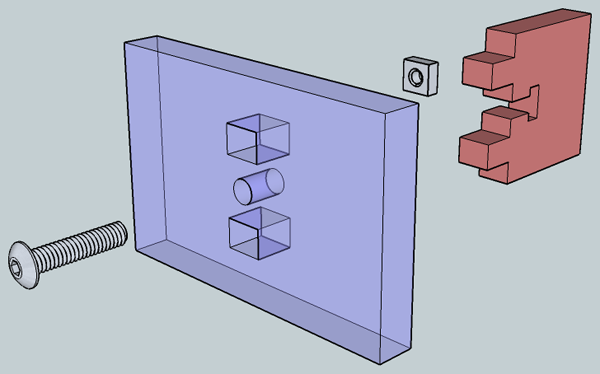
\includegraphics[width=0.9\linewidth]{images/captive-square-nut-joint-exploded.png}
  \caption{exploded view}
  \end{subfigure}
  \begin{subfigure}{0.48\textwidth}
  \centering
  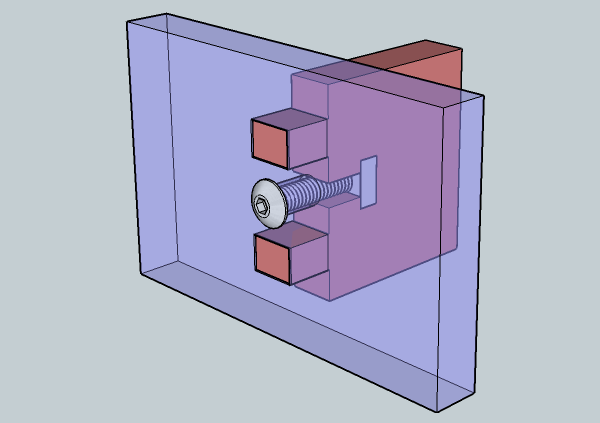
\includegraphics[width=0.9\linewidth]{images/captive-square-nut-joint-imploded.png}
  \caption{imploded view}
  \end{subfigure}
  \caption{Captive nut joint illustration by MAKE magazine (from \url{http://makezine.com/2011/10/06/clever-captive-square-nut-cnc-panel-joint/})}
\end{figure} 
 
Different to the illustration by MAKE magazine the junctions designed for the robot are narrowing for easier fit. The main platform where the PCB is located features the mentioned junctions for stepper motors and the ultrasonic distance sensor.

\begin{figure}[H]
  \centering
  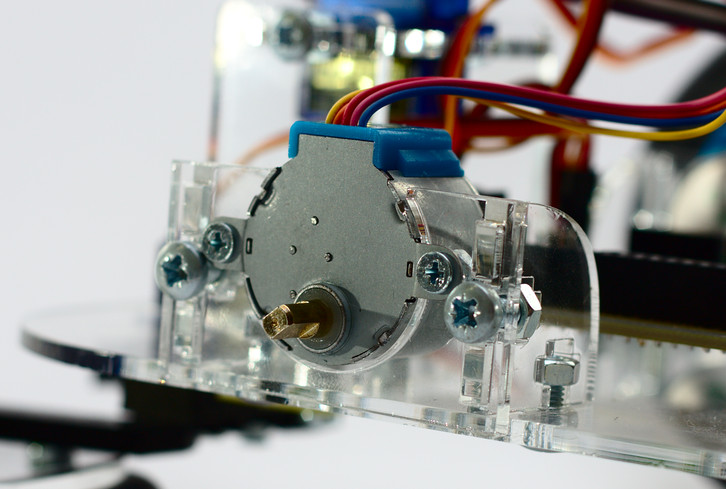
\includegraphics[width=0.8\textwidth]{images/30_motormount1.jpg}
  \caption{Motor mount using t-slots (CC-BY-SA Ben Oswald)}
\end{figure}

Advantages of the t-slots over glue or elbow connectors are the low costs (less than one cent for screw and nut), the mechanically stable connection and the adjustment possibilities when the connection accidentally loosens. 
 
\subsection{Wheels}

The 28BJY-48 stepper motor shaft enables to attach a wheel. Since plastic wheels are expensive, a new wheel was developed which fits the motor. The most difficult part is the connection between the motor shaft and the wheel.

There are three possible connections which can be made between the motor and the wheel:
\begin{description}
\item[Glue] Glue is a possible solution but lacks reproducible results, is difficult to apply in the right amount and may harm during the build (e.g. when using superglue).
\item[Press-fit] Building a press-fit connection e.g. by 3D printing a mount gives a strong connection but may wears out after a while. Since 3D printing is not very accurate, making a press-fit connection is difficult.
\item[Press-fit plus screws] Combining a press-fit connection with screws anchored in the 3D printed mount pressing against the motor shaft results in a strong connection. If needed the screws can be adjusted to provide more pressure.
\end{description}

Having a press-fit connector with screws still lacks a wheel attached to it. Since the components should be cheap and off the shelf, acrylic glass is one potential material.

\begin{figure}[H]
  \centering
  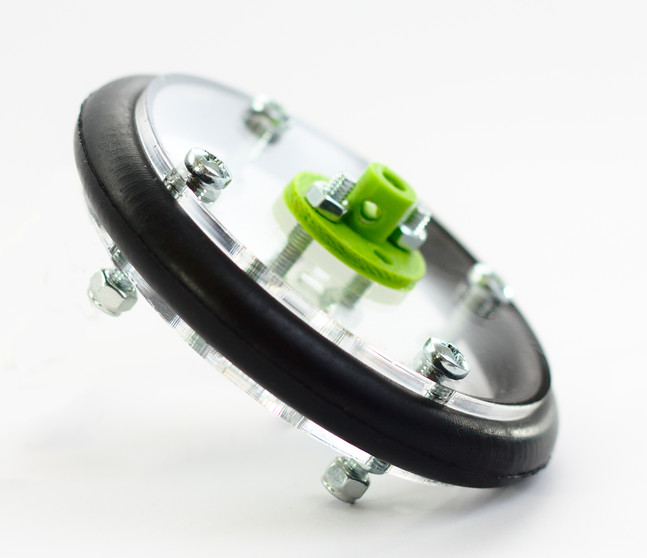
\includegraphics[width=0.8\textwidth]{images/30_wheel_full.jpg}
  \caption{3D printed wheel connector with wheel (CC-BY-SA Ben Oswald)}
\end{figure}

Acrylic only is not well suited for a wheel since it does not provide enough grip to the ground. A solution is to use two acrylic glass plates with an O-ring pressed between them using M4 screws with nuts. The rubber of the O-ring provides lots of grip and is relatively cheap (1.5\euro at the local DIY-market).

\chapter{Conclusion}
To conclude the success in robot construction, the robot must be evaluated using the assessment criteria already introduced in the chapter "State of the Art". 

\begin{figure}[H]
  \centering
  \begin{subfigure}{0.48\textwidth}
  \centering
  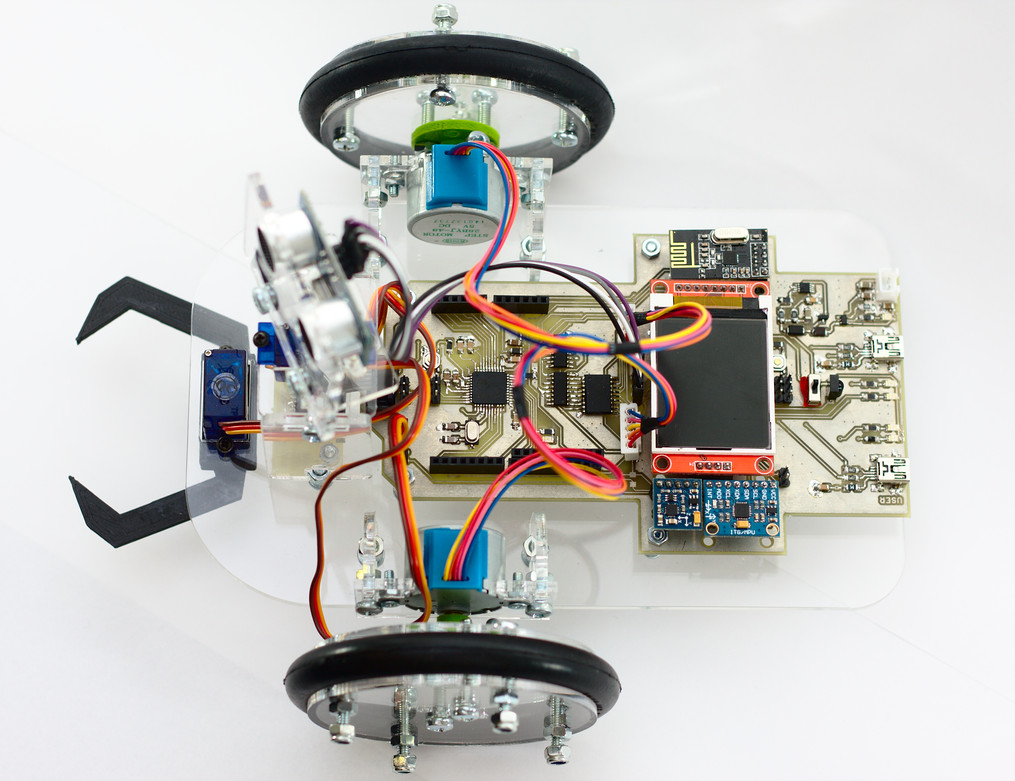
\includegraphics[width=0.9\linewidth]{images/30_robot_top.jpg}
  \caption{Top view of the robot}
  \end{subfigure}
  \begin{subfigure}{0.48\textwidth}
  \centering
  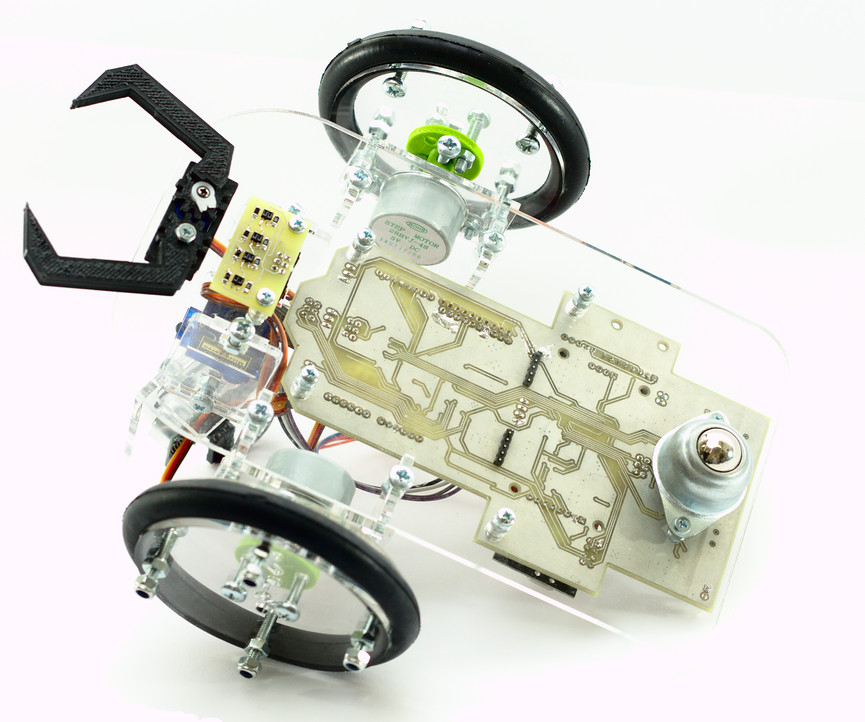
\includegraphics[width=0.9\linewidth]{images/30_robot_bottom.jpg}
  \caption{Bottom view of the robot}
  \end{subfigure}
  \caption{Views of the robot (CC-BY-SA Ben Oswald)}
\end{figure} 

\begin{longtabu} to \textwidth { X[1,l] X[1,l] X[4,l]}
\toprule
Assessment Criteria    & Rating & Description \\
\midrule
Affordable      & \stars{5}    & With a price tag of 31.28\euro for the base kit and 41.51\euro for the kit with all extensions\footnote{without VAT, based on mass production calculation for hundred units.} the robots costs are below the maximum price of 100\euro.\\
Educational     & \stars{4}     & Assembling the robot and its components includes a unique learning experience and allows the explanation of each part. The Arduino compatibility enables the usage of comprehensive tutorials and how-to documentation. Learning material for teachers is not yet supplied. \\
Sustainable       & \stars{5}     &  The robot integrates charging circuit for the Lithium-polymer batteries which eliminates the need of a dedicated battery charger and therefore reduces the amount of electrical waste. All components can be easily replaced by beginners by either changing the pre-soldered modules or solder a new component. No tantalum capacitors are included.\\
Extendable & \stars{5}      &  Sensors and a display can be directly plugged in to extend the functionality of the robot. Unused ports are broken out onto pin headers. Fully compatible Arduino headers allow the usage of Arduino shields.\\
Trouble-free & \stars{4} & Building the robot is made easy doe to super sized SMD components. When possible 1206 sized parts are used. Some ICs on the board are hard to solder (e.g. the MCP 1650) and should come pre-assembled to avoid frustration.\\
Open-Source & \stars{5} & The design file for laser cutting, the pcb schematic and board files are available under a Creative Commons Attribution Share-Alike license.\\
\bottomrule
\caption{Robot evaluation}
\label{tbl:arduinorobot_eval}
\end{longtabu}

All in all the robot reaches a rating of 4.6 of a maximum of 5. The main advantages are the low price, the extensibility and the Arduino compatibility. Disadvantages are located in the assembly since some parts are difficult to assemble.

\begin{figure}[H]
  \centering
  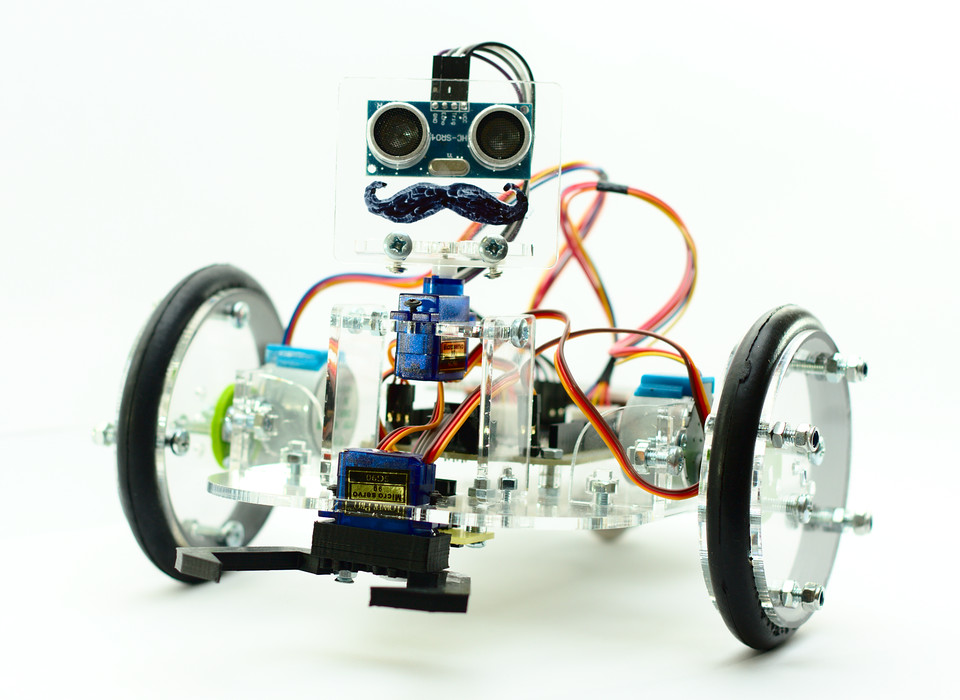
\includegraphics[width=0.8\textwidth]{images/30_robotfront.jpg}
  \caption{Roboter front view (CC-BY-SA Ben Oswald)}
\end{figure}


Anyway, the robot designed has the potential to be used for educational purposes. The modular design leads to low initial costs which should be affordable for everyone. Since the robot ought to generate revenue for the producing company, other sources for income must be available. The robot addresses this issues by enabling the sale of optional modules with a higher profit margin so that income and revenue can be generated.

